\documentclass[semifinal]{cpecmu}

%% options for survey
\cpetrue

%% This is a sample document demonstrating how to use the CPECMU
%% project template. If you are having trouble, see "cpecmu.pdf" for
%% documentation.

\projectNo{S006-2/66}
\acadyear{2023}

\titleTH{ระบบสนับสนุนการตัดสินใจซื้อขายสินทรัพย์ด้วยฟัซซีโลจิก}
\titleEN{Fuzzy Logic in Market Trading Decision Support System}

\author{ธนัตถ์ ตั้งอั้น}{Tanat Tangun}{630610737}
\author{ธนวัตน์ บำเพ็งพันธุ์}{Thanawat Bumpengpun}{630610736}

\cpeadvisor{sansanee}
\cpecommittee{kasemsit}
\committee{รศ.ดร.\,นิพนธ์ ธีรอำพน}{Assoc.\,Prof.\,Nipon Theera-Umpon, Ph.D.}

%% Some possible packages to include:
\usepackage[final]{graphicx} % for including graphics
\usepackage{booktabs, siunitx}
\usepackage{placeins}

%% Add bookmarks and hyperlinks in the document.
\PassOptionsToPackage{hyphens}{url}
\usepackage[colorlinks=true,allcolors=Blue4,citecolor=red,linktoc=all]{hyperref}
\def\UrlLeft#1\UrlRight{$#1$}

%% Needed just by this example, but maybe not by most reports
\usepackage{afterpage} % for outputting
\usepackage{pdflscape} % for landscape figures and tables. 

%% Some other useful packages. Look these up to find out how to use
%% them.

% \usepackage{csquotes}
% \usepackage[
%   backend=biber,
%   sorting=none,
%   style=numeric,
% ]{biblatex}
% \addbibresource{sampleReport.bib}
% \DeclareLanguageMapping{thai}{english}

% \usepackage{natbib}    % for author-year citation styles
% \usepackage{txfonts}
% \usepackage{appendix}  % for appendices on a per-chapter basis
% \usepackage{xtab}      % for tables that go over multiple pages
% \usepackage{subfigure} % for subfigures within a figure
% \usepackage{pstricks,pdftricks} % for access to special PostScript and PDF commands
% \usepackage{nomencl}   % if you have a list of abbreviations

%% if you're having problems with overfull boxes, you may need to increase
%% the tolerance to 9999
\tolerance=9999

\bibliographystyle{unsrt}
% bibliographystyle{IEEEbib}

% \% renewcommand{\topfraction}{0.85}
% \% renewcommand{\textfraction}{0.1}
% \% renewcommand{\floatpagefraction}{0.75}

%% Example for glossary entry
%% Need to use glossary option
%% See glossaries package for complete documentation.
\ifglossary
  \newglossaryentry{lorem ipsum}{
    name=lorem ipsum,
    description={derived from Latin dolorem ipsum, translated as ``pain itself''}
  }
\fi

%% Uncomment this command to preview only specified LaTeX file(s)
%% imported with \include command below.
%% Any other file imported via \include but not specified here will not
%% be previewed.
%% Useful if your report is large, as you might not want to build
%% the entire file when editing a certain part of your report.
% \includeonly{chapters/intro,chapters/background}

\setotherlanguage{english}
\begin{document}
\maketitle
\makesignature

\ifproject
\begin{abstractTH}
ระบบเพื่อช่วยนักลงทุนในการเทรดโดยนำอินดิเคเตอร์ทางเทคนิคและปัจจัยอื่นๆ ของผู้ใช้งานที่ใช้ในการวิเคราะห์การซื้อ และการขายมาสร้างอินดิเคเตอร์ตัวใหม่ที่ช่วยตัดสินใจโดยใช้ Fuzzy logic 
ซึ่งต่างจากอินดิเคเตอร์ทางเทคนิคแบบดั้งเดิม เนื่องจากสามารถเอามุมมองการวิเคราะห์ส่วนตัวของผู้ใช้งานใส่เข้าไปในอินดิเคเตอร์ตัวนี้ได้ โดยอินดิเคเตอร์ตัวนี้จะรับข้อมูลอย่างเช่น RSI, 
MA, การทำกำไรของสินทรัพย์, ความผันผวนของตลาด และข้อมูลอื่นๆ ที่ผู้ใช้งานอาจจะต้องการ ในขณะที่เอาต์พุตคือสัญญาณการซื้อ และการขาย หรือสัญญาณวิเคราะห์อื่นๆ 
ที่ผู้ใช้งานต้องการสร้างขึ้น ด้วยวิธีดังกล่าวอินดิเคเตอร์ของเราจะสามารถช่วยนักลงทุนในการจัดการกับข้อมูลหลายๆปัจจัยที่ผู้ใช้งานใช้ในการวิเคราะห์ ออกมาเป็นสัญญาณใหม่เพียง 1 หรือ 2 
สัญญาณ เพื่อใช้ในการช่วยตัดสินใจ เราจะสร้างเว็บแอพพลิเคชั่นจากไอเดียดังกล่าวข้างต้น แล้วเผยแพร่เพื่อเก็บผลตอบรับจากผู้ใช้งาน
\end{abstractTH}

\begin{abstract}
In this work, we propose a system to help process technical indicators and other factors to make a new indicator based on 
fuzzy logic, which unlike traditional technical indicators it incorporates subjective view of investor into it too. 
Our indicitor will recieve input such as RSI, MA, profitiblity of an assets, volatility in the market and others that user may 
need, while the outputs are the buy and sell signals or other signal that user may want to create. This way our indicator can help 
user represent a bigger amount of information to a 1 or 2 signals and use this to help in decision-making. 
We will create a web application based on this idea, publish it and gather feedback from user.
\end{abstract}

\iffalse
\begin{dedication}
This document is dedicated to all Chiang Mai University students.

Dedication page is optional.
\end{dedication}
\fi % \iffalse

\begin{acknowledgments}
Your acknowledgments go here. Make sure it sits inside the
\texttt{acknowledgment} environment.

\acksign{2020}{5}{25}
\end{acknowledgments}%
\fi % \ifproject

\contentspage

\ifproject
\figurelistpage

\tablelistpage
\fi % \ifproject

% \abbrlist % this page is optional

% \symlist % this page is optional

% \preface % this section is optional


\pagestyle{empty}\cleardoublepage
\normalspacing \setcounter{page}{1} \pagenumbering{arabic} \pagestyle{cpecmu}

\chapter{\ifenglish Introduction\else บทนำ\fi}

\section{\ifenglish Project rationale\else ที่มาของโครงงาน\fi}
ในปัจจุบัน, นักลงทุนมีการใช้การวิเคราะห์ทางเทคนิค (Technical Analysis) เพื่อช่วยให้การซื้อขายสินทรัพย์ในระยะสั้นได้กำไรสูงสุดเท่าที่เป็นไปได้
ซึ่งก็มักจะมีการใช้ตัวชี้วัดทางเทคนิค (Technical Indicators) หลายๆ อัน ในการที่จะพยายามหาจุดเข้าซื้อ หรือจุดขาย โดย 
ตัวชี้วัดทางเทคนิคเหล่านี้ส่วนใหญ่แล้วเป็นการคำนวณทางสถิติที่ใช้ ราคาย้อนหลัง, ปริมาณการซื้อขายย้อนหลัง, หรืออื่นๆ ในการ
คำนวณค่ามาเพื่อที่จะพยายามทำนายทิศทางของตลาด ซึ่งเราสามารถตีความหมายค่าของตัวชี้วัดทางเทคนิคด้วยเกณฐ์บางอย่าง เช่น 
สำหรับ RSI (Relative Strength Index) วิธีตีความหมายโดยทั่วไปคือ ถ้า RSI มากกว่า 70 หมายความว่าตลาดอยู่ใน
ภาวะซื้อมากเกินไปให้ขาย และถ้า RSI น้อยกว่า 30 หมายความว่าตลาดอยู่ในภาวะขายมากเกินไปให้เข้าซื้อ

ผู้จัดทำคิดว่าสามารถทำได้ดีกว่าการตีความหมายแบบในตัวอย่างก่อนหน้านี้ โดยใช้ Fuzzy Rule ในการตีความหมายจะให้ผลลัพธ์ที่ดีกว่าเนื่องจากตลาด
ซื้อขายสินทรัพย์น้้นมีความผันผวนและไม่แน่นอน ซึ่ง Fuzzy Logic นั้นสามารถทำงานได้ดีในการตีความ และใช้ข้อมูลที่คลุมเครือและไม่แน่นอน
นอกจากนี้ในงานวิจัยของ \cite{Rodrigo} ก็มีการใช้ Fuzzy Logic ในการระบบการซื้อขายสินทรัพย์ที่สำหรับจังหวะการเข้าซื้อ
และการจัดการเงินทุน ซึ่งทำงานได้ดีในตลาด NASDAQ100 และ EUROSTOXX ใน \cite{Escobar} ก็มีการใช้ Fuzzy Logic
ในการสร้างตัวชี้วัดทางเทคนิคจากการรับความเสี่ยงของผู้ใช้, ข้อมูลของตลาด, และอื่นๆ ซึ่งได้ผลลัพธ์ว่าตัวชี้วัดทางเทคนิคจาก Fuzzy Logic
มีประสิทธิภาพมากกว่าตัวชี้วัดทางเทคนิคแบบปกติ ได้แก่ MA, RSI และ MACD

ผู้จัดทำจึงได้สร้างระบบในการสร้างตัวชี้วัดทางเทคนิคใหม่จากตัวชี้วัดทางเทคนิค เช่น MACD, RSI, และอื่นๆ ด้วย Fuzzy Logic และสร้างระบบการจัดการเงินทุนด้วย
optimal-F ทีดัดแปลงให้ใช้ตัวชี้วัดทางเทคนิคที่มาจาก Fuzzy Logic (อ้างอิงจาก \cite{Rodrigo}) เพื่อช่วยในการตัดสินใจซื้อขายสินทรัพย์ให้ได้กำไรมากยิ่งขึ้น
โดยระบบทั้งหมดนี้จะมีเว็บไซต์ และแอพโทรศัพท์แอนดรอยด์เป็นอินเตอร์เฟซในการใช้งาน โดยผู้จัดจะทำตัวชี้วัดจาก Fuzzy Logic นี้บน 2 ตลาดก็คือตลาดหุ้น NASDAQ และตลาด Crypto-Currency
เพื่อเปรียบเทียบความแตกต่างของผลลัพธ์ในตลาดที่มีความผันผวนต่างกัน และมีความถึ่ของข้อมูลที่แตกต่างกัน

\section{\ifenglish Objectives\else วัตถุประสงค์ของโครงงาน\fi}
\begin{enumerate}
    \item เพื่อพัฒนา Fuzzy Logic ร่วมกับ Particle Swarm Optimization (PSO) สำหรับการสร้างวิธิการซื้อขายเฉพาะของแต่ละสินทรัพย์
    \item เพื่อสร้างเว็บไซต์และแอปโทรศัพท์เพื่อให้ผู้ใช้งานสามารถใช้งานระบบได้
\end{enumerate}

\section{\ifenglish Project scope\else ขอบเขตของโครงงาน\fi}
ข้อมูลที่ใช้งานคือข้อมูลของตลาดหุ้น NASDAQ ที่ได้มาจาก AlphaVantage (และ Finnhub) ในช่วงประมาณไตรมาสแรกของปี 2021 ถึงปัจจุบัน โดยมีของบริษัท TSLA, NKE, และ JPM 
และข้อมูลของตลาด Crypto-Currency จาก Binance โดยมี BTC, ETH และ BNB ในช่วงตั้งแต่ที่ Binance มีข้อมูลให้ 
รูปแบบของข้อมูลจะอยู่ในรูปของแท่งเทียนซึ่งมี ราคาเปิด, ราคาสูงสุด, ราคาต่ำสุด, ราคาปิด, และปริมาณการซื้อขาย ในช่วงเวลา 1 ชั่วโมง 

\section{\ifenglish Expected outcomes\else ประโยชน์ที่ได้รับ\fi}
เว็บไซต์และแอปโทรศัพท์ที่สามารถโชว์ตัวชี้วัดทางเทคนิคจาก Fuzzy Logic ของเราทั้งที่ได้มาจากการปรับแต่งด้วย PSO และแบบที่จัดทำขึ้นมาเอง 
โดยมี UI ให้ user ปรับแต่ง Fuzzy Logic ต่างๆ เองได้ และมีราคาสินทรัพย์ที่อยู่ในรูปแบบแท่งเทียนโชว์อยู่ด้วย

\section{\ifenglish Technology and tools\else เทคโนโลยีและเครื่องมือที่ใช้\fi}
\begin{enumerate}
    \item Rocket (Web Server Framework), Rust: สำหรับพัฒนาในส่วนของ Backend, การฝึกสอน Model, และ API ไว้ติดต่อกับ Frontend
    \item SvelteKit (Web Application Framework), Typescript: สำหรับพัฒนา Frontend ในส่วนของหน้าเว็บไซต์
    \item Flutter (Mobile Application Framework): สำหรับพัฒนา Frontend ในส่วนของเว็บโทรศัพท์
    \item MongoDB: สำหรับเก็บข้อมูลตลาดสินทรัพย์ที่เอาไว้ใช้ในการฝึกสอน Model, ใช้ในการแสดงบน Frontend และเก็บ Model ที่ฝึกสอนแล้ว
\end{enumerate}

\section{\ifenglish Project plan\else แผนการดำเนินงาน\fi}

% \begin{plan}{1}{2023}{3}{2023}
%     \planitem{1}{2023}{1}{2023}{การทดลองโค้ดส่วนของ Backend}
%     \planitem{1}{2023}{1}{2023}{การทดลองโค้ดส่วนของ Frontend}
%     \planitem{2}{2023}{2}{2023}{ออกแบบ UI/UX}
%     \planitem{2}{2023}{3}{2023}{การพัฒนาระบบต้นแบบ}
%     \planitem{3}{2023}{3}{2023}{สรุปผลเป็นรูปเล่ม}
% \end{plan}

\begin{figure}[ht]
    \centering
    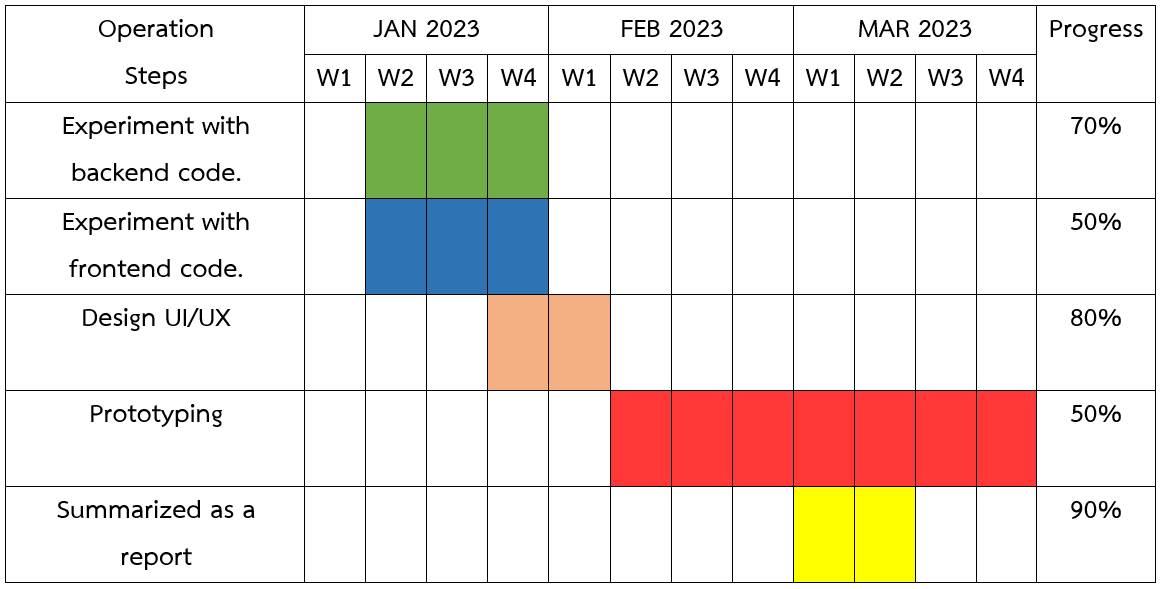
\includegraphics[width=\textwidth]{images/plan_progress.png}
\end{figure}


\section{\ifenglish Roles and responsibilities\else บทบาทและความรับผิดชอบ\fi}
\begin{itemize}
    \item นายธนัตถ์ ตั้งอั้น รหัส 630610737 ทำในส่วนของ Backend โดยมีองค์ประกอบหลักๆ ก็คือตัวเว็บเซิฟเวอร์, database, การคำนวณ fuzzy logic และตัวชี้วัดทางเทคนิคต่างๆ และ
การปรับแต่ง fuzzy logic ด้วย PSO
    \item นายธนวัตน์ บำเพ็งพันธุ์ รหัส 630610736 ทำในส่วนของ Frontend คือการออกแบบ UI/UX, สร้างเว็บและแอปพลิเคชันมือถือเพื่อติดต่อกับ User และบริการเว็บเซิฟเวอร์
\end{itemize}
% นายธนัตถ์ ตั้งอั้น รหัส 630610737 ทำในส่วนของ Backend โดยมีองค์ประกอบหลักๆ ก็คือตัวเว็บเซิฟเวอร์, database, การคำนวณ fuzzy logic และตัวชี้วัดทางเทคนิคต่างๆ และ
% การปรับแต่ง fuzzy logic ด้วย PSO
% นายธนวัตน์ บำเพ็งพันธุ์ รหัส 630610736 ทำในส่วนของ Frontend คือการออกแบบ UI/UX, สร้างเว็บและแอปพลิเคชันมือถือเพื่อติดต่อกับ User และบริการเว็บเซิฟเวอร์

\section{\ifenglish%
Impacts of this project on society, health, safety, legal, and cultural issues
\else%
ผลกระทบด้านสังคม สุขภาพ ความปลอดภัย กฎหมาย และวัฒนธรรม
\fi}
ระบบนี้อาจจะสามารถต่อเติมด้วยการใส่ตัวชี้วัดทางเทคนิคอื่นๆ ที่อาจจะมาจากแหล่งต่างๆมาเพื่มความละเอียดในการวิเคราะห์บางอย่าง
ซึ่งถ้าระบบนี้สำเร็จ ระบบนี้อาจจะเป็นเครื่องมือสำคัญให้กับนักลงทุนหลายๆคน และสามารถช่วยสร้างกำไรให้นักลงทุนเพิ่มได้ 
\chapter{\ifenglish Background Knowledge and Theory\else ทฤษฎีที่เกี่ยวข้อง\fi}

การทำโครงงาน เริ่มต้นด้วยการศึกษาค้นคว้า ทฤษฎีที่เกี่ยวข้อง หรือ งานวิจัย/โครงงาน ที่เคยมีผู้นำเสนอไว้แล้ว ซึ่งเนื้อหาในบทนี้ก็จะเกี่ยวกับการอธิบายถึงสิ่งที่เกี่ยวข้องกับโครงงาน เพื่อให้ผู้อ่านเข้าใจเนื้อหาในบทถัดๆ ไปได้ง่ายขึ้น

\section{ตรรกศาสตร์คลุมเครือ (Fuzzy Logic)}
ตรรกศาสตร์คลุมเครือ เป็นแนวคิดเกี่ยวกับการวิเคราะห์เชิงตรรกะ แต่การวิเคราะห์ไม่ได้มีเพียง ถูกกับผิด หรือ 0 กับ 1 เนื่องจากเหตุการณ์ในความเป็นจริงสร้างความคลุมเครือในการวิเคราะห์ เช่น อุณหภูมิอากาศ 20 องศาเซลเซียสเป็นอากาศที่หนาวไปหรือไม่? หากนำคำถามนี้ไปให้ผู้วิเคราะห์ต่างที่อยู่อาศัยกัน จะได้คำตอบที่ไม่เหมือนกัน เนื่องจากการวิเคราะห์แนวนี้ไม่เหมาะกับการตอบเพียงใช่หรือไม่ การใช้ตรรกศาสตร์คลุมเครือ (Fuzzy Logic) มาใช้วิเคราะห์เหตุการณ์จึงจะได้คำตอบที่ดีกว่า แทนที่จะตอบเพียงแค่ ใช่หรือไม่ คำตอบที่ได้จะเป็นพจน์ของ ตัวแปรทางภาษา (Linguistic Variable) และความเป็นสมาชิก เช่นตัวแปรทางภาษาอุณหภูมิมีค่า หนาว 60\% อบอุ่น 15\% ร้อน 0\% (เพราะผู้วิเคราะห์อาจจะรู้สึกหนาวแต่ก็ไม่ได้หนาวเกินไปหรืออบอุ่นอยู่เล็กน้อย) จะเห็นว่าการบอกค่าเชิงตรรกะแบบฟัซซีสะท้อนความจริงได้ดีกว่าการตอบแบบเดิม

% \section{Second section}
% Section 2 text.

\subsection{ฟัซซีเซต (Fuzzy Set)}
เป็นเซตที่ขอบเขตไม่เด่นชัดหรือคลุมเครือโดยการบอกค่าเชิงตรรกะจะถูกสร้างเป็นฟัซซีเซตที่เราสามารถวัดระดับความเป็นสมาชิก (Membership Value) ของสมาชิกในเอกภพสัมพัทธ์ต่อฟัซซีเซตนั้นผ่านทางฟังก์ชันภาวะสมาชิก (Membership function) ซึ่งเป็นฟังก์ชันที่รับสมาชิกในเอกภพสัมพัทธ์แล้วส่งไปที่ช่วง [0,1] โดยจากตัวอย่างดังกล่าวจะสามารถสร้างเป็นฟัซซีเซ็ตได้เป็น เซ็ตของอากาศ เย็น, อบอุ่น, ร้อน โดยให้อุณหภูมิเป็นสมาชิกของเซ็ตซึ่งสมาชิกแต่ละตัวสามารถเป็นสมาชิกของทุกเซ็ตได้ เช่น อุณหภูมิ 20 องศาเซลเซียส มีระดับความเป็นสมาชิกในฟัซซีเซตอากาศเย็น 0.6, อบอุ่น 0.15, ร้อน 0
\begin{figure}[ht]
    \centering
    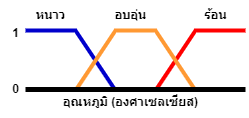
\includegraphics[scale=0.7]{images/fuzzy_set.png}
    \caption{ฟัซซีเซต หนาว,อบอุ่น,ร้อน และฟังก์ชันภาวะสมาชิก}
    \label{fig:1}
\end{figure}

\subsection{ระบบประมวลผลตรรกศาสตร์คลุมเครือ (Fuzzy Logic System)}
เป็นการนำเอาความสามารถของตรรกศาสตร์คลุมเครือมาสร้างเป็นระบบประมวลผลแบบตรรกศาสตร์คลุมเครือซึ่งเป็นการเลียนแบบการคิด การหาเหตุผล การตัดสินใจและการกระทำของมนุษย์ โดยจะมีส่วนประกอบสำคัญ 4 ส่วนคือ 1. การแปลงข้อมูลขาเข้าเป็นฟัซซี (Fuzzification), 2. กฏ (Fuzzy Rules), 3. การอนุมานหรือการตีความ (Inference), 4. การแปลงข้อมูลฟัซซีเป็นตัวเลข (Defuzzification)
ซึ่งจะมีตัวอย่างการทำงานเมื่อใช้ระบบประมวลผลตรรกศาสตร์คลุมเครือดังภาพรวมนี้
\begin{figure}[ht]
    \centering
    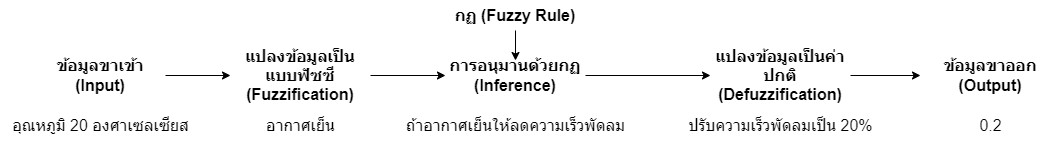
\includegraphics[scale=0.375]{images/ex_fis.png}
    \caption{ตัวอย่างการทำงานของระบบประมวลผลตรรกศาสตร์คลุมเครือ}
    \label{fig:2}
\end{figure}

โดยในงานนี้เราใช้ระบบฟัซซีแบบ Mamdani

\subsubsection{การแปลงข้อมูลขาเข้าเป็นฟัซซี (Fuzzification)}
เป็นการแปลงข้อมูลอินพุตทั่วไปที่เป็นตัวเลข (Crisp Set) ไปเป็นข้อมูลในรูปแบบฟัซซีเซต หรือที่เรียกว่าตัวแปรทางภาษา (Linguistic Variable) โดยจะสร้างฟังก์ชันภาวะสมาชิกซึ่งขึ้นอยู่กับลักษณะของข้อมูลขาเข้าและความสำคัญต่อข้อมูลเอาท์พุต
\begin{equation} \mu_A(x) = \begin{cases}
0 & \text{if } x \leq a \\
\frac{x-a}{b-a} & \text{if } a < x < b \\
\frac{c-x}{c-b} & \text{if } b \leq x < c \\
0 & \text{if } x \geq c \\
\end{cases} \end{equation}
\begin{figure}[ht]
    \centering
    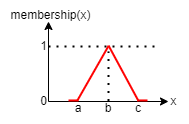
\includegraphics[scale=0.7]{images/ex_memship.png}
    \caption{ตัวอย่างกราฟฟังก์ชันภาวะสมาชิก Triangular function}
    \label{fig:3}
\end{figure}

\subsubsection{กฏฟัซซี (Fuzzy Rules) \cite{Sansanee}}
เป็นส่วนของการกำหนดวิธีการควบคุมซึ่งได้มาจากผู้เชี่ยวชาญหรือการปรับแต่งทดลองขึ้นเองโดยจะอยู่ในรูปแบบของชุดข้อมูลแบบกฏของภาษา ซึ่งกฏฟัซซีแบบที่นิยมใช้มากและใช้ในงานนี้เป็นกฏฟัซซีแบบ ถ้า-แล้ว (If-then rule)
โดยในงานนี้ได้ใช้วิธีการของ Mamdani หากมีอินพุต \(X_{1},X_{2},...,X_{n}\) และพจน์ภาษา \(T(x_{i})\) ของตัวแปรทางภาษา \(x_{i}\) ในเซตสากล \(X_{i}\) สำหรับ \(1 \le i \le n\) ในขณะเดียวกัน \(Y\) ก็ถูกนิยามด้วยตัวแปรทางภาษา และพจน์ภาษา \(T(y)\) ของตัวแปรทางภาษา y ในเซตสากล \(Y\)
\[ IF\; x_{1}\; is\; A^{(1)}\; and\; x_{2}\; is\; A^{(2)}\; and\; ... \; and\; x_{n}\; is\; A^{(n)}\; THEN\; y\; is\; B \]
โดยที่ \(A^{(1)},A^{(2)},...,A^{(n)}\) เป็นพจน์ในภาษา \(T(x_{i})\) และ B เป็นพจน์ในภาษา \(T(y)\)

\subsubsection{การอนุมานหรือการตีความ (Inference) \cite{Sansanee}}
เป็นส่วนของการประมวลผลจะมีการตีความตามเงื่อนไขที่กำหนดไว้ หรือก็คือตีความผ่านกฏฟัซซี ซึ่งจากกฏฟัซซีดังกล่าวจะประกอบด้วยกันสองส่วนคือ ส่วนที่เกิดขึ้นก่อน (If Part) และผลที่ตามมา (Then part) โดยที่อินพุตและเอาท์พุตนั้นอาจมีหลายตัวก็ได้ขึ้นอยู่กับการออกแบบ ผลที่ตามมาของแต่ละกฏจะถูกรวมกันด้วยวิธีทางตรรกศาสตร์เพื่อให้ได้ค่าเอาท์พุตเพียงค่าเดียว

โดยจะเริ่มจากการหาระดับความเข้ากันได้ของแต่ละอินพุต \((x_{i}, i \in \{1,2,...,n\})\) กับพจน์ภาษาในกฏนั้น และเนื่องจากลักษณะของส่วนที่เกิดขึ้นก่อน (If Part) ของกฏต้องการให้ทุกอินพุตเป็นไปตามพจน์ภาษา ดังนั้นค่าความเป็นสมาชิกของแต่ละอินพุตในแต่ละพจน์ภาษาจะถูกรวมกันในลักษณะของตัวเชื่อม conjunction นั่นคือที่กฏ j
\begin{equation}
\alpha_{j} = min\{A^{(1)}_{i1,j}(x_{1}), A^{(2)}_{i2,j}(x_{2}), ..., A^{(n)}_{in,j}(X_{n})\}
\end{equation}
และเอาต์พุตของกฏ j เป็นฟัซซีเซตที่เกิดจากการตัด (cut off) พจน์ภาษา \(B_{i,j}\) ด้วย \(\alpha_{j}\) หรือ
\begin{equation}
OUT^{(j)}_{x_{1},x_{2},...,x_{n}} (y) = min(A^{(1)}_{i1,j}(x_{1}), A^{(2)}_{i2,j}(x_{2}),...,A^{(n)}_{in,j}(x_{n}),B_{i,j}(y))
\end{equation}
และเมื่อได้เอาต์พุตของแต่ละกฏแล้ว ฟัซซีเอาต์พุตจากทุกกฏจะถูกรวมกันโดยการหาฟัซซียูเนียนมาตรฐาน (ซึ่งจะได้ฟัซซีเอาต์พุตรวม (OUT)) สมมติให้มีกฏทั้งหมด k กฏ จะได้ OUT เป็น
\begin{equation}
OUT_{x_{1},x_{2},...,x_{n}} (y) = max_{j \in \{1,2,...,k\}}\; min(A^{(1)}_{i1,j}(x_{1}), A^{(2)}_{i2,j}(x_{2}),...,A^{(n)}_{in,j}(x_{n}),B_{i,j}(y))
\end{equation}
ตัวอย่าง สมมติให้ระบบมีกฏ 2 กฏ โดยที่แต่ละกฏจะมีอินพุต 2 อินพุต และแต่ละอินพุตในแต่ละกฏมีพจน์ภาษาดังรูป โดยที่มีกฏดังนี้คือ
\[R1:\; IF\; x_{1}\; is\; L_{1}\; and\; x_{2}\; is\; H_{2},\; THEN\; y\; is\; L \]
\[R2:\; IF\; x_{1}\; is\; M_{1}\; and\; x_{2}\; is\; M_{2},\; THEN\; y\; is\; H \]
ถ้ากำหนดให้ \(x_{1}\) มีค่าเท่ากับ 2 และ \(x_{2}\) มีค่าเท่ากับ 5 จะได้ว่า
\[\alpha_{1} = min(L_{1}(x_{1}),H_{2}(x_{2})) = min (1,0.5) = 0.5\]
\[\alpha_{2} = min(M_{1}(x_{1}),H_{2}(x_{2})) = min (0,0.5) = 0\]ฟัซซีเอาต์พุตของกฏที่ 1 และ 2 และฟัซซีเอาต์พุตรวม (OUT) แสดงในรูปดังนี้
\begin{figure}[ht]
    \centering
    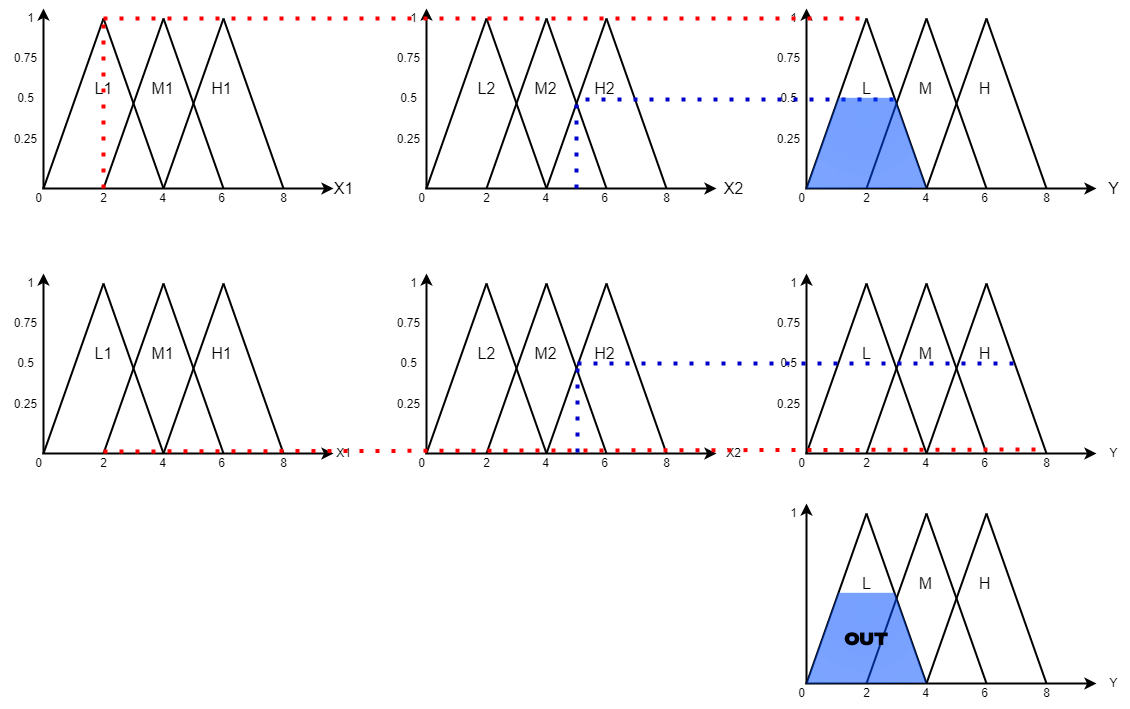
\includegraphics[scale=0.3]{images/ex_inference.png}
    \caption{ตัวอย่างการอนุมาน}
    \label{fig:4}
\end{figure}

\subsubsection{การแปลงข้อมูลฟัซซีเป็นค่าปกติ (Defuzzification)}
เนื่องจากผลลัพธ์ที่ได้จากการตีความนั้นยังอยู่ในรูปแบบของฟัซซี ในส่วนนี้เป็นการทำการแปลงข้อมูลที่อยู่ในรูปแบบฟัซซีเป็นข้อมูลที่เป็นตัวเลข (Crisp set) ด้วยวิธีทางคณิตศาสตร์ เช่น Center of Area (Centroid) เพื่อนำค่าที่ได้มาใช้ในการตัดสินใจและนำไปควบคุมระบบได้

วิธีแปลงโดยการหา Centroid จะหาค่าเอาต์พุตจากจุดศูนย์กลางของพื้นที่กราฟได้ดังสมการนี้
\begin{equation}
  de_y = \frac{\int B(z)\cdot zdz}{\int B(z)dz}
\end{equation}

โดย \(B(z)\) คือ ค่าความเป็นสมาชิก (Membership Value) ของตำแหน่ง \(z\)

\section{การหาค่าที่เหมาะสมที่สุดโดยกลุ่มของอนุภาค (Particle Swarm Optimization (PSO)) \cite{Sansanee}}
การหาค่าที่เหมาะสมที่สุดโดยกลุ่มของอนุภาค เป็นอัลกอริทึมการค้นหาที่ขึ้นกับประชากร ซึ่งเป็นการจำลองพฤติกรรมเชิงสังคมของฝูงนก ท่าทางของฝูงนกเชิงภูมิศาสตร์ที่คาดเดาไม่ได้ โดยที่มีจุดประสงค์ในการค้นพบรูปแบบที่ควบคุมความสามารถของนกในการบินพร้อมกันและสามารถเปลี่ยนทิศทางได้อย่างกะทันหัน โดยการรวมกลุ่มกันใหม่ในลักษณะที่เหมาะสมที่สุด ทำให้เกิดอัลกอริทึมสำหรับการจัดระเบียบกลุ่มของอนุภาค ที่ง่ายและมีประสิทธิภาพ

\subsection{อนุภาค (Particle)}
อนุภาค 1 อนุภาค คือคำตอบที่เป็นไปได้ของปัญหาการหาค่าที่เหมาะสม โดยอนุภาคจะบินในปริภูมิการค้นหาหลายมิติ การเปลี่ยนแปลงของอนุภาคในกลุ่มนั้นมีอิทธิพลมาจากประสบการณ์ หรือความรู้ของเพื่อนบ้าน รูปร่างของเพื่อนบ้านมีหลายรูปแบบ และมีการสร้างอัลกอริทึมตามแต่ละรูปแบบ

\subsubsection{ทอพอโลยีแบบดาว (Star Topology)}
รูปแบบนี้ทำให้แต่ละอนุภาคสามารถติดต่อกับอนุภาคอื่นได้ทุกอนุภาค แต่ละอนุภาคจะสนใจอนุภาคที่ดีที่สุดในกลุ่ม และแต่ละอนุภาคจะเลียนแบบอนุภาคที่ดีที่สุดในกลุ่มนี้เอง โดยอัลกอริทึมที่จำลองสถานการณ์นี้คือ อัลกอริทึมดีที่สุดแบบรวม (global best)
\begin{figure}[ht]
    \centering
    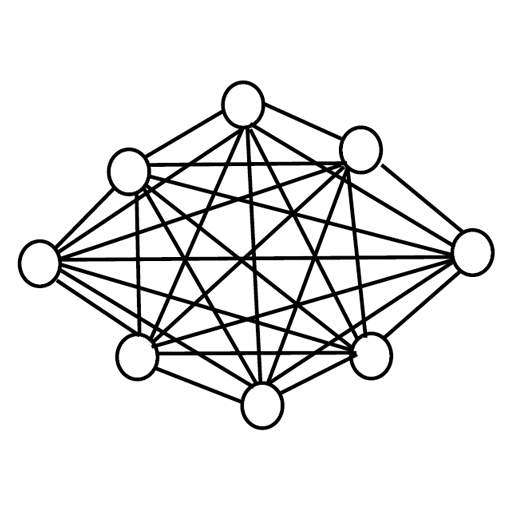
\includegraphics[scale=0.3]{images/star_topology.png}
    \caption{รูปแบบของเพื่อนบ้านสำหรับการจัดระเบียบกลุ่มของอนุภาค ทอพอโลยีแบบดาว}
    \label{fig:5}
\end{figure}

\subsubsection{ทอพอโลยีแบบวงแหวน (Ring Topology)}
รูปแบบนี้ทำให้แต่ละอนุภาคจะติดต่อได้กับเพื่อนบ้านที่ใกล้ที่สุด \(n\) อนุภาค ดังแสดงในรูป เมื่อ \(n=2\) ดังนั้นอนุภาคเคลื่อนที่ตามเพื่อนดีที่ในกลุ่มเพื่อนบ้านที่ติดต่อได้ ซึ่งอัลกอริทึมที่จำลองสถานการณ์นี้คือ อัลกอริทึมดีที่สุดแบบเฉพาะที่ (local best)
\begin{figure}[ht]
    \centering
    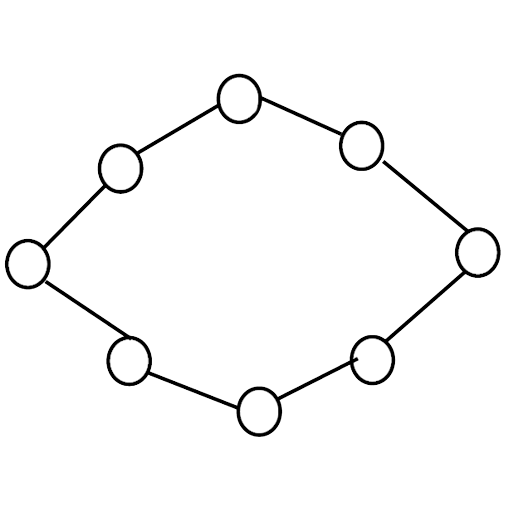
\includegraphics[scale=0.3]{images/ring_topology.png}
    \caption{รูปแบบของเพื่อนบ้านสำหรับการจัดระเบียบกลุ่มของอนุภาค ทอพอโลยีแบบวงแหวน}
    \label{fig:6}
\end{figure}

\subsection{อัลกอริทึมสำหรับการจัดระเบียบกลุ่มของอนุภาค}
อนุภาคจะบินอยู่ในปริภูมิการค้นหาหลายมิติ โดยที่ตำแหน่งของอนุภาคจะเปลี่ยนไปตามประสบการณ์ของตัวอนุภาคเอง หรือของเพื่อนบ้าน ให้ \(x_{i}(t)\) เป็นตำแหน่งของอนุภาค \(P_{i}\) ในปริภูมิไฮเปอร์ (hyperspace) ที่เวลา \(t\) และตำแหน่งของอนุภาคจะเปลี่ยนได้โดยการเพิ่มความเร็ว \(v_{i}(t)\) ให้กับตำแหน่งปัจจุบันดังนี้
\begin{equation}
  x_{i}(t) = x_{i}(t-1)+v_{i}(t)
\end{equation}
ซึ่งความเร็วนี้เป็นตัวขับในกระบวนการหาค่าที่เหมาะสม และสะท้อนถึงการแลกเปลี่ยนข้อมูลในสังคม
\subsubsection{ฟังก์ชันจุดประสงค์ (Objective Function)}
เป็นฟังก์ชันที่เราสร้างขึ้นมาหรือฟังก์ชันปัญหาที่เราต้องการหาค่าที่เหมาะสมที่สุดเพื่อที่จะทำให้ได้คำตอบที่ดีที่สุด และจะใช้คำนวณหาค่าความเหมาะสม ซึ่งเปรียบเหมือนประสิทธิภาพของแต่ละอนุภาค

\subsubsection{อัลกอริทึมดีที่สุดแบบรวม (Global Best)}
อัลกอริทึม gbest นี้เป็นการใช้โครงสร้างทอพอโลยีแบบดาว ดังนั้นการเคลื่อนที่ของอนุภาคจะขึ้นอยู่กับตำแหน่งที่ดีที่สุดของอนุภาคตัวที่ดีที่สุดในกลุ่ม และประวัติจากประสบการณ์ของตนเอง ดังนั้นอัลกอริทึมนี้สามารถสรุปได้ดังนี้
\begin{enumerate}
\item ตั้งค่ากลุ่ม (P(t) ที่ t=0) ของอนุภาค โดยที่ตำแหน่ง \((x_{i}(t))\) ของอนุภาค \(i (P_{i} \in P(t))\) จะถูกสุ่มโดยให้ค่าอยู่ภายในปริภูมิไฮเปอร์ ที่ต้องการค้นหาคำตอบ
\item คำนวณค่าประสิทธิภาพ \(F\) ของแต่ละอนุภาค โดยใช้ตำแหน่งปัจจุบัน \(x_{i}(t)\)
\item เปรียบเทียบค่าที่ได้ในข้อ 2 ของอนุภาค \(i\) กับค่าที่ดีที่สุดของตนเอง \((pbest_{i})\) ดังนี้ ถ้า \(F(x_{i}(t)) < pbest_{i}\) แล้วกำหนดให้ \(pbest_{i} = F(x_{i}(t))\) และ \(x_{pbest_{i}}(t) = x_{i}(t)\)
\item เปรียบเทียบค่าที่ได้ในข้อ 2 ของอนุภาค \(i\) กับค่าที่ดีที่สุดของกลุ่ม \((gbest)\) ดังนี้ ถ้า \(F(x_{i}(t)) < gbest\) แล้วกำหนดให้ \(gbest = F(x_{i}(t))\) และ \(x_{gbest}(t) = x_{i}(t)\)
\item ปรับความเร็วของแต่ละอนุภาคดังนี้ \begin{equation}
  v_{i}(t) = v_{i}(t-1) + \rho_{1}(x_{pbest_{i}} - x_{i}(t)) + \rho_{2}(x_{gbest} - x_{i}(t))
\end{equation} โดยที่ \(\rho_{1}\) และ \(\rho_{2}\) เป็นค่าที่ถูกสุ่มมา
\item ปรับตำแหน่งของแต่ละอนุภาค ตามสมการที่ 2.6 และตั้งค่า \(t = t+1\)
\item กลับไปยังข้อ 2 และทำซ้ำ จนกระทั่งจะลู่เข้า (converge)
\end{enumerate}

\subsubsection{อัลกอริทึมดีที่สุดแบบเฉพาะที่ (Local Best)}
อัลกอริทึม lbest นี้เป็นการใช้เพื่อนบ้านในลักษณะของทอโพโลยีแบบวงแหวน ดังนั้นอนุภาคที่มีผลต่อการเคลื่อนที่คืออนุภาคที่อยู่ในเพื่อนบ้าน ที่ดีที่สุดและตำแหน่งที่ดีที่สุดของตนเอง ซึ่งอัลกอริทึมนี้จะคล้ายกับแบบ gbest เพียงแต่ในขั้นตอนที่ 4 และ 5 เปลี่ยนจาก gbest เป็น lbest นั่นเอง

อัลกอริทึม lbest นี้จะช้าในการลู่เข้ามากกว่าแบบ gbest แต่จะให้คำตอบที่ดีกว่า และเป็นการค้นหาโดยครอบคลุมพื้นที่ได้กว้างกว่า

\section{\ifenglish%
\ifcpe CPE \else ISNE \fi knowledge used, applied, or integrated in this project
\else%
ความรู้ตามหลักสูตรซึ่งถูกนำมาใช้หรือบูรณาการในโครงงาน
\fi
}

ทฤษฎีตรรกศาสตร์คลุมเครือ และการหาคำตอบที่เหมาะสมแบบฝูงอนุภาค ทั้ง 2 ทฤษฎีนี้เป็นสิ่งที่เราได้เรียนรู้มาจากวิชา Introduction to Computational Intelligence for Computer Engineering (261456) โดยในงานนี้เราได้นำทั้ง 2 ทฤษฎีมาใช้งานร่วมกันโดยใช้ทฤษฎีการหาคำตอบที่เหมาะสมแบบฝูงอนุภาคในการปรับพารามิเตอร์ในระบบประมวลผลฟัซซี

\section{\ifenglish%
Extracurricular knowledge used, applied, or integrated in this project
\else%
ความรู้นอกหลักสูตรซึ่งถูกนำมาใช้หรือบูรณาการในโครงงาน
\fi
}

ความรู้เกี่ยวกับการเทรด การใช้งานและวิเคราะห์ตัวชี้วัดทางเทคนิค

\chapter{\ifproject%
      \ifenglish Project Structure and Methodology\else โครงสร้างและขั้นตอนการทำงาน\fi
  \else%
      \ifenglish Project Structure\else โครงสร้างของโครงงาน\fi
  \fi
 }

ในบทนี้จะกล่าวถึงหลักการ, การนำทฤษฎีที่เกี่ยวข้องมาประยุกต์ใช้ และการออกแบบของระบบ

\makeatletter

% \renewcommand\section{\@startsection {section}{1}{\z@}%
%                                    {13.5ex \@plus -1ex \@minus -.2ex}%
%                                    {2.3ex \@plus.2ex}%
%                                    {\normalfont\large\bfseries}}

\makeatother
%\vspace{2ex}
% \titleformat{\section}{\normalfont\bfseries}{\thesection}{1em}{}
% \titlespacing*{\section}{0pt}{10ex}{0pt}

\section{การจัดเก็บข้อมูล}
โดยข้อมูลราคาหุ้นทุกตัวจะมีแหล่งที่มาจาก AlphaVantage โดยจะให้ข้อมูลย้อนหลังไป 2 ปี และใช้อัพเดท
ข้อมูลแบบทุกๆ 30 นาที และในส่วนของราคา Crypto-Currency จะมีแหล่งที่มาจาก Binance ทั้งหมดซึ่งมีการอัพเดททุกๆ 30 นาทีเช่นกัน
เราใช้ MongoDB เป็น Database สำหรับจัดเก็บข้อมูลตลาดหุ้น

ในตอนเริ่มตันนั้นเราดึงข้อมูลที่ต้องการมาจาก AlphaVantage API ซึ่งได้มาเป็นข้อมูลตลาดหุ้นย้อนหลัง 2 ปีโดย
และเก็บข้อมูลลง MongoDB โดยมีการแปลงข้อมูลให้เป็นในรูปแบบข้อมูลตลาดของเราซึ่งก็จะประกอบด้วย
\begin{enumerate}
    \item ticker: ชื่อของหุ้นที่ทำการซื้อขาย เช่น AAPL/USD, TSLA/USD, ETH/USDT
    \item open: เป็นราคาซื้อขายแรกที่เกิดขึ้นใน ช่วงเวลานั้นๆ
    \item close: เป็นราคาสุดท้ายที่เกิดขึ้นจากการซื้อขายสิ้นสุด ของช่วงเวลานั้นๆ
    \item high: การเคลื่อนไหวของราคาหุ้น ณ ระดับราคาสูงสุดในช่วงเวลานั้นๆ
    \item low: การเคลื่อนไหวของราคาหุ้น ณ ระดับราคาต่ำสุดในช่วงเวลานั้นๆ
    \item volume: ปริมาณการซื้อขายในช่วงเวลานั้นๆ
\end{enumerate}
จากนั้นในการอัพเดตข้อมูลทุกๆ 30 นาที เราจะใช้ Amazon EventBridge Scheduler ที่จะไปเรียกใช้ AWS Lambda ที่เราสร้างขึ้นมาโดยใน Lambda จะดึงข้อมูลจาก
AlphaVantage มาอัพเดต ในส่วนของ Crypto-Currency ก็จะใช้ระบบแบบเดียวกันแต่จะใช้ Binance API ทั้งในการดึงข้อมูลครั้งแรกและการอัพเดตแทน

\begin{figure}[ht]
    \centering
    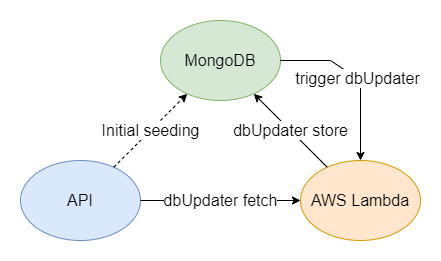
\includegraphics[scale=0.6]{images/db.png}
    \caption{โครงสร้างของการจัดเก็บข้อมูล โดนเส้นประคือทำครั้งเดียวในตอนแรกเริ่ม และเส้นทึบจะทำในทุกๆ ชม. โดยเป็นการเรียกใช้โปรแกรม dBUpdater ใน AWS Lambda}
    \label{fig:7}
\end{figure}
\FloatBarrier

\section{การสร้างตัวชี้วัดทางเทคนิคด้วย Fuzzy Logic}
เราจะใช้ Mamdani Fuzzy Inference System กับตัวแปรทางภาษาและ Fuzzy Rule ที่จะกล่าวด้านล่างนี้ในการคำนวณค่าสัญญาณของเรามา โดย defuzzification method จะใช้แบบ
centroid

\subsection{ตัวแปรทางภาษา (Linguistic Variable)}
สำหรับตัวชี้วัดทางเทคนิคแต่ละตัวที่เรามีให้ได้แก่ Relative Index Strength (RSI), Bollinger Band (BB), Moving Average Convergence/Divergence
(MACD), Average Directional Index (ADX), Aroon oscillator (AROON), On-Balance Volume (OBV), Stochastic Oscillator,
Accumulation/Distribution Indicator (A/D) ซึ่งผู้ใช้สามารถใช้ระบบของเราผ่านเว็บแอปพลิเคชัน ในการสร้างตัวแปรทางภาษาจากแต่ละตัวชี้วัดทางเทคนิค
และก็สามารถสร้างตัวแปรทางภาษาสำหรับสัญญาที่จะออกมายกตัวอย่างเช่น ทำป็นสัญญาณ long (ควรเข้า position long) และสัญญาณ short (ควรเข้า position short)
ซึ่งจะคิดมาจากตัวแปรทางภาษาของตัวชี้วัดทางเทคนิคที่กล่าวถึงด้านบน ยกตัวอย่างตัวแปรทางภาษาที่เราอาจจะใช้บนรูปที่ \ref{fig:8}
\begin{figure}[ht]
    \centering
    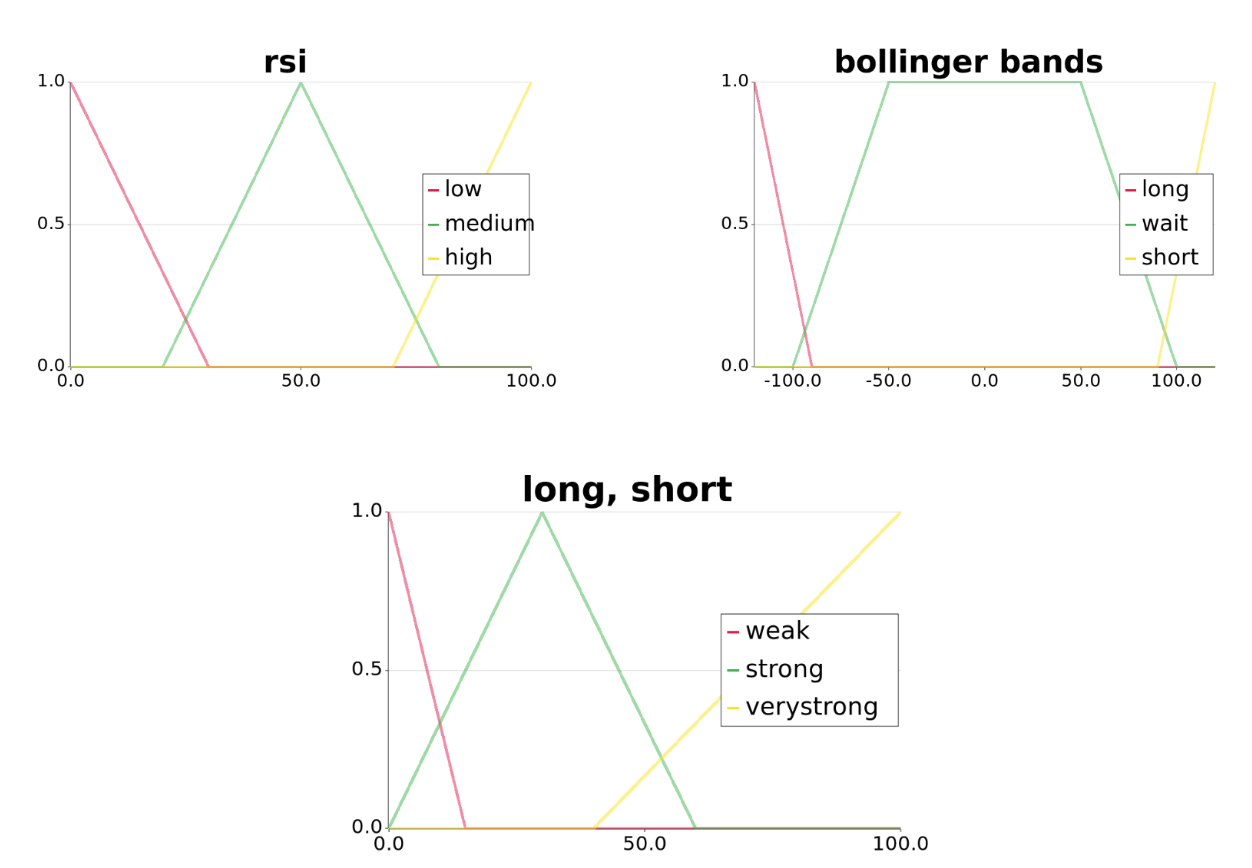
\includegraphics[width=\textwidth]{images/linguistic.png}
    \caption{ตัวแปรทางภาษาสำหรับ RSI, Bollinger Band, long, short}
    \label{fig:8}
\end{figure}

\subsection{Fuzzy Rules}
เราจะใช้การตีความทั่วๆไปของแต่ละตัวชี้วัดมาสร้าง Fuzzy Rule เริ่มต้น ยกตัวอย่างเช่นถ้าเราใช้แค่ RSI และ Bollinger Band ในการสร้าง long และ short เราจะมี fuzzy rule
เหมื่อนในตารางที่ \ref{table:1} โดยในระบบของเราจริงๆ เราจะใช้ตัวแปรทางภาษาที่เรากล่าวในหัวข้อก่อนหน้ามาทั้งหมดสร้าง Fuzzy Rule ในการสร้างสัญญาณ long และ short และเรา
จะออกแบบระบบให้ผู้ใช้สามารถปรับแต่งกฏตรงนี้ได้ในทั้ง website

\begin{table}[htp]
    \centering
    \begin{tabular}{c c c c}
        \toprule
        {RSI}  & {Bollinger Bands} & {LONG}     & {SHORT}    \\
        \midrule
        HIGH   & LONG              & WEAK       & WEAK       \\
        HIGH   & WAIT              & WEAK       & STRONG     \\
        HIGH   & SHORT             & WEAK       & VERYSTRONG \\
        MEDIUM & LONG              & WEAK       & STRONG     \\
        MEDIUM & WAIT              & WEAK       & WEAK       \\
        MEDIUM & SHORT             & STRONG     & WEAK       \\
        LOW    & LONG              & VERYSTRONG & WEAK       \\
        LOW    & WAIT              & STRONG     & WEAK       \\
        LOW    & SHORT             & WEAK       & WEAK       \\
        \bottomrule
    \end{tabular}
    \caption{ตัวอย่างของ Fuzzy Rules ที่ใช้แค่ RSI และ Bollinger Band เพื่อสร้าง long และ short.}
    \label{table:1}
\end{table}
\FloatBarrier

\section{การปรับแต่ง Fuzzy Logic ด้วย PSO}
เป้าหมายของเราในการปรับแต่ง Fuzzy Logic ที่ใช้สำหรับการสร้างตัวชี้วัดทางเทคนิคใหม่ของเรานั้น ก็คือการปรับแต่งตัวแปรทางภาษาต่างๆ ที่มีอยู่ fuzzy rules เพื่อให้
ตัวชี้วัดทางเทคนิคของเรานั้นสามารถสร้างกำไรได้มากที่สุดใน\emph{วิธีการเทรดที่เราใช้ปรับแต่ง} โดยเราจะใช้ PSO (Particle Swarm Optimization) ในการปรับพารามิเตอร์ที่ใช้
สร้างตัวแปรทางภาษาแต่ละอัน โดยพารามิเตอร์ในการสร้าง fuzzy set นั้นจะแตกต่างกันไปตามรูปแบบของ fuzzy set
เช่นถ้าเป็นแบบสามเหลี่ยมก็จะมีพารามิเตอร์ดังที่เห็นในรูปที่ \ref{fig:9} โดยผู้ใช้งานจะสามารถใช่ PSO ในการปรับแต่งตัวแปรทางภาษาได้เองผ่าน website ที่เราจัดทำขึ้นมา

\begin{figure}[ht]
    \centering
    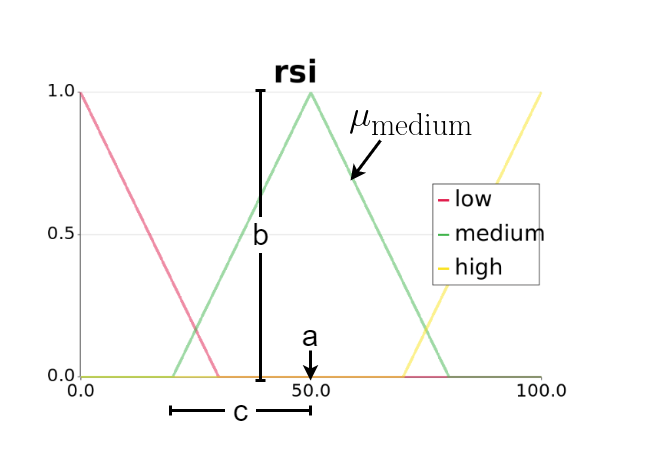
\includegraphics[width=0.8\textwidth]{images/linguisticv.png}
    \caption{ตัวแปรทางภาษาและตัวแปรที่เราต้องการจะปรับแต่ง $\mu_{\text{medium}} = b (1 - \frac{ |x-a| }{s})$ (ในที่นี้คือเราจะปรับแต่งค่าของ $a, b, s$)}
    \label{fig:9}
\end{figure}

\subsection{กลยุทธ์ที่เราใช้ปรับแต่ง}
โดยในการปรับแต่ง Fuzzy Logic ของเรานั้นอันดับแรกเลยเราต้องเลือกกลยุทธ์การเทรดที่เราต้องการปรับแต่ง ให้มีผลต่อตัวชี้วัดทางเทคนิค ยกตัวอย่างกลยุทธ์การเทรด
เช่น มีเงินต้น 2000 บาท ถ้า buySignal มากกว่า 50 ให้เข้าซื้อด้วย 100 บาท ด้วย stop-loss ที่ 10\% และ take profit ที่ 20\%
\subsection{Backtesting}
Backtesting คือการนำกลยุทธ์การเทรดที่เราเลือก ไปใช้กับข้อมูลในอดีตในกรอบเวลาที่ผ่านๆ มาเพื่อทดสอบว่ากลยุทธ์นั้นไปใช้ในตลาดจริงๆ ในอดีตแล้วได้ผลดีแค่ไหน
โดยเราสามารถเลือกกรอบเวลาที่ตลาดมีลักษณะคล้ายๆ กับในปัจจุบัน แล้วลองปรับเปลี่ยนและทดสอบกลยุธ์การเทรดนั้นๆ ได้เพื่อให้ได้ผลลัพธ์ที่เราต้องการ

โดยเราจะทำการ backtest ด้วยกลยุทธ์การเทรดที่เราเลือกมา แล้วเก็บข้อมูลการเทรดที่เกิดขึ้นทั้งหมดโดยแต่ละการเทรดจะมีข้อมูลดังนี้
\begin{itemize}
    \item เวลาที่เข้า position
    \item เวลาที่ออก position
    \item ราคาที่เข้าซื้อ
    \item ราคาที่ขาย
    \item จำนวนเงินที่จ่ายไป
    \item กำไรขาดทุนที่ได้ ($\text{realizedPnl}$)
\end{itemize}

\subsection{Objective Function}
เราจะใช้ Objective Function ที่คำนวณมาดังนี้ 
$$ f = 
\begin{cases}
    \infty & |\text{trades}| = 0 \\
    -1 \times ((\text{np} - \text{np}_r) + (\text{mdd}_r - \text{mdd})) & \text{otherwise} \\ 
\end{cases}
$$ 
โดยที่
\begin{itemize}
    \item {$\text{np} = \frac{\sum_{i=0}^{n} p_i(\text{realizedPnl})}{\text{startMoney}}$
          คือ Net Profit ที่มีค่าอยู่ในช่วง $[0, \infty)$ ซึ่งได้จากการเทรดทั้งหมดโดยคำนวนจากข้อมูลการเทรดที่เราได้จากการทำ backtest โดย $n$ คือจำนวนข้อมูลทั้งหมด
          และ $p_i(\text{realizedPnl})$ คือข้อมูลตัวที่ $i$ โดยเอาค่า $\text{realizedPnl}$ มา
          }
    \item {$\text{mdd}$ (Maximum Drawdown ตัวอย่างในรูปที่ \ref{fig:10}) มีค่าอยู่ในช่วง $[0, 1]$ โดยเราสามารถคิดค่านี้โดยให้
          $$
              g(x) = \sum_{i = 0}^{x}p_i(\text{realizedPnl})
          $$
          \begin{equation}
              \text{mdd}' = \max_{r \in (0, n)} \left[ \max_{t \in (0, r)} g(t) - g(r) \right]
          \end{equation}
          แล้วให้เราจำค่า $y = g(t)$ ที่ทำให้ได้
          $\text{mdd}'$ เยอะที่สุดไว้ แล้วจะได้ว่า $\text{mdd} = \frac{\text{mdd}'}{y}$
          }
    \item {$|\text{trades}|$ คือจำนวนของการซื้อขายที่เกิดขึ้นในการ backtest}
    \item {$\text{np}_r$ และ  $\text{mdd}_r$ คือค่า Net Profit และ Maximum Drawdown ที่เราได้จากการ backtest โดยใข้ตัวแปรทางภาษาตั้งต้นก่อนที่จะทำการ
          ฝึกสอนด้วย PSO โดยเราจะใช้ค่านี้เป็นตัวอ้างอิงไว้เปรียนเทียบกับผลลัพธ์ของการปรับแต่งตัวแปรทางภาษาเพื่อให้เราได้ผลที่ไม่แย่ไปกว่าตัวแปรทางภาษาแบบเดิม
          }
\end{itemize}
ในส่วนของ hyper parameters ต่างๆ ที่เราต้องตั้งให้ PSO algorithm เช่น จำนวน particles, การคำนวณ velocity เป็นต้น จะเปลี่ยนไปตามแต่ละครั้งของการปรับแต่ง
โดยเราจะทดลองหลายๆ แบบเพื่อให้ได้ตัวชี้วัดที่มีประสิทธิภาพดีที่สุด

\begin{figure}[ht]
    \centering
    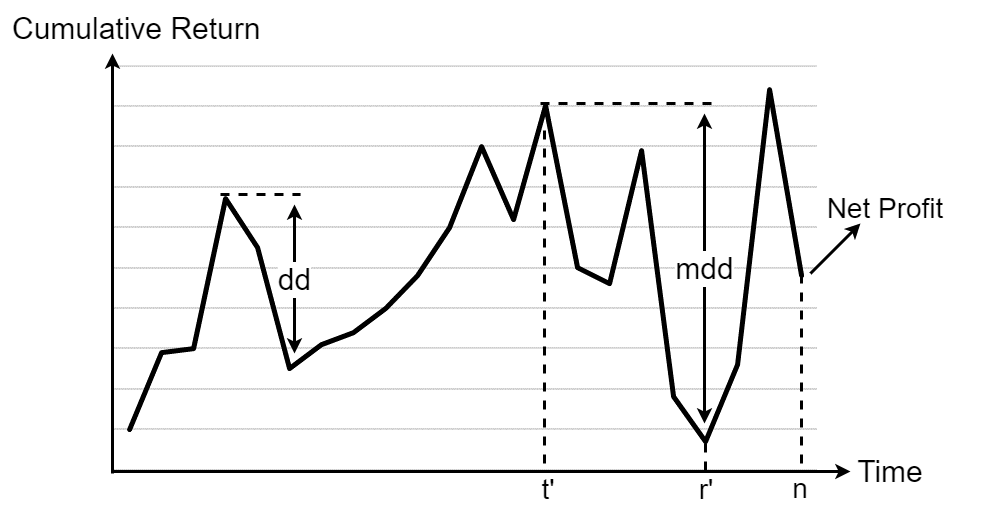
\includegraphics[width=0.8\textwidth]{images/mdd.png}
    \caption{ตัวอย่างของ Net Profit และ Maximum Drawdown}
    \label{fig:10}
\end{figure}

\section{การจัดการเงินทุน}
เราจะใช้ optimal-f (\cite{Vince}) ที่ถูกดัดแปลงตามที่ \cite{Rodrigo} ได้ทำไว้ในส่วนของการจัดการเงินทุน ซึ่งจะบอกเราว่าควรลงทุุนโดยใช้เงินเท่าไหร่ เพื่อให้เงินกำไรเติบโตแบบ
exponential โดยจะคิดมาจากผลลัพธ์ของการเทรดก่อนหน้า ถ้าเราเทรดสำเร็จเยอะก็จะเพิ่มเงินที่จะลงทุน ถ้าเทรดพลาดเยอะก็จะลดเงินที่จะลงทุน

อันดับแรกให้เราหาค่า $f$ ที่ทำให้ terminal wealth relative ($\text{TWR}$) ในสมการ \ref{eq:twr} มีค่ามากที่สุด
\begin{equation}
    \text{TWR}(f) = \Pi_{i=1}^{n} \text{HPR}_i(f)
    \label{eq:twr}
\end{equation}
\begin{equation}
    \text{HPR}_i(f) = 1 + \frac{f \cdot p_i(\text{realizedPnl})}{\text{riskFactor}}
\end{equation}
โดยที่ $\text{HPR}$ คือ holding perioid return หรือก็คืออัตราส่วนกำไรขาดทุนของแต่ละ position
,$n$ คือจำนวน position ทั้งหมด, $p_i(\text{realizedPnl})$ คือกำไรขาดทุนของ position ที่ $i$,
และ $\text{riskFactor}$ คือค่าสัมบูรณ์ของ $p_i(\text{realizedPnl})$ ที่แย่ที่สุด

แต่ในปรกติแล้วค่า $f$ ที่เราได้มานั้นจะมีความเสี่ยงมากเกินไปเราก็จะใช้เป็น liquid-F ที่เป็น 10\% ของ $f$ เป็น $\text{liquid}_f = 0.1f$
\begin{equation}
    \text{size} = \text{liquid}_f + \frac{(\text{output} - \text{threshold}) \cdot (f - \text{liquid}_f)}{\text{output}_{\text{max}} - \text{threshold}}
\end{equation}
โดย $\text{output}$ คือค่าจากสัญญาน long หรือ short ของเรา, $\text{threshold}$ คือค่าที่ $\text{output}$ ที่ต่ำที่สุดที่เราจะเข้า position, และ
$\text{output}_{\text{max}}$ คือค่าที่มากที่สุดที่เป็นไปได้ของ $\text{output}$ จากนั้นเราก็นำ $\text{size}$ ไปคำนวณจำนวนที่จะลงทุนด้วยสมการ \ref{eq:shares}
\begin{equation}
    \text{amount} = \frac{C \cdot \text{size}}{\text{price}}
    \label{eq:shares}
\end{equation}
โดย $C$ คือจำนวนเงินที่เราทำไปลงทุนได้ และ $\text{price}$ คือราคาของสินทรัพย์ที่เราจะลงทุน แล้วถ้าเรามี $C$ ไม่พอให้เราลงทุนมากที่สุดเท่าที่จะทำได้

\section{แผนภาพกระแสข้อมูลโดยรวมของระบบ (Data Flow Diagram)}
แผนภาพแสดงกระแสข้อมูลโดยเริ่มตั้งแต่การดึงข้อมูลตลาดจาก API มาเก็บที่ Database ซึ่งข้อมูลในนั้นจะถูกนำมาใช้งานคำนวณตัวชี้วัดทางเทคนิค, ประมวลผลและปรับตั้งระบบฟัซซี จนกระทั่งได้สัญญาณจากระบบฟัซซีไปแสดงบนเว็บแอปพลิเคชันให้กับผู้ใช้งาน
\begin{figure}[ht]
    \centering
    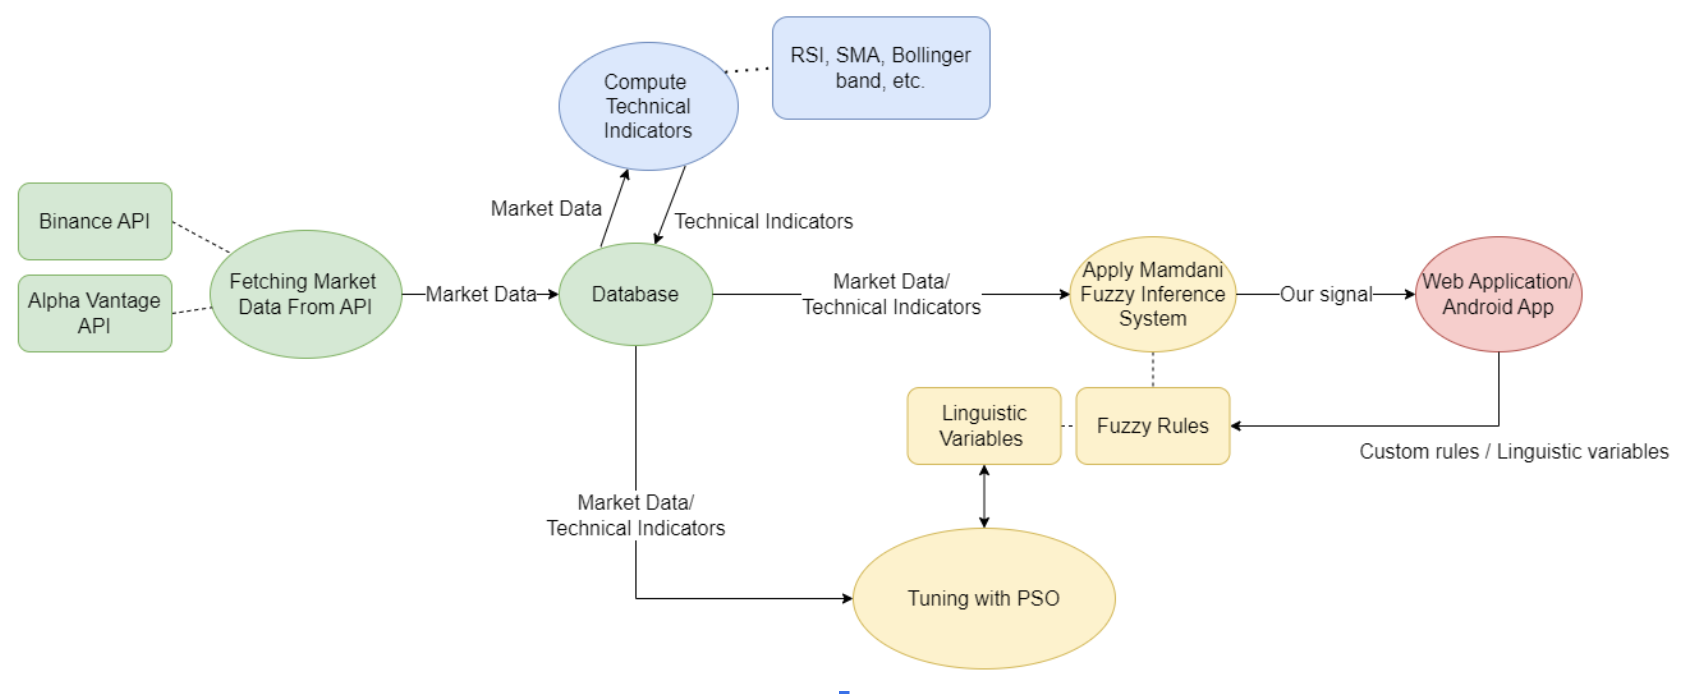
\includegraphics[scale=0.3]{images/overview.png}
    \caption{แผนภาพกระแสข้อมูล}
    \label{fig:11}
\end{figure}

\section{เว็บแอปพลิเคชัน}
เว็บแอปพลิเคชันสามารถรองรับการทำงานของผู้ใช้งานทั้งบนคอมพิวเตอร์และโทรศัพท์มือถือ \\
จุดประสงค์ของเว็บแอปพลิเคชันคือเป็นส่วนติดต่อให้กับผู้ใช้งานที่ต้องการเข้ามาใช้ระบบของเราโดยมีส่วนที่ต้องรองรับหลักดังนี้
\begin{itemize}
    \item ผู้ใช้งานสามารถดูกราฟ OHLC ของสินทรัพย์ในแต่ละ Interval
    \item ผู้ใช้งานสามารถเพิ่มเครื่องมือตัวชี้วัดเบื้องต้นที่ต้องการอย่างเช่น RSI, MACD, และตัวอื่นๆที่ระบบของเรามีให้
    \item ผู้ใช้งานสามารถสร้าง Preset และปรับแต่งระบบ Fuzzy logic (ปรับกฏ และตัวแปรทางภาษา)
    \item ผู้ใช้งานสามารถดูผลลัพธ์ที่ได้จาก Preset ระบบ Fuzzy logic
    \item ผู้ใช้งานสามารถทำการทดสอบกลยุทธ์ย้อนหลัง Backtesting บน Preset Fuzzy logic และดูผลลัพธ์การทดสอบ
    \item ผู้ใช้งานสามารถทำปรับจูนตัวแปรทางภาษาของ Preset Fuzzy logic ด้วย PSO และดูผลลัพธ์การปรับจูน
\end{itemize}
ทำการออกแบบ UI/UX ของเว็บแอปพลิเคชัน Figma
โดยในการพัฒนาเว็บแอปพลิเคชันส่วนหลักใช้ UI Framework อย่าง SvelteKit และภาษา TypeScript

\subsection{เว็บเซิร์ฟเวอร์}
ก่อนจะเรียกใช้ APIs ต่างๆของเรานั้นผู้ใช้ต้องทำการสร้างบัญชีเอาไว้ก่อนเพื่อให้สามารถเก็บค่าการปรับแต่ง Fuzzy logic ที่ผู้ใช้แต่ละคนทำไว้ได้ แล้ว Endpoints
แต่ละอันนั้นก็ต้องส่ง Bearer Token ยืนยันตัวผู้ใช้มาด้วยโดยเราจะมี Endpoints ดังต่อไปนี้
\begin{enumerate}
    \overfullrule=0pt
    \item \texttt{GET {\footnotesize /api/ohlc?symbol=[supported\_symbols]\&interval=[1d|4h|1h]}} \\ให้ข้อมูล OHLC ของสินทรัพย์ตาม supported\_symbols และ interval
    % \item \texttt{POST {\footnotesize /api/users/[]}} \\ทำอะไรวะ
    \item \texttt{GET {\footnotesize /api/indicators/macd?symbol=[supported\_symbols]\&interval=[1d|4h|1h]}} \\ให้ข้อมูลตัวชี้วัด MACD ของสินทรัพย์ตาม supported\_symbols และ interval
    \item \texttt{GET {\footnotesize /api/indicators/macd/transformed?symbol=[supported\_symbols]\&interval=[1d|4h|1h]}} \\ให้ข้อมูลตัวชี้วัด MACD Transformed ของสินทรัพย์ตาม supported\_symbols และ interval
    \item \texttt{GET {\footnotesize /api/indicators/rsi?symbol=[supported\_symbols]\&interval=[1d|4h|1h]}} \\ให้ข้อมูลตัวชี้วัด RSI ของสินทรัพย์ตาม supported\_symbols และ interval
    \item \texttt{GET {\footnotesize /api/indicators/bb?symbol=[supported\_symbols]\&interval=[1d|4h|1h]}} \\ให้ข้อมูลตัวชี้วัด BB ของสินทรัพย์ตาม supported\_symbols และ interval
    \item \texttt{GET {\footnotesize /api/indicators/adx?symbol=[supported\_symbols]\&interval=[1d|4h|1h]}} \\ให้ข้อมูลตัวชี้วัด ADX ของสินทรัพย์ตาม supported\_symbols และ interval
    \item \texttt{GET {\footnotesize /api/indicators/obv?symbol=[supported\_symbols]\&interval=[1d|4h|1h]}} \\ให้ข้อมูลตัวชี้วัด OBV ของสินทรัพย์ตาม supported\_symbols และ interval
    \item \texttt{GET {\footnotesize /api/indicators/aroon?symbol=[supported\_symbols]\&interval=[1d|4h|1h]}} \\ให้ข้อมูลตัวชี้วัด AROON ของสินทรัพย์ตาม supported\_symbols และ interval
    \item \texttt{GET {\footnotesize /api/indicators/accumdist?symbol=[supported\_symbols]\&interval=[1d|4h|1h]}} \\ให้ข้อมูลตัวชี้วัด ACCUM DIST ของสินทรัพย์ตาม supported\_symbols และ interval
    \item \texttt{GET {\footnotesize /api/indicators/stoch?symbol=[supported\_symbols]\&interval=[1d|4h|1h]}} \\ให้ข้อมูลตัวชี้วัด STOCH ของสินทรัพย์ตาม supported\_symbols และ interval
    \item \texttt{GET {\footnotesize /api/fuzzy?symbol=[supperted\_symbols]\&interval=[1d|4h|1h]\&preset=[preset]}} \\ให้ข้อมูลตัวชี้วัด fuzzy preset ของสินทรัพย์ supported\_symbols และ interval
    \item \texttt{GET {\footnotesize /api/settings?preset=[[preset]]}} \\ให้ข้อมูลการตั้งค่าของ fuzzy preset
    \item \texttt{PUT {\footnotesize /api/settings/linguisticvars?preset=[preset]}} \\อัพเดทค่าตัวแปรทางภาษาของ fuzzy preset
    \item \texttt{DELETE {\footnotesize /api/settings/linguisticvars/[name]?preset=[preset]}} \\ลบตัวแปรทางภาษาตามชื่อ name ใน fuzzy preset
    \item \texttt{POST {\footnotesize /api/settings/fuzzyrules?preset=[preset]}} \\เพิ่มกฏฟัซซีใน fuzzy preset
    \item \texttt{DELETE {\footnotesize /api/settings/fuzzyrules/[id]}} \\ลบกฏฟัซซีตาม id ใน fuzzy preset
    \item \texttt{GET {\footnotesize /api/settings/presets}} \\ให้ข้อมูลรายชื่อ fuzzy preset ที่มีอยู่
    \item \texttt{POST {\footnotesize /api/settings/presets/[preset]}} \\สร้าง fuzzy preset ด้วยชื่อ preset
    \item \texttt{DELETE {\footnotesize /api/settings/presets/[preset]}} \\ลบ fuzzy preset ที่ชื่อ preset
    \item \texttt{PUT {\footnotesize /api/settings/users}} \\อัพเดทข้อมูลการตั้งค่าตัวชี้วัดทางเทคนิคของ user
    \item \texttt{GET {\footnotesize /api/settings/users}} \\ให้ข้อมูลการตั้งค่าตัวชี้วัดทางเทคนิคของ user
    \item \texttt{POST {\footnotesize /api/backtesting/run?preset=[preset]}} \\ทดสอบกลยุทธ์ fuzzy preset ย้อนหลัง
    \item \texttt{GET {\footnotesize /api/backtesting/running}} \\ให้ข้อมูลจำนวนการทดสอบกลยุทธ์ที่กำลังดำเนินการ
    \item \texttt{GET {\footnotesize /api/backtesting}} \\ให้ข้อมูลผลการทดสอบกลยุทธ์ทั้งหมดที่มี
    \item \texttt{GET {\footnotesize /api/backtesting/[id]}} \\ให้ข้อมูลผลการทดสอบกลยุทธ์ตาม id
    \item \texttt{DELETE {\footnotesize /api/backtesting/[id]}} \\ลบข้อมูลผลการทดสอบกลยุทธ์ตาม id
    % \item \texttt{DELETE {\footnotesize /api/backtesting}} \\ทำอะไรวะ
    \item \texttt{POST {\footnotesize /api/pso/run/[preset]?symbol=[supported\_symbols]\&interval=[1d|4h|1h]\&runtype=[normal|crossvalid]}} \\ปรับจูนตัวแปรทางภาษาบน fuzzy preset ด้วย PSO
    \item \texttt{GET {\footnotesize /api/pso}} \\ให้ข้อมูลผลการปรับจูนด้วย PSO
    \item \texttt{DELETE {\footnotesize /api/pso/[id]}} \\ลบข้อมูลผลการปรับจูนด้วย PSO
    \item \texttt{GET {\footnotesize /api/pso/running}} \\ให้ข้อมูลจำนวนการปรับจูนด้วย PSO ที่กำลังดำเนินการ
    \item \texttt{GET {\footnotesize /api/user}} \\ให้ข้อมูลความถูกต้องของ user
\end{enumerate}
โดยที่ supported\_symbols มีดังนี้
ิ\begin{itemize}
    \item ETH/USDT
    \item BTC/USDT
    \item BNB/USDT
    \item AAPL/USD
    \item IBM/USD
    \item JPM/USD
    \item MSFT/USD
    \item NKE/USD
    \item TSLA/USD
\end{itemize}

\subsection{การใช้งานเว็บแอปพลิเคชัน}
หลังจาก Login เข้าเว็บแล้ว เว็บแอปพลิเคชันจะแบ่งการทำงานเป็น 4 หน้าหลักดังนี้
\begin{itemize}
    \item หน้า Chart สำหรับแสดงผลกราฟ OHLC ของตลาดสินทรัพย์, ตัวชี้วัดทางเทคนิค
    \item หน้า Settings สำหรับการสร้าง/แก้ไข/ลบ Preset ของระบบ Fuzzy logic
    \item หน้า Backtests สำหรับทำการทดสอบกลยุทธ์ย้อนหลัง และดูผลลัพธ์การทดสอบ
    \item หน้า PSO สำหรับการปรับจูนตัวแปรทางภาษาด้วย PSO และดูผลลัพธ์การปรับจูน
\end{itemize}

\subsubsection{การใช้งานหน้า Chart}
.....

\subsubsection{การใช้งานหน้า Settings}
.....

\subsubsection{การใช้งานหน้า Backtests}
.....

\subsubsection{การใช้งานหน้า PSO}
.....
\def\checkmark{\tikz\fill[scale=0.4](0,.35) -- (.25,0) -- (1,.7) -- (.25,.15) -- cycle;}

\chapter{\ifproject%
      \ifenglish Experimentation and Results\else การทดลองและผลลัพธ์\fi
  \else%
      \ifenglish System Evaluation\else การประเมินระบบ\fi
  \fi}

\section{คำอธิบายการทดลอง}
ในการทดลองนี้เราจะใช้ระบบที่เราสร้างขึ้นมาในการทำการทดสอบโดยใช้เงินตั้งต้น 3,000 USD และทดสอบบนตลาด Crypto Currency (BTC, ETH, BNB) และตลาดหุ้น NASDAQ (AAPL, IBM, JPM, MSFT, NKE, TSLA) ซึ่งเงินตั้งต้นจะถูกแบ่งให้เท่าๆ กันจาก 3,000 USD สำหรับแต่ละเหรียญหรือหุ้นในทั้ง 2 ตลาด โดยวิธีการเข้าซื้อจะมีดังนี้

\begin{table}[ht]
    \centering
    \resizebox{\columnwidth}{!}{%
        \begin{tabular}{lccccc}
            \textbf{ส่วนเสริม}                                                                                                         &
            \multicolumn{1}{l}{\textbf{Classical}}                                                                                   &
            \multicolumn{1}{l}{\textbf{Fuzzy}}                                                                                       &
            \multicolumn{1}{l}{\textbf{Fuzzy C}}                                                                                     &
            \multicolumn{1}{l}{\textbf{Fuzzy PSO}}                                                                                   &
            \multicolumn{1}{l}{\textbf{Fuzzy PSO}}                                                                                                                                           \\
            ใช้ Fuzzy Logic ในการทำอินดิเคเตอร์ขึ้นมา                                                                                       &   & \checkmark &            & \checkmark & \checkmark \\
            \begin{tabular}[c]{@{}l@{}}การจัดการเงินทุนโดยใช้ค่าของอินดิเคเตอร์จาก  Fuzzy Logic\\ (Liquidation F)\end{tabular}               &   &            & \checkmark &            & \checkmark \\
            \begin{tabular}[c]{@{}l@{}}การใช้ Particle Swarm Optimization (PSO) ในการปรับค่าของตัว\\ แปรทางภาษาของอินดิเคเตอร์\end{tabular} &   &            &            & \checkmark & \checkmark
        \end{tabular}%
    }
    \caption{ตัวชี้วัดที่นำมาใช้ในการเข้าซื้อ}
    \label{tab:indicators}
\end{table}
โดยสำหรับวิธี Classical นั้นเราจะใช้ค่าของอินดิเคเตอร์แต่ละตัวตรงๆ มาใช้ตัดสินใจเข้าซื้อ และการใช้ PSO ในการปรับค่าของตัวแปรทางภาษาจะมีพารามิเตอร์ตังนี้
\begin{itemize}
    \item {จำนวนกลุ่ม (Swarm Size) ที่ใช้ในการฝึกสอน จะมี 3 รูปแบบ คือ 5, 10, 15}
    \item {จำนวนสมาชิกในแต่ละกลุ่ม (Number of Particles) จะเป็น 10}
    \item {เงื่อนไขในการจบการทำงาน คือเมื่อถึงรอบที่ 10}
\end{itemize}
โดยเราจะฝึกสอนโดยใช้ข้อมูลตั้งแต่จุดเริ่มต้นของข้อมูลตลาดแต่ละตลาด ถึงจุดเริ่มต้นของช่วง validation ซึ่งจะเป็น 6 เดือนก่อนหน้าวันที่ 1 ตุลาคม 2023 และเราก็จะใช้กรอบเวลาของข้อมูลเป็นสี่ชั่วโมง (4h) ซึ่งสามารถดูผลของการใช่ PSO ได้ในภาคผนวก จากนั้นเราก็จะเลือกตัวที่ให้ผลลัพธ์ที่ดีที่สุดแล้วไปใช้ในการทดสอบต่อไป ในส่วนของด้านล่างนี้เป็นเงื่อนไขอื่นๆ สำหรับการทดสอบ
\begin{itemize}
    \item {มีการเข้าซื้อขั้นต่ำอยู่ที่ 30 USD}
    \item {สำหรับการเข้าซื้อแบบที่ไม่ได้การจัดการเงินทุนจะเข้าซื้อที่ 5\% ของเงินที่มีอยู่ขณะนั้น}
    \item {สำหรับตลาด Crypto Curreny เมื่อกำไรของการเข้าซื้อนั้น ≥ 20\% (take profit) หรือเมื่อขาดทุน ≥ 10\% (stop loss) เราจะขายออก}
    \item {สำหรับตลาดหุ้น NASDAQ เมื่อกำไรของการเข้าซื้อนั้น ≥ 10\% (take profit) หรือเมื่อขาดทุน ≥ 5\% (stop loss) เราจะขายออก}
\end{itemize}
นอกจากนี้เราจะมีวิธี Buy \& Hold ซึ่งเป็นวิธีการซื้อสินทรัพย์ไว้ด้วยจำนวนเงินทั้งหมด ตั้งแต่วันแรกที่ทดสอบไว้แล้วถือไว้โดยไม่ขายออกเป็นตัวไว้เปรียบเทียบ การทดสอบจะเริ่มตั้งแต่วันที่ 1 ตุลาคม 2023 ถึง 8 มีนาคม 2024 เป็นเวลาประมาณ 5 เดือน โดยใช้กรอบเวลาเป็นทั้ง 1 ชั่วโมง (1h) และ 1 วัน (1d) เพื่อสังเกตุความแตกต่างของผลลัพธ์ที่ได้จากการใช้กรอบเวลาที่ต่างกัน 

และเราก็จะมีการทดลองกับตลาดที่มีทิศทางไม่แน่นอน และตลาดขาลงด้วยเช่นกัน โดยเราจะทดสอบบนตลาด Crypto Currency โดยใช้เหรียญ ETH อย่างเดียว เพื่อให้เรามารถเลือกช่วงที่แนวโน้มของตลาดเปลี่ยนไปได้ง่าย โดยจะใช้การทดสอบแบบเดียวกับการทดสอบที่กล่าวมาก่อนหน้านี้ โดยมีเงินเริ่มที่ 3,000 USD มาใช้กับ ETH และทดสอบในช่วงเวลาที่ต่างกัน โดยที่ช่วงเวลาของแต่ละการทดสอบจะเป็น
\begin{itemize}
    \item ช่วงที่ตลาดมีทิศทางไม่แน่นอนจะเริ่มที่ 15 พฤษจิกายน 2021 ถึง 16 เมษายน 2022 เป็นเวลาประมาณ 6 เดือน
    \item ช่วงที่ตลาดเป็นขาลงจะเริ่มที่ 16 กรกฎาคม 2022 ถึง 5 มกราคม 2023 เป็นเวลาประมาณ 6 เดือน
\end{itemize}
เราจะใช้ตัวชี้วัดสองตัวในการทำการทดสอบ ได้แก่ AROON-MACD และ RSI-BB ที่เราสร้างขึ้นมา โดยจะมีคำอธิบายของตัวชี้วัดแต่ละตัวดังนี้

\subsection{ตัวชี้วัด AROON-MACD}
\begin{table}[ht]
    \centering
    \begin{tabular}{llllll}
        \hline
           & MACD                          & AROONUP & AROONDOWN & Long & Short \\ \hline
        If & $(>65 \& <85) | (>35 | < 65)$ & $>80$   &           & $1$  &       \\ \hline
        If & $(>15 \& <35) | (>35 | < 65)$ &         & $>80$     &      & $1$   \\ \hline
    \end{tabular}
    \caption{วิธีการเข้าซื้อแบบ Classical ของตัวชี้วัด AROON-MACD}
\end{table}

สำหรับตัวชี้วัดตัวนี้จะมีตัวแปรทางภาษาตามรูปที่ \ref{fig:aroon-macd-lin} ในภาคผนวก และมี Fuzzy Rules ดังรูปที่ \ref{fig:aroon-macd-rules}
\begin{figure}[!ht]
    \centering
    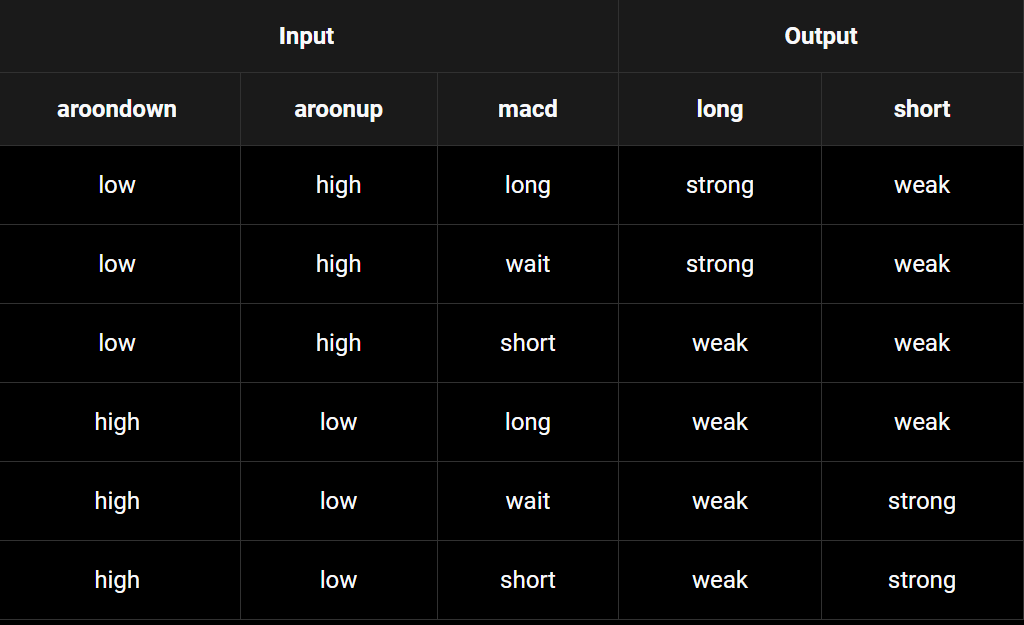
\includegraphics[width=\textwidth]{images/aroon-macd-rules.png}
    \caption{Fuzzy Rules ของตัวชี้วัด AROON-MACD}
    \label{fig:aroon-macd-rules}
\end{figure}
โดยสำหรับตัวชี้วัดนี้จะเป็นตัวชี้วัดแบบ Trend Following ซึ่งคือการที่เราพยายามซื้อขายสินทรัพย์ตามแนวโน้มของตลาด ถ้าตลาดกำลังอยู่ในขาขึ้นก็จะมีการทำการเข้าซื้อแบบ long และถ้าตลาดกำลังอยู่ในขาลงก็จะมีการทำการเข้าซื้อแบบ short โดย MACD จะเป็นตัวที่บอกเราว่าควรเข้าซื้อ ณ เวลาไหน และ AROON จะเป็นตัวบอกเราว่าตลาดกำลังอยู่ในขาขึ้นหรือขาลง โดยเราจะเข้าซื้อเมื่อค่าของอินดิเคเตอร์มีค่าเกิน 30

\subsection{ตัวชี้วัด RSI-BB}
\begin{table}[ht]
    \centering
    \begin{tabular}{lllll}
        \hline
           & RSI   & BB     & Long & Short \\ \hline
        If & $<30$ & $<-80$ & $1$  &       \\ \hline
        If & $>70$ & $>80$  &      & $1$   \\ \hline
    \end{tabular}
    \caption{วิธีการเข้าซื้อแบบ Classical ของตัวชี้วัด RSI-BB}
\end{table}

สำหรับตัวชี้วัดตัวนี้จะมีตัวแปรทางภาษาตามรูปที่ \ref{fig:rsi-bb-lin} ในภาคผนวก และมี Fuzzy Rules ดังรูปที่ \ref{fig:rsi-bb-rules}
\begin{figure}[!ht]
    \centering
    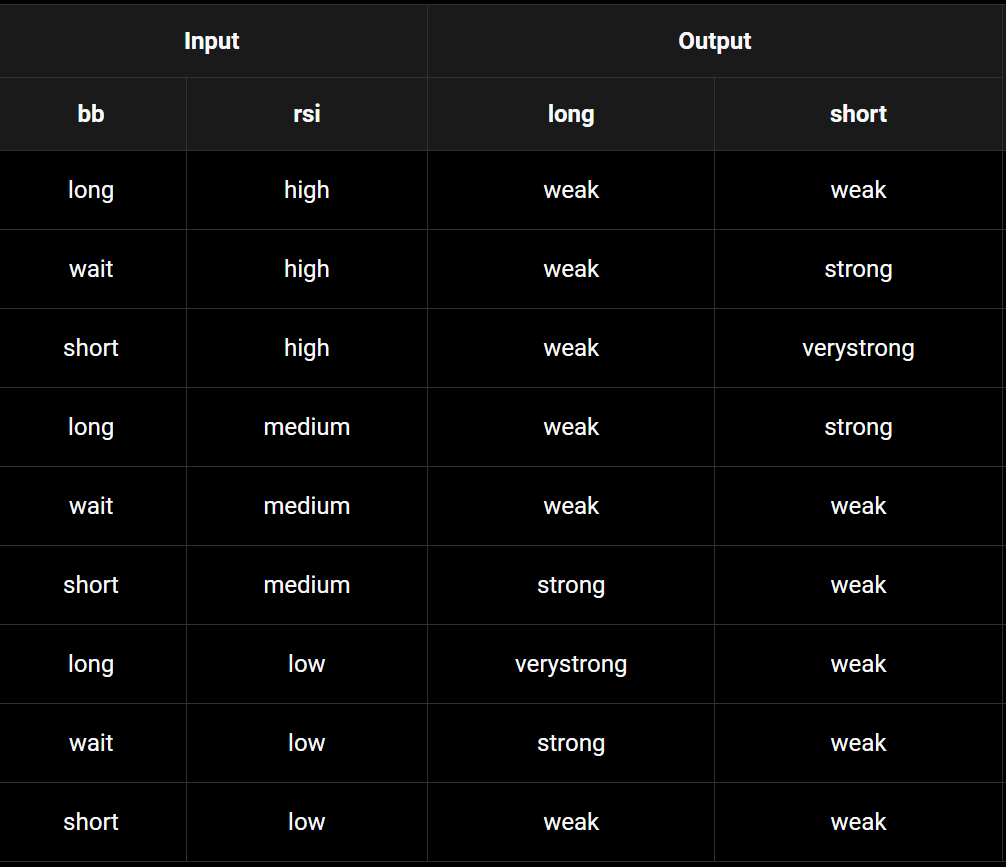
\includegraphics[width=0.8\textwidth]{images/rsi-bb-rules.png}
    \caption{Fuzzy Rules ของตัวชี้วัด RSI-BB}
    \label{fig:rsi-bb-rules}
\end{figure}
โดยสำหรับตัวชี้วัดนี้จะเป็นตัวชี้วัดแบบ Mean Reversion ซึ่งคือการที่เราคาดว่าราคาของสินทรัพย์จะมีแนวโน้มที่จะกลับมาสู่ราคาเฉลี่ย โดย Bollinger Band (BB) จะเป็นตัวบอกว่าราคาของสินทรัพย์นั้นสูงหรือต่ำกว่าค่าเฉลี่ยเกินไปหรือไม่ และ RSI จะเป็นตัวที่บอกเราว่าควรเข้าซื้อ ณ ตอนไหน ถ้าราคาของสินทรัพย์นั้นต่ำกว่าค่าเฉลี่ย และ RSI บอกว่าสินทรัพย์นั้นมีการขายอย่างมาก เราก็จะเข้าซื้อแบบ long และถ้าราคาของสินทรัพย์นั้นสูงกว่าค่าเฉลี่ย และ RSI บอกว่าสินทรัพย์นั้นมีการซื้ออย่างมาก เราก็จะเช้าซื้อแบบ short โดย เราจะเข้าซื้อเมื่อค่าของอินดิเคเตอร์นี้มีค่าเกิน 25

\section{ผลการทดลอง}
\begin{table}[!htb]
    \centering
    \begin{tabular}{crrrrr}
        \hline
        \textbf{Symbol} & \textbf{Classical} & \textbf{Fuzzy} & \textbf{Fuzzy C} & \textbf{Fuzzy PSO} & \textbf{Fuzzy PSO C} \\ \hline
        BTC             & 680.48             & 654.28         & 1035.67          & 1383.01            & \textbf{1450.66}     \\ \hline
        ETH             & 440.45             & 509.39         & 509.16           & 294.08             & \textbf{1264.20}     \\ \hline
        BNB             & 448.98             & 496.05         & 736.79           & 554.83             & \textbf{926.30}      \\ \hline
        TOTAL           & 1569.91            & 1659.72        & 2281.62          & 2231.92            & \textbf{3641.15}     \\ \hline
    \end{tabular}
    \caption{ผลกำไรขาดทุนของการทดสอบตัวชี้วัด AROON-MACD ในตลาด Crypto Currency (หน่วยเป็น USD) ด้วยกรอบเวลา 1 ชั่วโมง (1h)}
    \label{tab:aroon-macd-crypto}
\end{table}

\begin{table}[!htb]
    \centering
    \begin{tabular}{crrrrr}
        \hline
        \textbf{Symbol} & \textbf{Classical} & \textbf{Fuzzy} & \textbf{Fuzzy C} & \textbf{Fuzzy PSO} & \textbf{Fuzzy PSO C} \\ \hline
        AAPL            & \textbf{4.41}      & 0.37           & -0.01            & -18.55             & -23.70               \\ \hline
        IBM             & \textbf{81.12}     & 62.58          & 28.71            & 74.48              & 75.30                \\ \hline
        JPM             & 13.59              & \textbf{20.73} & 20.72            & 7.41               & -10.78               \\ \hline
        MSFT            & \textbf{90.80}     & 64.01          & 64.80            & 59.54              & 6.60                 \\ \hline
        NKE             & \textbf{45.31}     & 23.76          & 23.68            & 23.71              & -27.81               \\ \hline
        TSLA            & \textbf{171.23}    & 59.16          & 56.97            & 6.73               & -3.14                \\ \hline
        TOTAL           & \textbf{406.46}    & 230.62         & 194.87           & 153.30             & 16.47                \\ \hline
    \end{tabular}
    \caption{ผลกำไรขาดทุนของการทดสอบตัวชี้วัด AROON-MACD ในตลาดหุ้น NASDAQ (หน่วยเป็น USD) ด้วยกรอบเวลา 1 ชั่วโมง (1h)}
    \label{tab:aroon-macd-stocks}
\end{table}
\FloatBarrier
\pagebreak

\begin{table}[!htb]
    \centering
    \begin{tabular}{crrrrr}
        \hline
        \textbf{Symbol} & \textbf{Classical} & \textbf{Fuzzy} & \textbf{Fuzzy C} & \textbf{Fuzzy PSO} & \textbf{Fuzzy PSO C} \\ \hline
        BTC             & -110.64            & -105.57        & -96.40           & 1381.81            & \textbf{1466.41}     \\ \hline
        ETH             & -84.48             & -24.46         & -49.72           & \textbf{1261.53}   & -49.72               \\ \hline
        BNB             & -109.26            & 28.17          & 20.36            & 28.17              & \textbf{1044.98}     \\ \hline
        TOTAL           & -304.38            & -101.87        & -125.76          & \textbf{2671.50}   & 2461.67              \\ \hline
    \end{tabular}
    \caption{ผลกำไรขาดทุนของการทดสอบตัวชี้วัด RSI-BB ในตลาด Crypto Currency (หน่วยเป็น USD) ด้วยกรอบเวลา 1 ชั่วโมง (1h)}
    \label{tab:rsi-bb-crypto}
\end{table}

\begin{table}[!htb]
    \centering
    \begin{tabular}{crrrrr}
        \hline
        \textbf{Symbol} & \textbf{Classical} & \textbf{Fuzzy} & \textbf{Fuzzy C} & \textbf{Fuzzy PSO} & \textbf{Fuzzy PSO C} \\ \hline
        AAPL            & \textbf{17.09}     & -20.55         & -20.55           & -21.33             & -3.53                \\ \hline
        IBM             & -50.07             & 69.16          & 53.64            & \textbf{172.27}    & 17.32                \\ \hline
        JPM             & -57.70             & \textbf{24.27} & 20.96            & -112.47            & -109.25              \\ \hline
        MSFT            & -25.98             & 37.86          & 41.21            & \textbf{89.50}     & -15.32               \\ \hline
        NKE             & -7.20              & -45.88         & -45.88           & -45.88             & -22.72               \\ \hline
        TSLA            & -14.12             & \textbf{2.70}  & \textbf{2.70}    & -64.64             &
        \textbf{2.70}                                                                                                        \\ \hline
        TOTAL           & -137.99            & \textbf{67.56} & 52.08            & 17.45              & -130.80              \\ \hline
    \end{tabular}
    \caption{ผลกำไรขาดทุนของการทดสอบตัวชี้วัด RSI-BB ในตลาดหุ้น NASDAQ (หน่วยเป็น USD) ด้วยกรอบเวลา 1 ชั่วโมง (1h)}
    \label{tab:rsi-bb-stocks}
\end{table}

\begin{figure}[!htb]
    \centering
    \subfigure[1h]{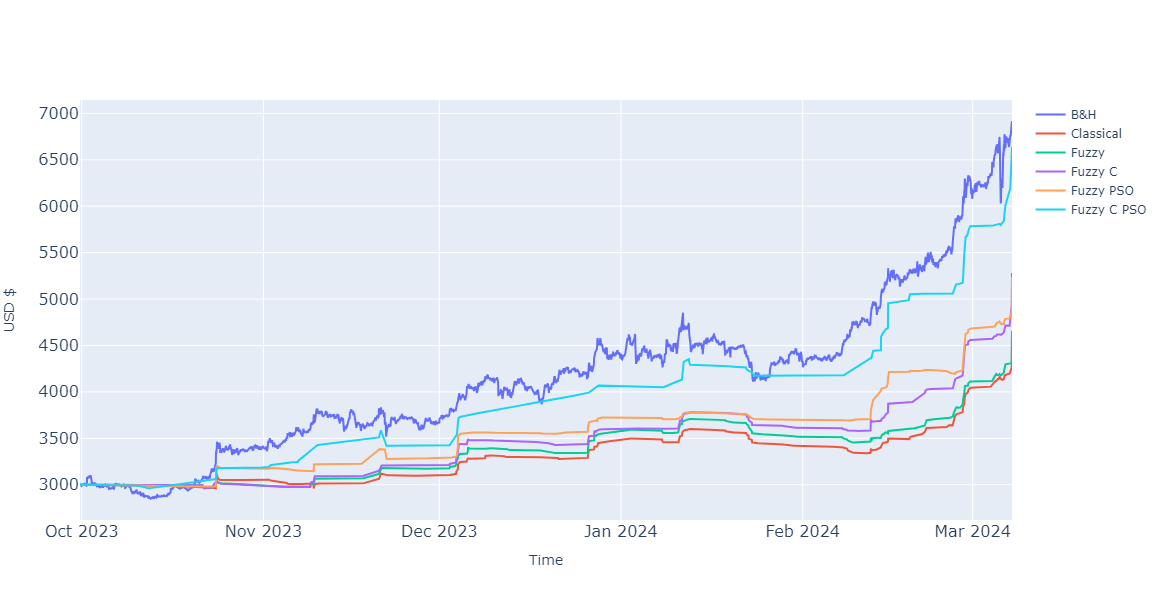
\includegraphics[width=0.95\textwidth]{images/aroon-macd/crypto-result.png}
        \label{fig:aroon-macd-crypto}}
    \subfigure[1d]{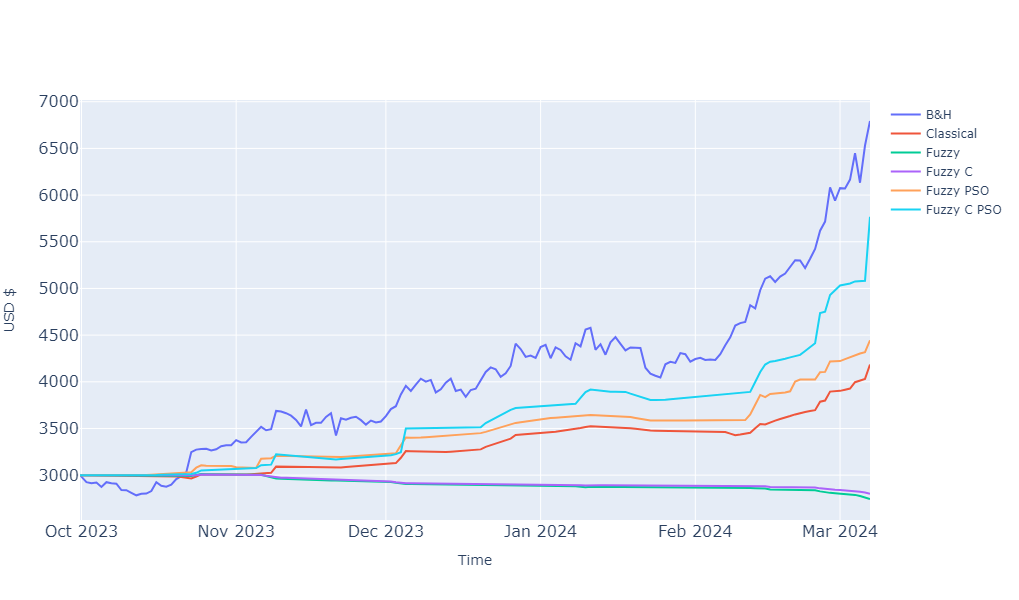
\includegraphics[width=0.95\textwidth]{images/aroon-macd/crypto-result-1d.png}}
    \caption{ความเปลี่ยนของเงินลงทุนของตัวชี้วัด AROON-MACD ในตลาด Crypto Currency ในแต่ละกรอบเวลา}
    \label{fig:aroon-macd-crypto-all}
\end{figure}

\begin{figure}[!htb]
    \centering
    \subfigure[1h]{
        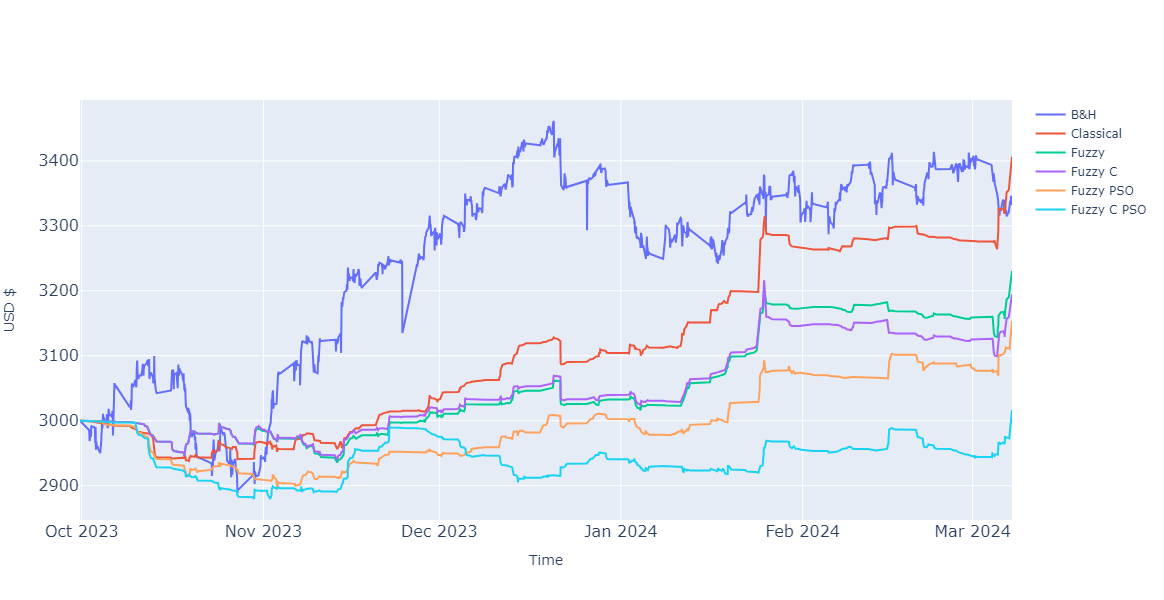
\includegraphics[width=0.95\textwidth]{images/aroon-macd/stock-result.png}
        \label{fig:aroon-macd-stock}
    }
    \subfigure[1d]{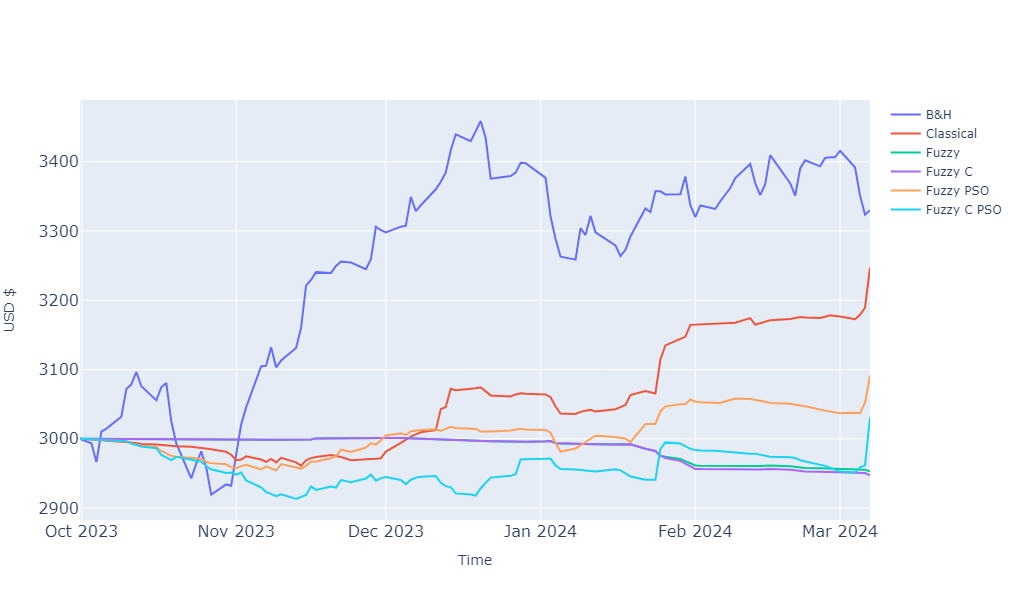
\includegraphics[width=0.95\textwidth]{images/aroon-macd/stock-result-1d.png}}
    \caption{ความเปลี่ยนของเงินลงทุนของตัวชี้วัด AROON-MACD ในตลาดหุ้น NASDAQ ในแต่ละกรอบเวลา}
    \label{fig:aroon-macd-stock-all}
\end{figure}

\begin{figure}[!htb]
    \centering
    \subfigure[1h]{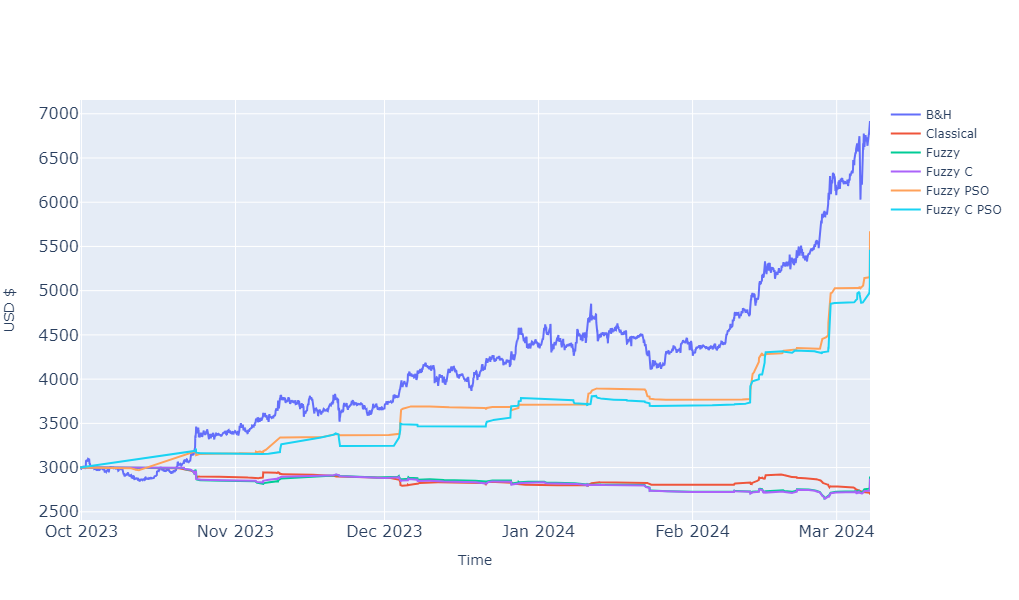
\includegraphics[width=0.95\textwidth]{images/rsi-bb/crypto-result.png}
        \label{fig:rsi-bb-crypto}
    }
    \subfigure[1d]{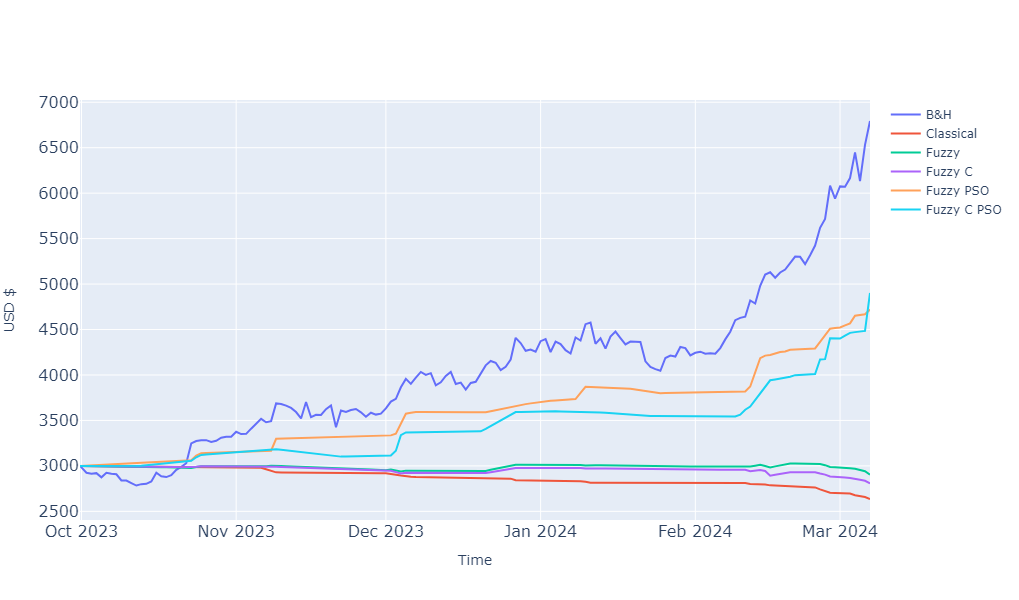
\includegraphics[width=0.95\textwidth]{images/rsi-bb/crypto-result-1d.png}}
    \caption{ความเปลี่ยนของเงินลงทุนของตัวชี้วัด RSI-BB ในตลาด Crypto Currency ในแต่ละกรอบเวลา}
    \label{fig:rsi-bb-crypto-all}
\end{figure}

\begin{figure}[!htb]
    \centering
    \subfigure[1h]{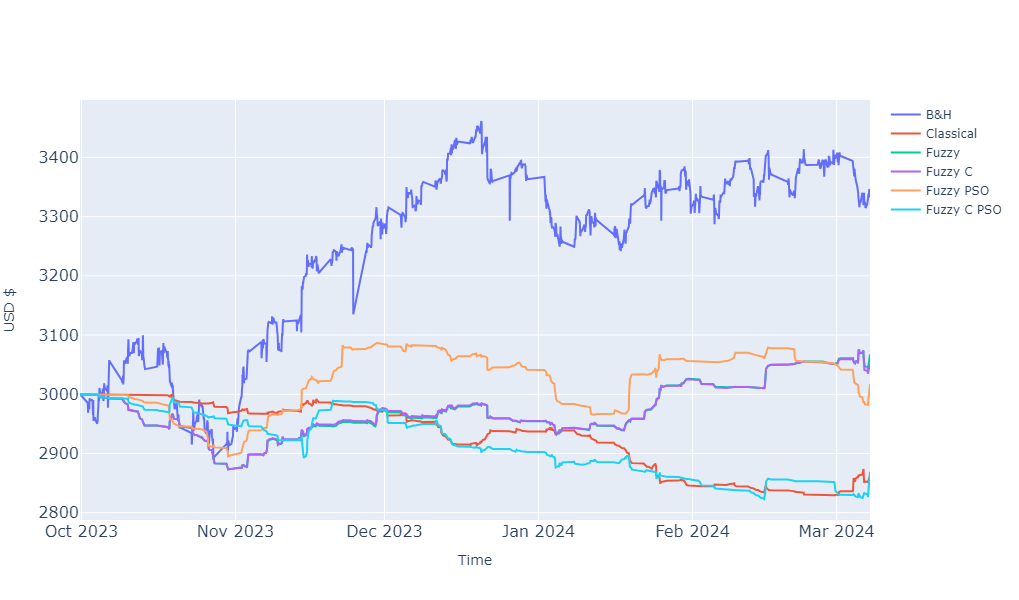
\includegraphics[width=0.95\textwidth]{images/rsi-bb/stock-result.png}
        \label{fig:rsi-bb-stock}
    }
    \subfigure[1d]{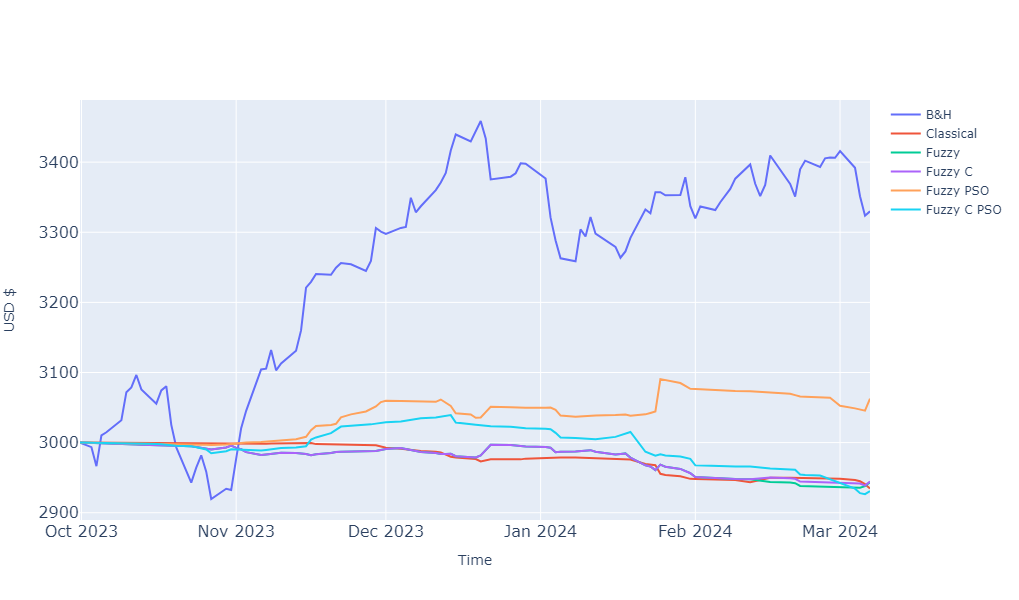
\includegraphics[width=0.95\textwidth]{images/rsi-bb/stock-result-1d.png}}
    \caption{ความเปลี่ยนของเงินลงทุนของตัวชี้วัด RSI-BB ในตลาดหุ้น NASDAQ ในแต่ละกรอบเวลา}
    \label{fig:rsi-bb-stock-all}
\end{figure}

\begin{figure}[!htb]
    \centering
    \subfigure[sideway]{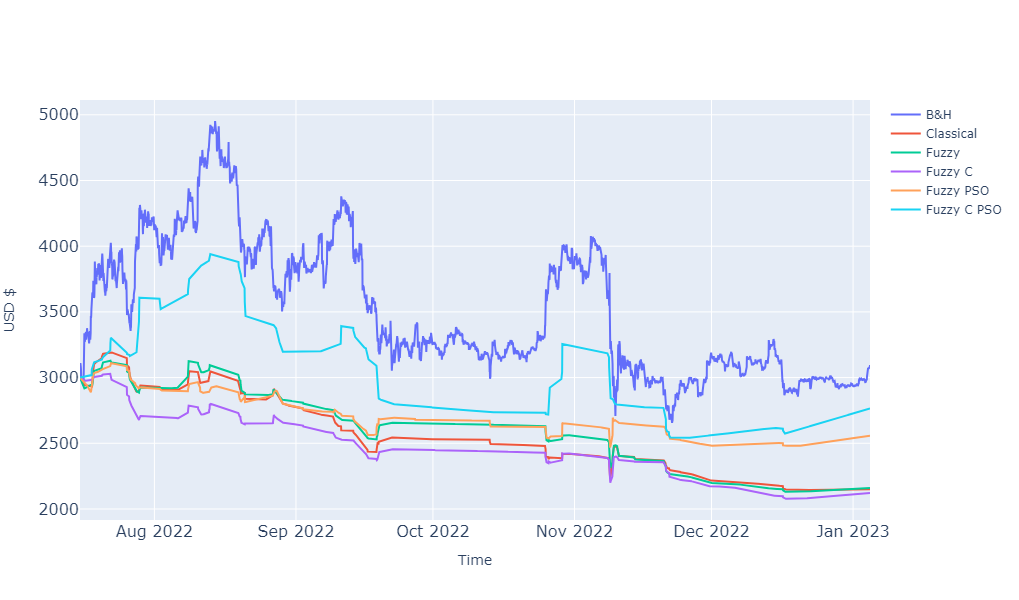
\includegraphics[width=0.95\textwidth]{images/aroon-macd/sideway.png}\label{fig:aroon-macd-side}}
    \subfigure[downtrend]{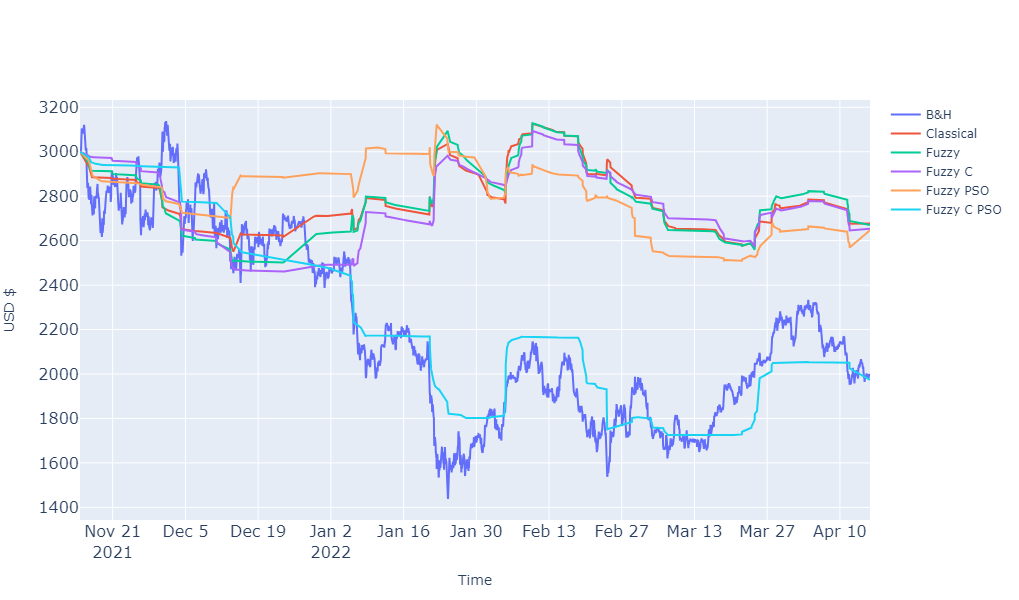
\includegraphics[width=0.95\textwidth]{images/aroon-macd/bear.png}\label{fig:aroon-macd-down}}
    \caption{ความเปลี่ยนของเงินลงทุนของตัวชี้วัด AROON-MACD ในตลาด Crypto Currency (ETH) ในแนวโน้มตลาดแบบทิศทางไม่แน่นอน (sideway) และแบบขาลง (downtrend)}
\end{figure}

\begin{figure}[!htb]
    \centering
    \subfigure[sideway]{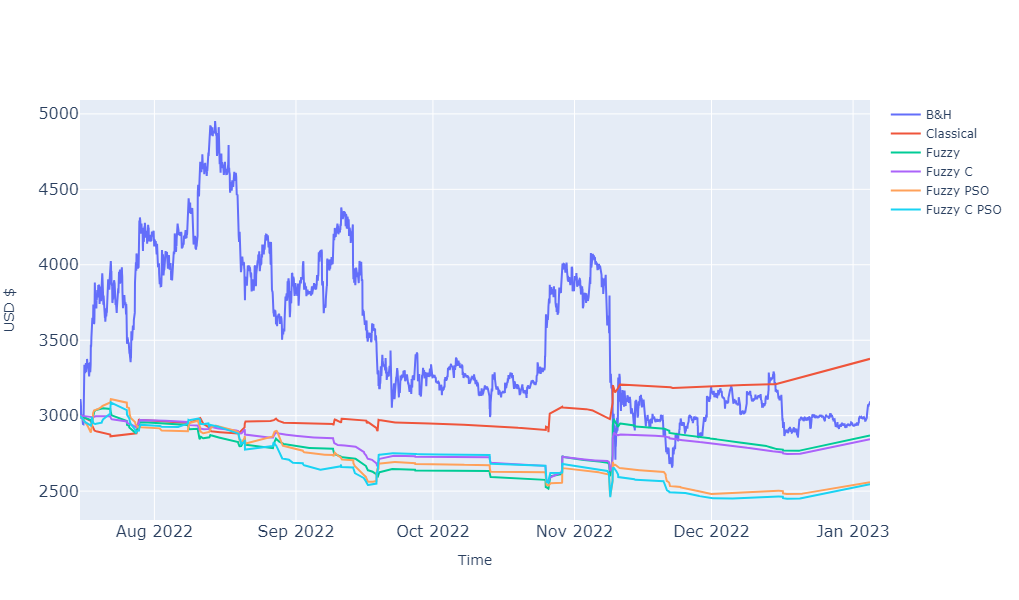
\includegraphics[width=0.95\textwidth]{images/rsi-bb/sideway.png}\label{fig:rsi-bb-side}}
    \subfigure[downtrend]{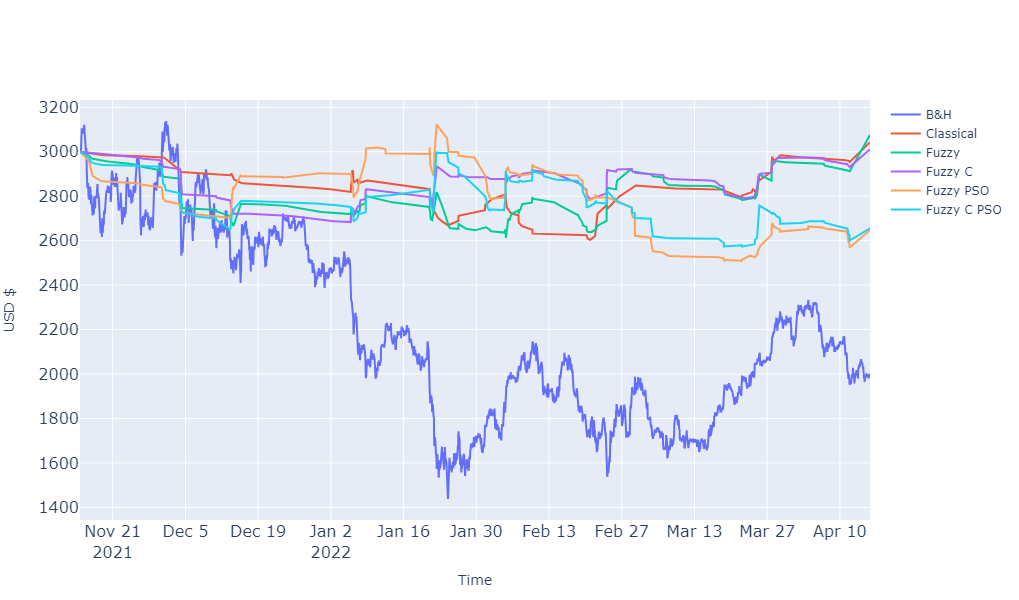
\includegraphics[width=0.95\textwidth]{images/rsi-bb/bear.png} \label{fig:rsi-bb-down}}
    \caption{ความเปลี่ยนของเงินลงทุนของตัวชี้วัด RSI-BB ในตลาด Crypto Currency (ETH) ในแนวโน้มตลาดแบบทิศทางไม่แน่นอน (sideway) และแบบขาลง (downtrend)}
\end{figure}
\FloatBarrier

\section{ผลการวิเคราะห์}
\subsection{ตัวชี้วัด AROON-MACD}
จากตารางที่ \ref{tab:aroon-macd-crypto} และรูปที่ \ref{fig:aroon-macd-crypto} เราจะเห็นว่าการใช้ตัวชี้วัดที่ใช้ Fuzzy Logic นั้นให้ผลลัพธ์ที่ดีกว่าแบบ Classical ในตลาด Crypto Currency ซึ่งจะเห็นว่า Fuzzy PSO C ให้ผลลัพธ์ที่ดีที่สุด โดยอาจจะมาจากการที่ PSO เรียนรู้ว่า Crypto Currency นี้มีแนวโน้มจะขึ้นตลอดดังตัวอย่างของตัวชี้วัดที่ได้จากรูปที่ \ref{fig:aroon-macd-example} ทำให้มีการเข้าซื้อสินทรัพย์แบบ long position เยอะกว่าแบบ short position และในช่วงที่เราทดสอบก็เป็นขาขึ้นของตลาด Crypto Currency ซึ่งทำให้เราได้ผลลัพธ์ที่ดีกว่าอย่างเห็นได้ชัด แต่ก็จะให้เห็นว่ากำไรรวมของตัวชี้วัดที่ใช้ Fuzzy Logic แบบนั้นก็มีค่ามากกว่าแบบ Classical ถึงจะไม่มากเท่ากับแบบ Fuzzy C PSO แต่ในตารางที่ \ref{tab:aroon-macd-stocks} และรูปที่ \ref{fig:aroon-macd-stock} แสดงให้เราเห็นว่าสำหรับในตลาดหุ้น NASDAQ การใช้ตัวชี้วัดที่ใช้ Classical นั้นให้ผลลัพธ์ที่ดีกว่าแบบ Fuzzy Logic โดยเฉพาะในตัวหุ้น TSLA ซึ่งอาจจะมาจากการที่ตลาดมีความผันผวนน้อยกว่าตลาด Crypto Currency ทำให้ข้อดีของ Fuzzy Logic ในการจัดการกับความไม่แน่นอนของตลาดนั้นไม่ได้ช่วยให้ผลลัพธ์ดีขึ้น

\subsection{ตัวชี้วัด RSI-BB}
จากตารางที่ \ref{tab:rsi-bb-crypto} และรูปที่ \ref{fig:rsi-bb-crypto} รวมถึงตารางที่ \ref{tab:rsi-bb-stocks} และ \ref{fig:rsi-bb-stock} จะเห็นว่าการใช้ตัวชี้วัดที่ใช้ Fuzzy Logic นั้นให้ผลลัพธ์ที่กว่าตัวชี้วัดแบบ Classical ทั้งในตลาด Crypto Currency และตลาดหุ้น NASDAQ โดยในตลาด Crypto Currency ตัว Fuzzy PSO จะทำงานได้ดีที่สุดซึ่งเหตุผลก็คล้ายๆ กับที่กล่าวในหัวข้อ AROON-MACD ด้านบนก็คือ PSO นั้นเรียนรู้ว่าตลาด Crypto Currency มีแนวโน้มที่จะขึ้นตลอด ทำให้มีการเข้าซื้อสินทรัพย์แบบ long มากกว่าแบบ short ทำให้ได้กำไรที่ดีกว่ามาก แต่ในตลาดหุ้น NASDAQ นั้นหุ้นแต่ละตัวไม่ได้มีแนวโน้มที่จะขึ้นเหมือนกันทำให้ PSO ไม่ได้เรียนรู้วิธีแบบตลาด Crypto Currency ทำให้ผลลัพธ์ที่ได้ไม่ได้ดีกว่าการใช้แค่ Fuzzy Logic อย่างเดียว ดังนั้นตัว Fuzzy จึงทำงานได้ดีกว่าในตลาดหุ่้น NASDAQ

\subsection{การใช้กรอบของเวลาที่ต่างกัน (1h กับ 1d)}
จากรูปที่ \ref{fig:aroon-macd-crypto-all}, \ref{fig:aroon-macd-stock-all}, \ref{fig:rsi-bb-crypto-all} และ \ref{fig:rsi-bb-stock-all} เราจะเห็นกว่าการใช้กรอบเวลาที่ต่างกัน ไม่ได้ให้ผลลัพธ์ที่แตกต่างจากกันมาก เราจะสังเกตุได้ว่าผลลัพธ์ที่ได้นั้นมีแนวโน้มไปในทางเดียวกันก็คืออันที่ให้ผลลัพธ์ใน 1h ดีอยู่แล้วก็จะให้ผลลัพธ์ใน 1d ดีเช่นกัน แต่ก็จะมีบางอันที่ให้ผลลัพธ์แย่กว่าเดิมเช่นในรูปที่ \ref{fig:rsi-bb-stock-all} จะสังเกตุเห็นว่า Fuzzy C ใน 1h นั้นให้ผลลัพธ์ที่ดีกว่าใน 1d ซึ่งอาจจะมาจากการที่ความถี่ของการเข้าซื้อสินทรัพย์น้อยกว่าทำให้วิธีจัดการเงินทุนแบบ Liquidation F ส่งผลไม่ดี

\subsection{ผลลัพธ์กับตลาดที่มีทิศทางไม่แน่นอน และตลาดขาลง}
สำหรับในตลาดขาลง (downtrend) จะเห็นว่าจากรูปที่ \ref{fig:aroon-macd-down} และ \ref{fig:rsi-bb-down} จะเห็นว่าทั้งแบบ Fuzzy และ Classical นั้นก็ให้ผลลัพธ์ที่ดีกว่าการ Buy \& Hold ไว้ซึ่งก็จะสังเกตุเห็นว่าเส้นกราฟสีเขียว (Fuzzy) นั้นจะเป็นตัวที่ให้ผลลัพธ์ดีที่สุดของทั้ง 2 ตัวชี้วัด แสดงให้เห็นว่าตัวชี้วีแบบ Fuzzy ของเราสามารถจัดการกับตลาดขาลงได้

ในส่วนของตลาดที่มีทิศทางไม่แน่นอน (sideway) จากรูปที่ \ref{fig:aroon-macd-side} นั้นตัวเส้นกราฟสีฟ้า (Fuzzy C PSO) นั้นจะให้ผลลัพธ์ดีที่สุดแต่ก็ไม่สามารถทำกำไรได้มากกว่าการ Buy \& Hold แต่ในรูปที่ \ref{fig:rsi-bb-side} จะเห็นว่าแบบ Classical นั้นให้ผลลัพธ์ที่ดีกว่าแบบ Fuzzy อื่นๆ และการ Buy \& Hold ด้วย แต่ก็จะเห็นว่ารูปแบบการซื้อขายอื่นๆ ก็จะพยายามตามแน้วโน้มของตลาดทำให้ไม่ได้ขาดทุนเยอะมาก แสดงให้เห็นว่าตัวชี้วัดแบบ Fuzzy ของเราสามารถจัดการกับตลาดที่มีทิศทางไม่แน่น่อนได้เช่นกัน
\ifproject
\chapter{\ifenglish Conclusions and Discussions\else บทสรุปและข้อเสนอแนะ\fi}

\section{\ifenglish Conclusions\else สรุปผล\fi}

%นศ. ควรสรุปถึงข้อจำกัดของระบบในด้านต่างๆ ที่ระบบมีในเนื้อหาส่วนนี้ด้วย

จากผลลัพธ์ของการทดลองจะเห็นว่าตัวชี้วัดที่ใช้ Fuzzy Logic ในการสร้างขึ้นมาจะให้ผลลัพธ์ที่ดีกว่าแบบ Classical เป็นส่วนใหญ่ และการใช้ PSO ในการปรับแต่งตัวแปรทางภาษาก็มีส่วนช่ายในการสร้างกำไรที่มากขึ้น ถ้า PSO สามารถเรียนรู้ถึงแนวโน้มของตลาดโดยรวมได้ ซึ่งไม่เป็นจริงเสมอไป เพราะในตลาดบางอัน เช่น ตลาดหุ้น NASDAQ นั้นมีแนวโน้มที่ชัดเจน ซึ่งอาจจะเกิดจากการที่เรามีข้อมูลน้อยกว่า ตลาด Crypto Currency และอาจจะเกิดจากการตั้งต่าของพารามิเตอร์ต่างๆ ในการใช้ PSO ที่ยังครอบคลุมไม่พอ นอกจากนี้เรายังพบอีกว่าการใช้การจัดการเงินทุนแบบ Liquidation F ที่เรากล่าวถึงไม่ได้ให้ผลลัพธ์ที่กว่าการตั้งค่าของขนาดของการซื้อขายสินทรัพย์ที่เราตั้งขึ้นมาเองที่ 5\% ของเงินทุน 

ดังนั้นด้วยความสามารถของ Fuzzy Logic ในการจัดการกับข้อมูลที่มีความผันผวน และความไม่แน่นอนของข่อมูล ทำให้เราเห็นว่าาการใช้ Fuzzy
Logic ในการสร้างตัวชี้วัดใหม่นั้นให้ผลลัพธ์ที่ดีกว่าแบบ Classical รวมถึงการที่เราได้สังเกตุถึงการเปลี่ยนแปลงของค่าของตัวชี้วัดใน เว็บแอพพลิเคชั่นของเรา จากตัวอย่างในรูปที่ \ref{fig:chart-fuzzy-on} เราก็จะเห็นถึงความมั่นใจของสัญญารได้ตามค่าที่มากขึ้น ซึ่งถ้าเป็น Classical ก็จะมีแค่ 1 และ 0 ซึ่งไม่แสดงถึงความมั่นใจของสัญญาณที่ไม่เท่ากันในสถานการณ์ที่ต่างกันได้

\section{\ifenglish Challenges\else ปัญหาที่พบและแนวทางการแก้ไข\fi}
%ในการทำโครงงานนี้ พบว่าเกิดปัญหาหลักๆ ดังนี้
โดยเราจะมีปํญหาหลักๆ ดังนี้
\begin{itemize}
    \item ข้อมูลของตลาดหุ้น NASDAQ มีน้อย เนื่องจากเราไม่ได้ซื้อ API มาใช้ ซึ่งจริงๆ แล้วเราสามารถเบิกเงินมาใช้ตรงนี้ได้
    \item การใช้ PSO นั้นใช้ความสามารถในการคำนวณของ CPU เยอะโดยอาจจะพัฒณาขึ้นโดยการใช้ GPU ในการคำนวณแทนถ้าเป็นไปได้
    \item การที่เราไม่ได้แยก development environment ออกจาก production environment ทำให้การเปลี่ยนแปลงหน้าตาข้อมูลทำให้เว็บไซต์ของเราบน production พัง ซึ่งแก้ไขได้โดยการแยก environment ออกจากกัน
\end{itemize}

\section{\ifenglish%
Suggestions and further improvements
\else%
ข้อเสนอแนะและแนวทางการพัฒนาต่อ
\fi
}
%อเสนอแนะเพื่อพัฒนาโครงงานนี้ต่อไป มีดังนี้
เราจะมีข้อเสนอแนะและแนวทางการพัฒนาต่อไปดังนี้
\begin{itemize}
    \item เพิ่มตลาดแบบอื่นๆ เช่น ตลาดหุ้นไทย SET, ตลาดหุ้นญี่ปุ่น Nikkie, ตลาดการแลกเปลี่ยนเงินตรา Forex เป็นต้น
    \item ใช้ PSO ในการปรับตัว Fuzzy Rules และตัววิธีการเข้าซื้อด้วย เพื่อให้ทุกอย่างเป็นระบบอัตโนมัติ เราใช้งานรอบนึงก็ได้อันที่ดีที่สุด
    \item ใช้ Computational Intelligence แบบอื่นๆ เช่น Genetic Alogorithm ในการปรับตัวชี้วัดที่สร้างมาจาก Fuzzy Logic ของเรา
    \item เพิ่มการจัดการเงินทุนแบบอื่นๆ  
    \item เพิ่มตัวแปรทางภาษาแบบอื่น ซึ่งอาจจะไม่ใช้ตัวชี้วัดทางเทคนิค เช่น ความสามารถในการรับความเสี่ยงของคน, ความเสี่ยงของสินทรัพย์, แนวโน้มของข่าวของสินทรัพย์, อันดับของสินทรัพย์เทียบกับสินทรัพย์อื่น เป็นต้น เพื่อเพิ่มความหลากหลายของข้อมูลที่เรานำมาใช้ตัดสินใจ
\end{itemize}
\fi

\bibliography{sampleReport}
% \printbibliography

\normalspacing
\appendix
\subsubsection{Backend}
ได้มีการจัดเก็บข้อมูลตลาดหุ้น, ตลาด crypto currency และสร้างระบบอัพเดตข้อมูลอัตโนมัติ ได้เขียนโปรแกรมสำหรับ Fuzzy Logic ไปบางส่วนแล้ว
รวมถึงมีการลองทำตัวเว็บเซิร์ฟเวอร์ไปบ้าง โดยสามารถดู code ได้ที่ \url{https://github.com/Fuzzy-Technical-Indicator/backend}

\begin{figure}[ht]
    \centering
    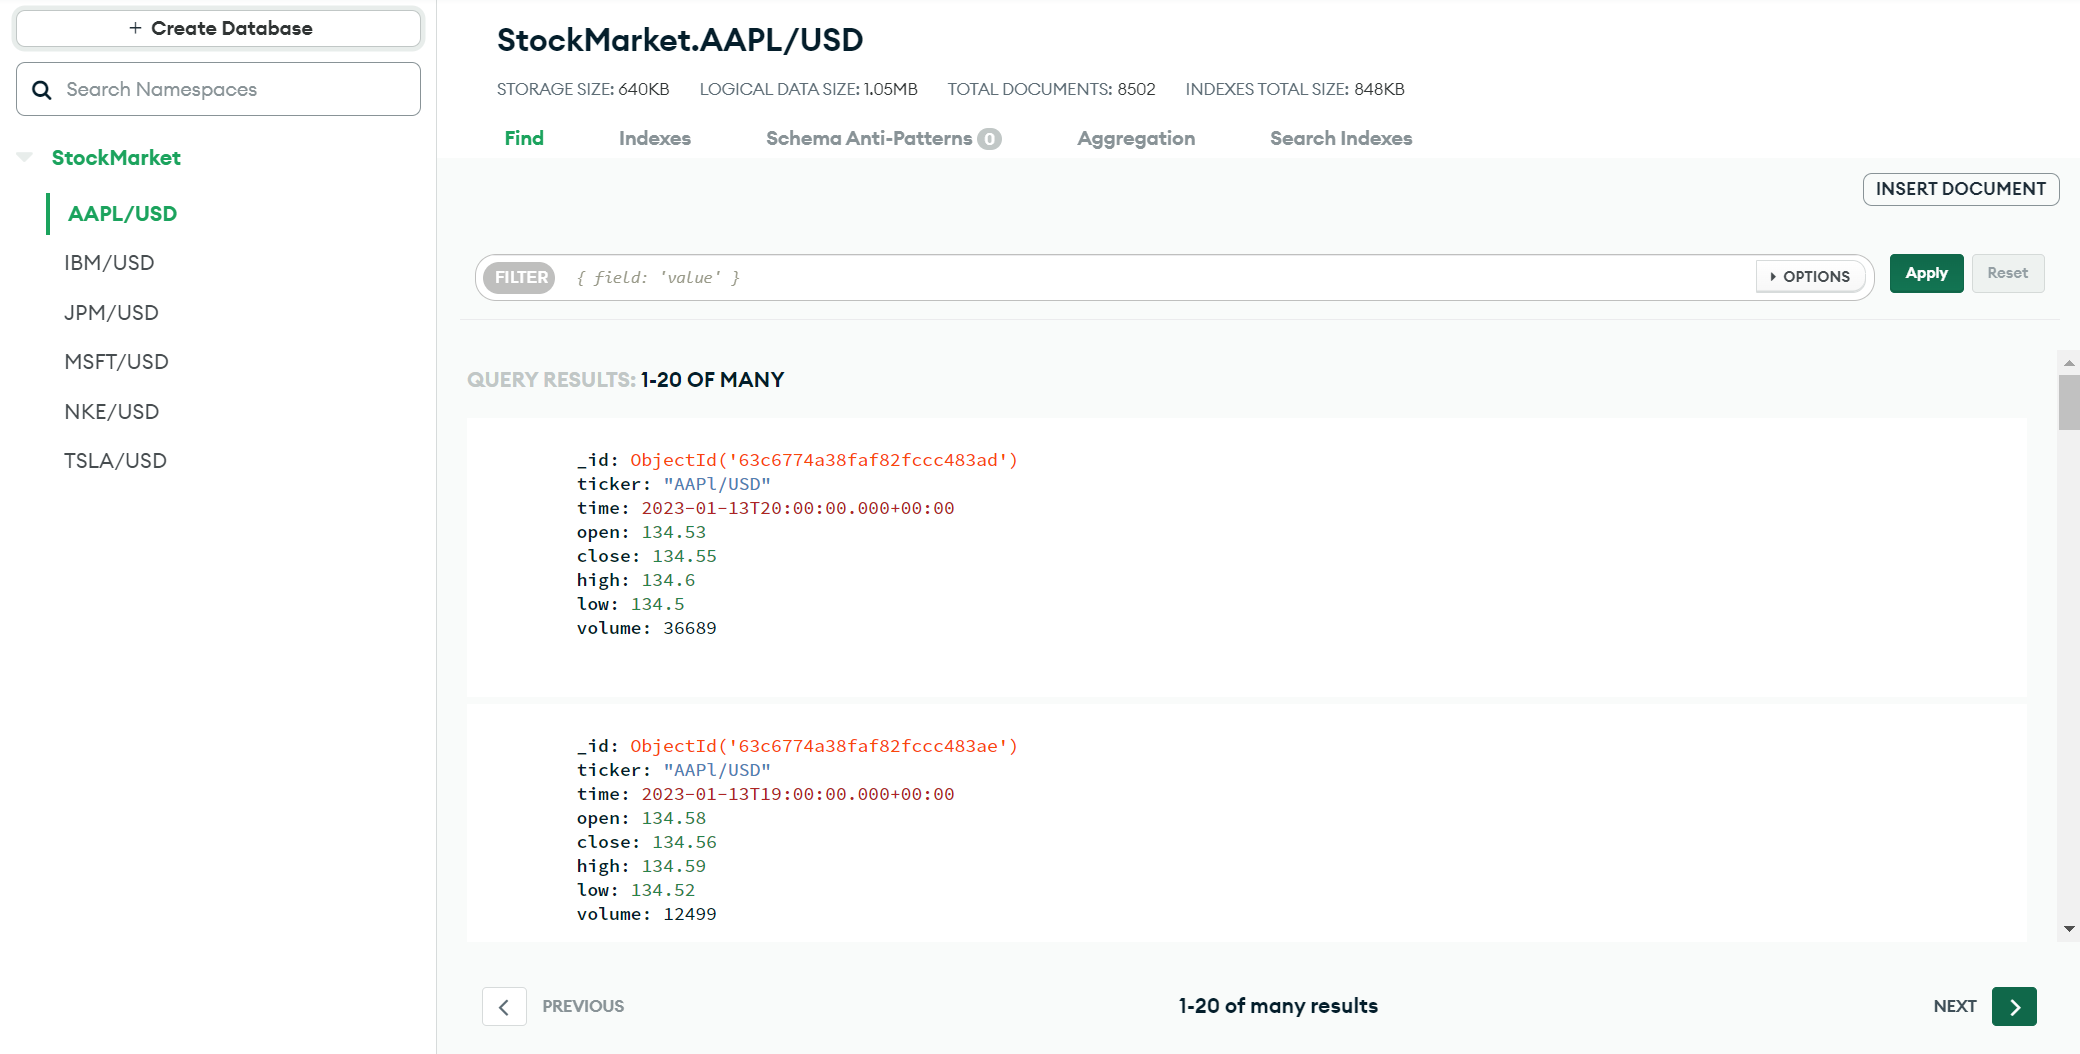
\includegraphics[width=\textwidth]{images/db_example.png}
    \caption{ตัวอย่างข้อมูลตลาดหุ้นในฐานข้อมูล}
\end{figure}
\pagebreak


\subsubsection{การตั้งค่าของตัวชี้วัด}
\begin{figure}[ht]
    \centering
    \subfigure[aroon up]{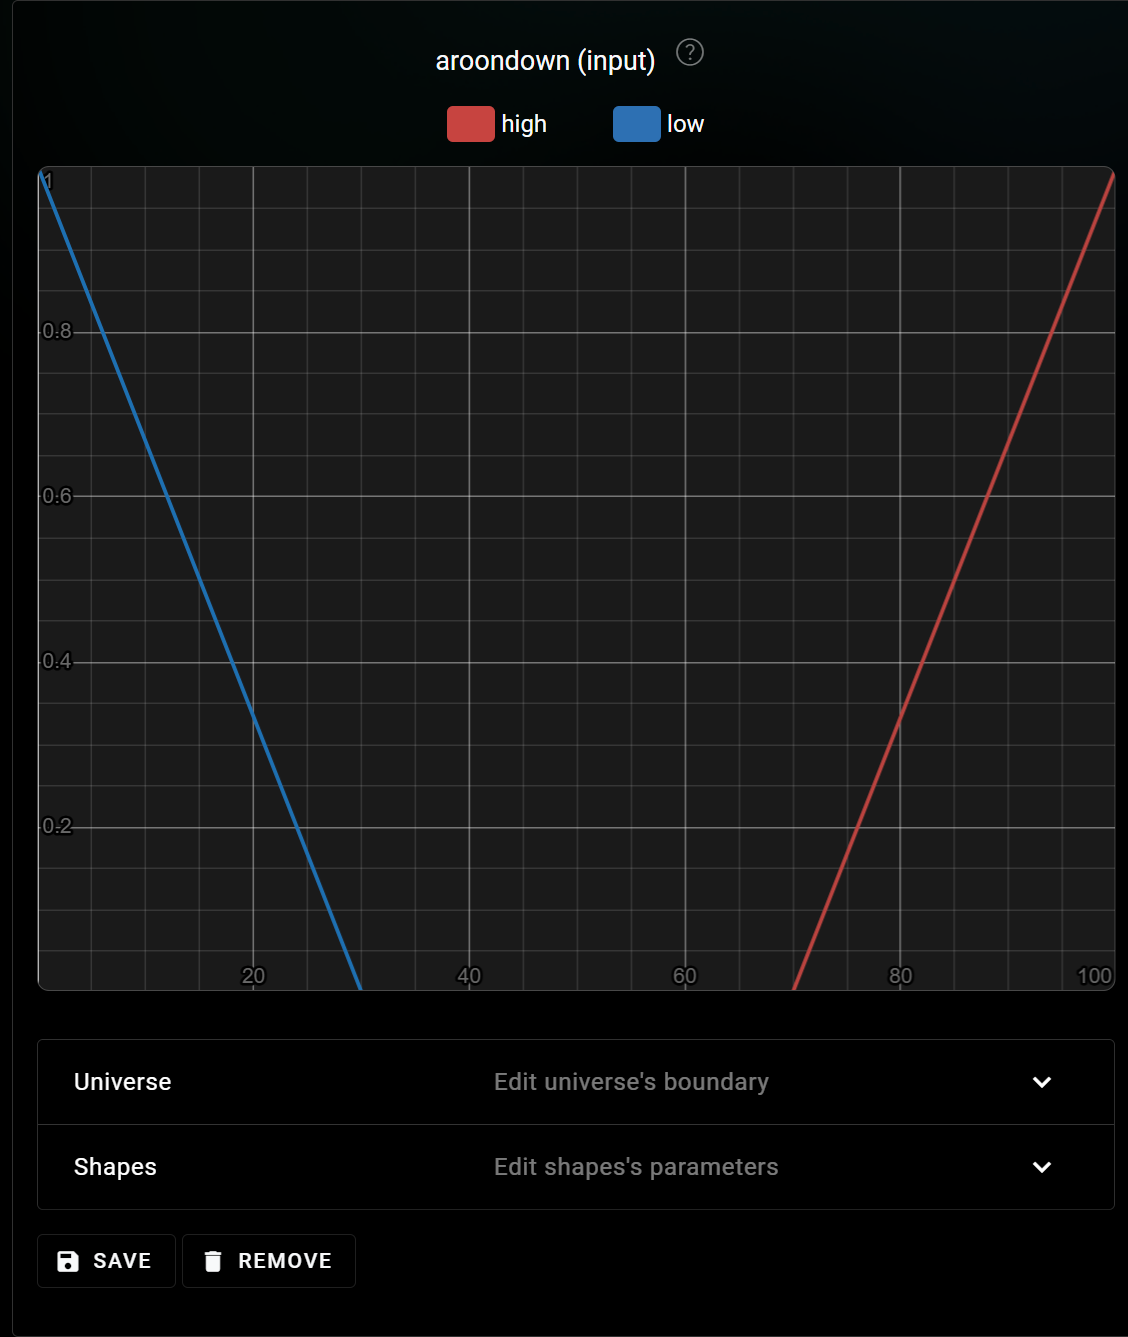
\includegraphics[width=0.4\textwidth]{images/aroon-macd/aroondown.png}}
    \subfigure[aroon down]{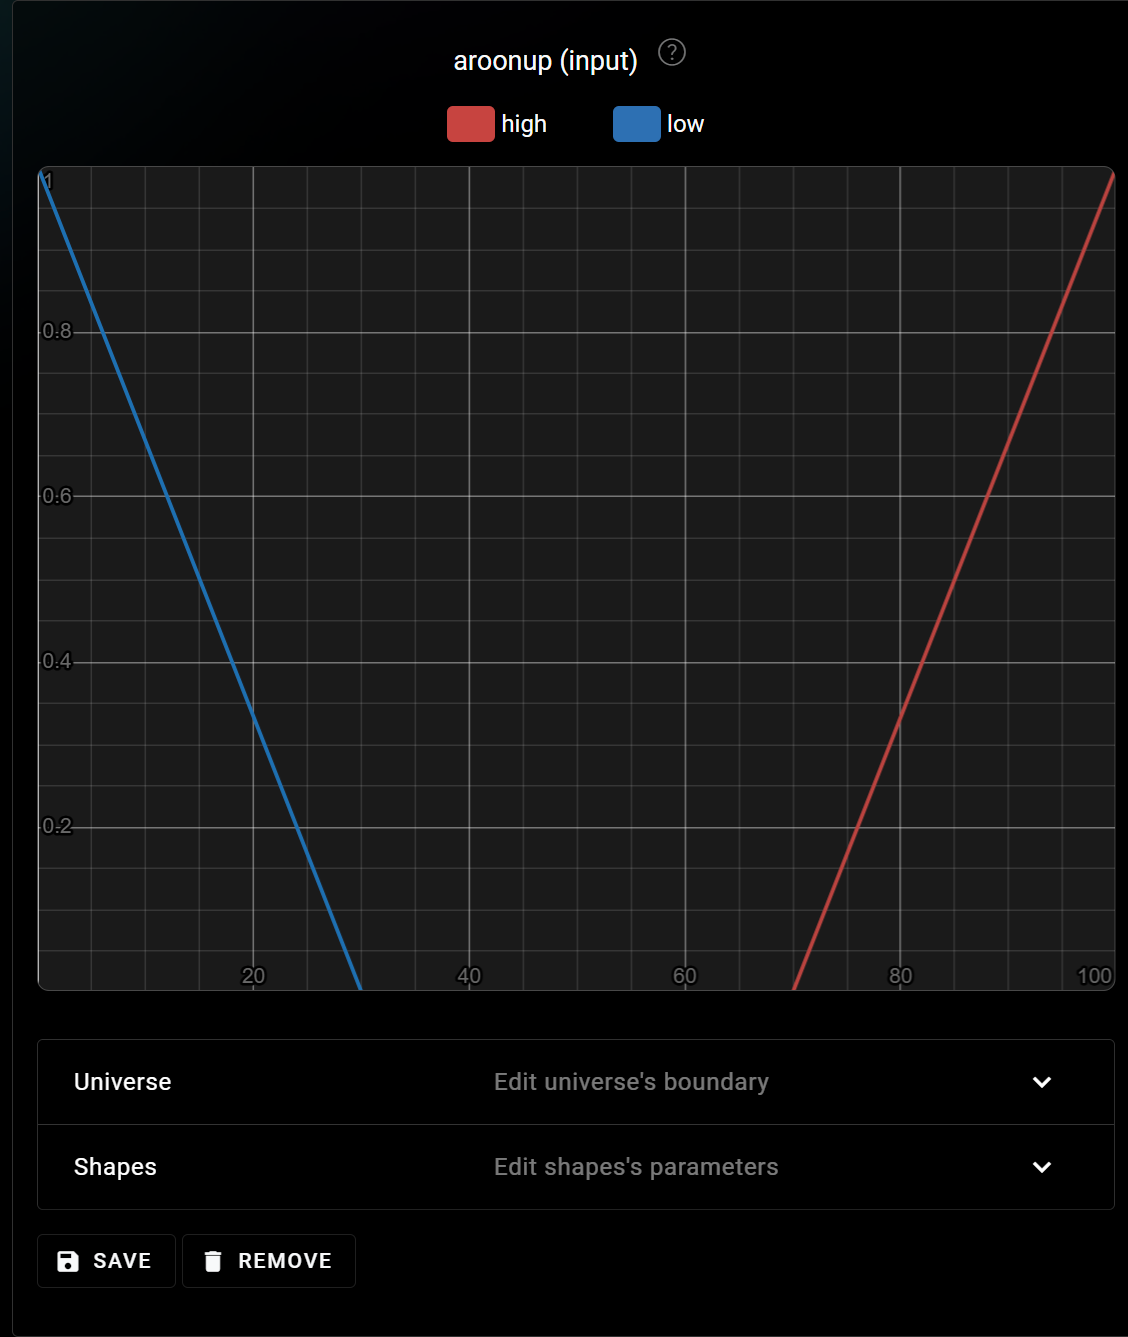
\includegraphics[width=0.4\textwidth]{images/aroon-macd/aroonup.png}}
    \subfigure[macd]{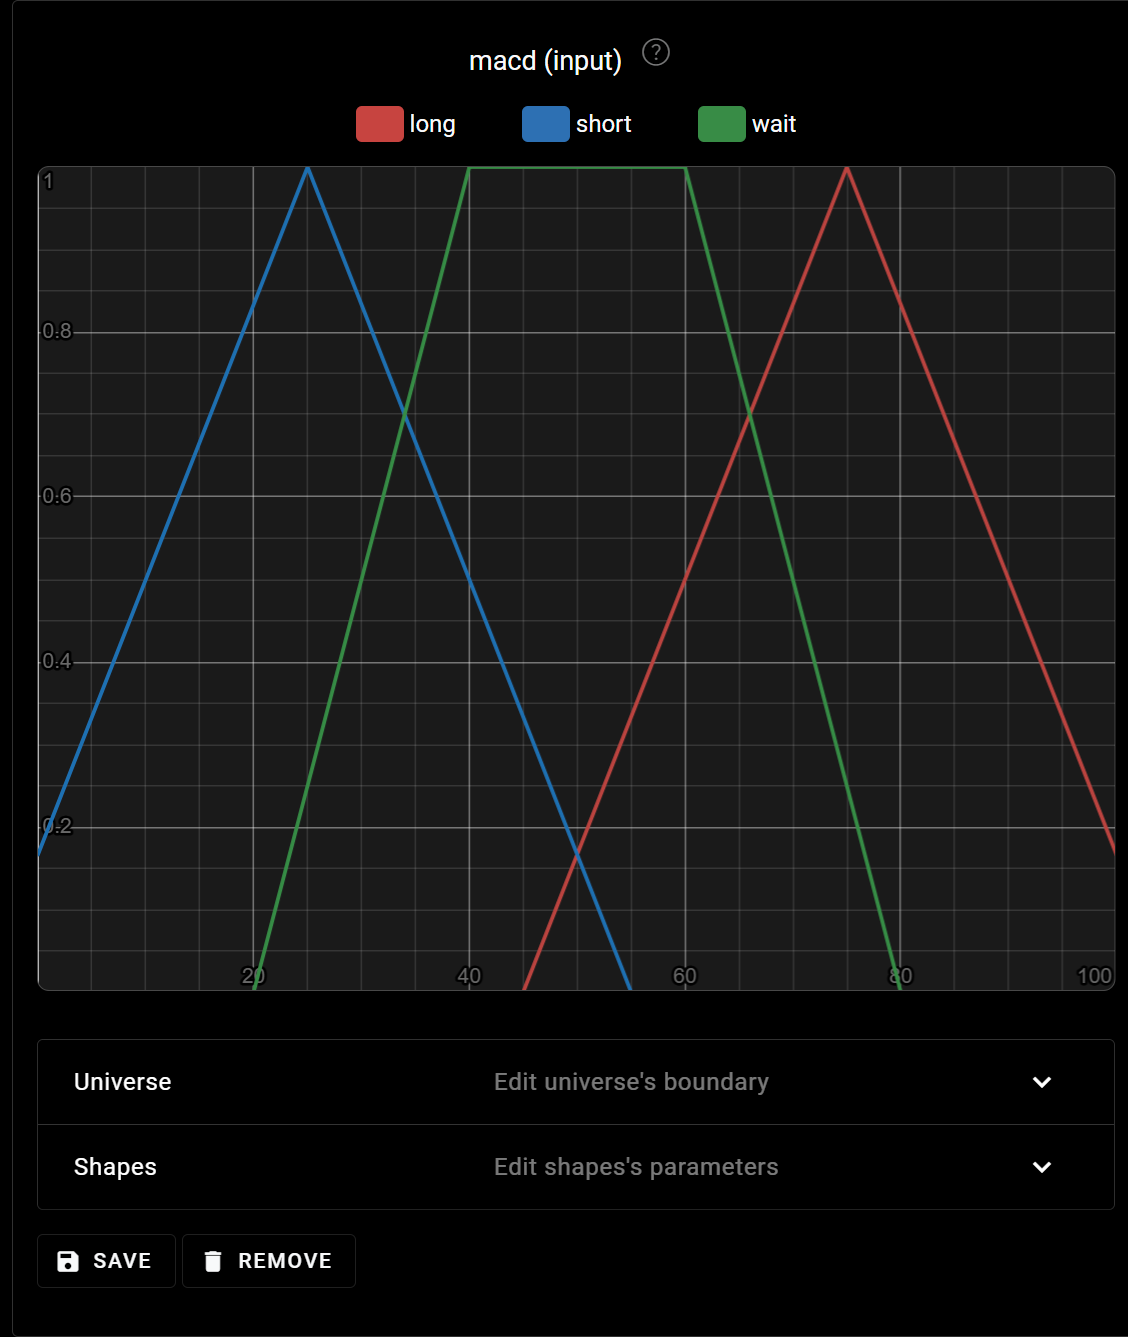
\includegraphics[width=0.4\textwidth]{images/aroon-macd/macd.png}}
    \subfigure[long]{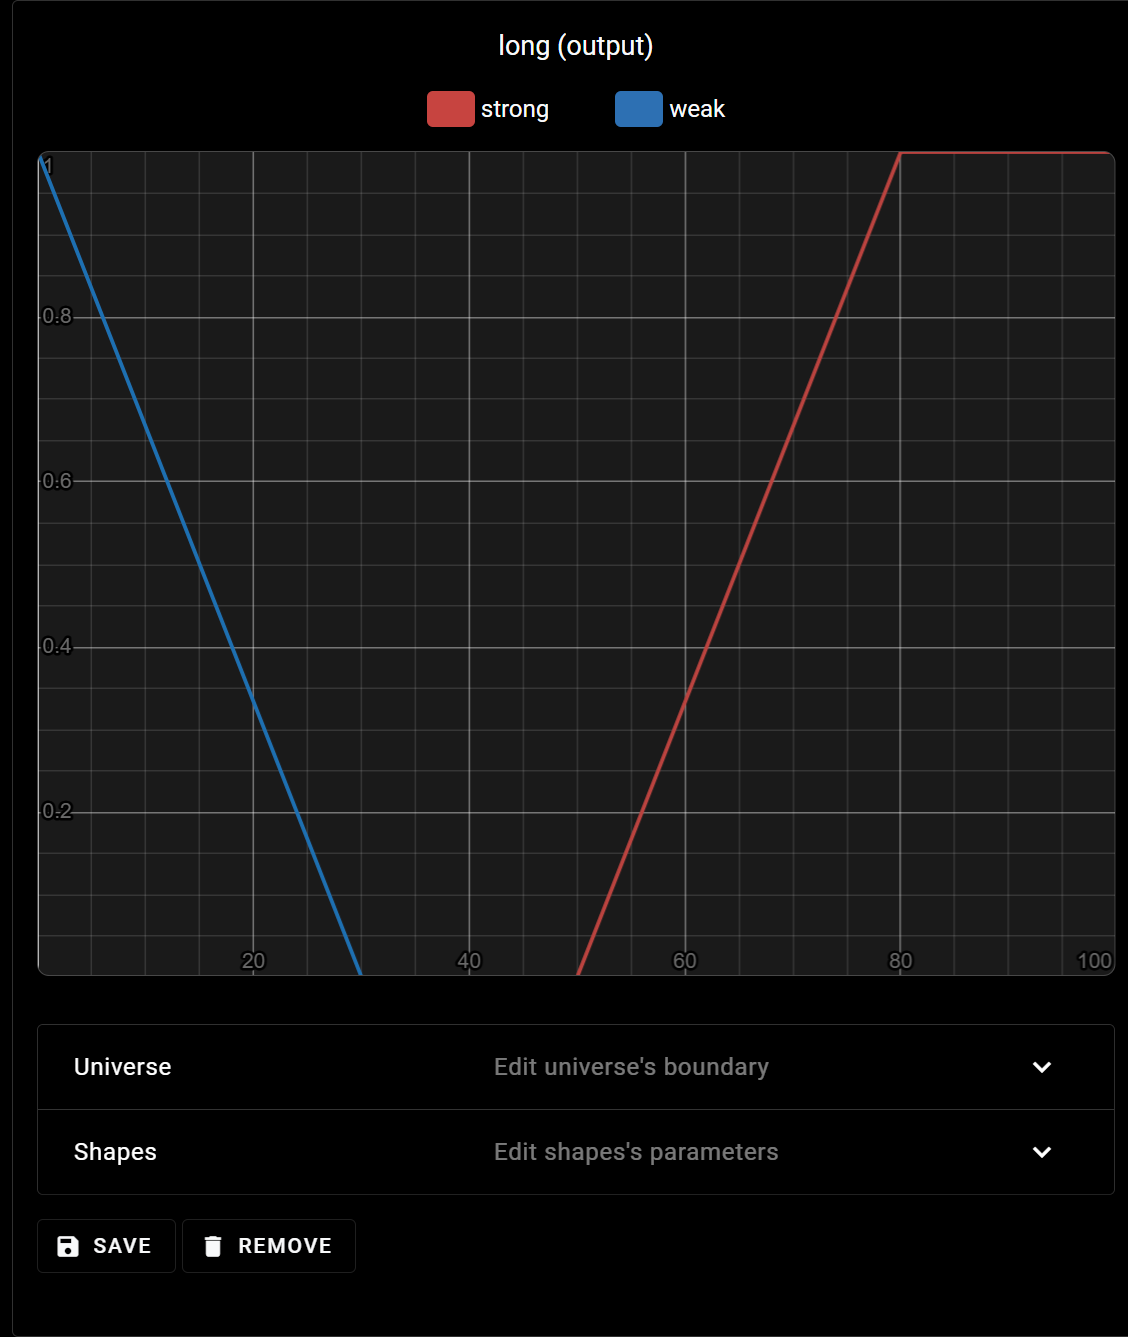
\includegraphics[width=0.4\textwidth]{images/aroon-macd/long.png}}
    \subfigure[short]{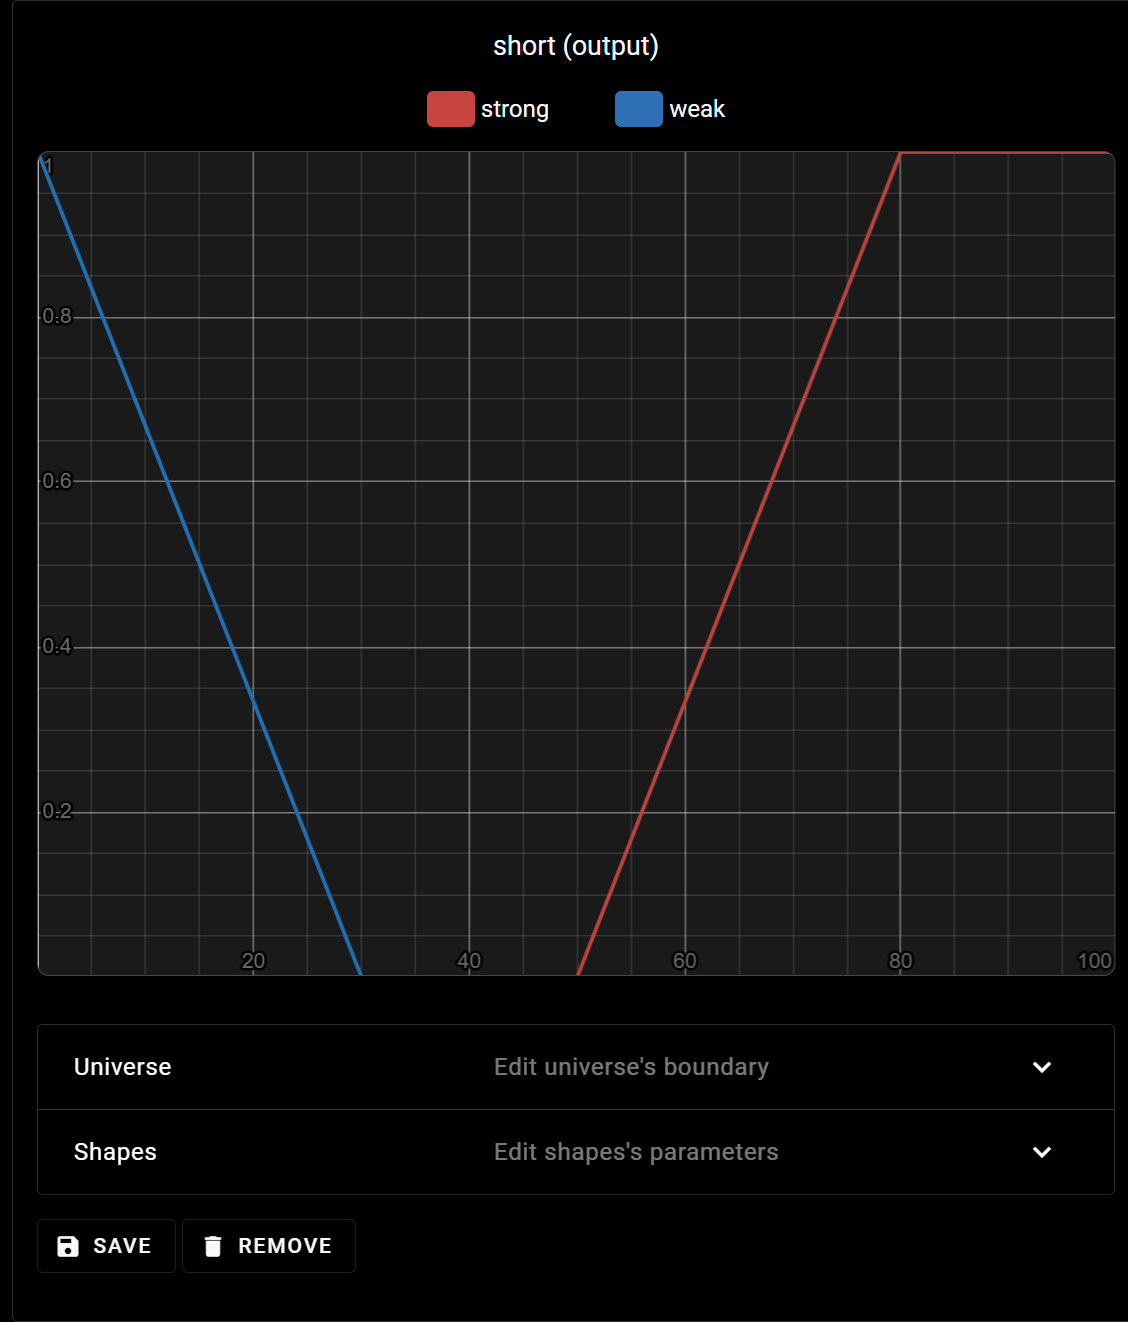
\includegraphics[width=0.4\textwidth]{images/aroon-macd/short.png}}
    \caption{ตัวแปรทางภาษาของตัวชี้วัด AROON-MACD จากในระบบของเรา}
    \label{fig:aroon-macd-lin}
\end{figure}

\begin{figure}[ht]
    \centering
    \subfigure[bollinger band]{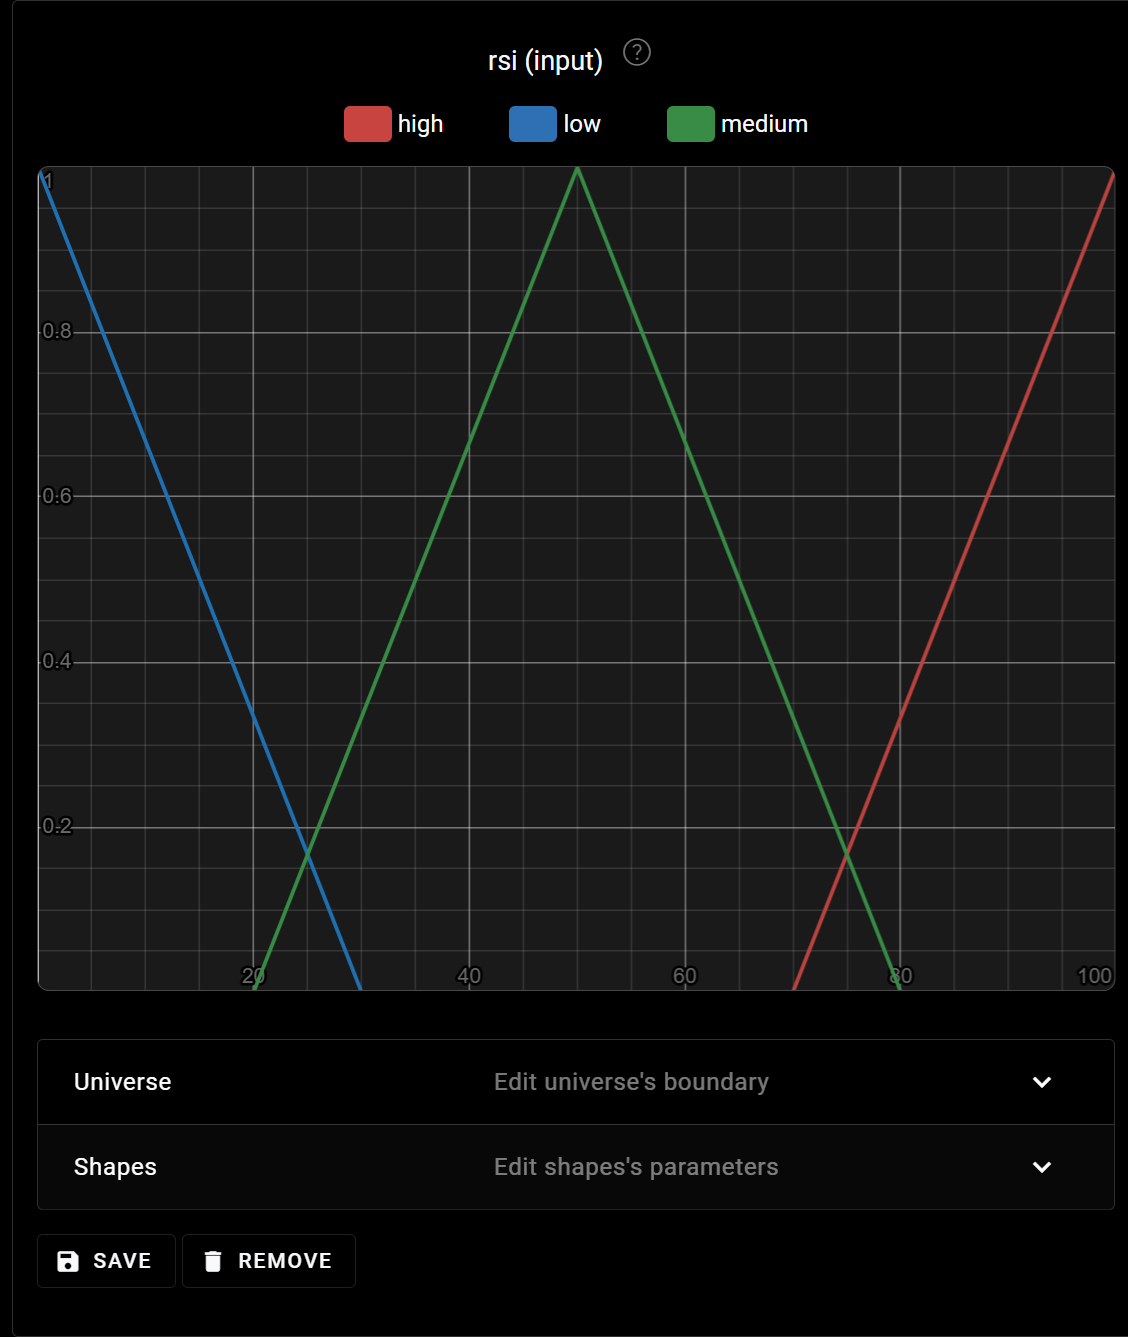
\includegraphics[width=0.4\textwidth]{images/rsi-bb/rsi.png}}
    \subfigure[rsi]{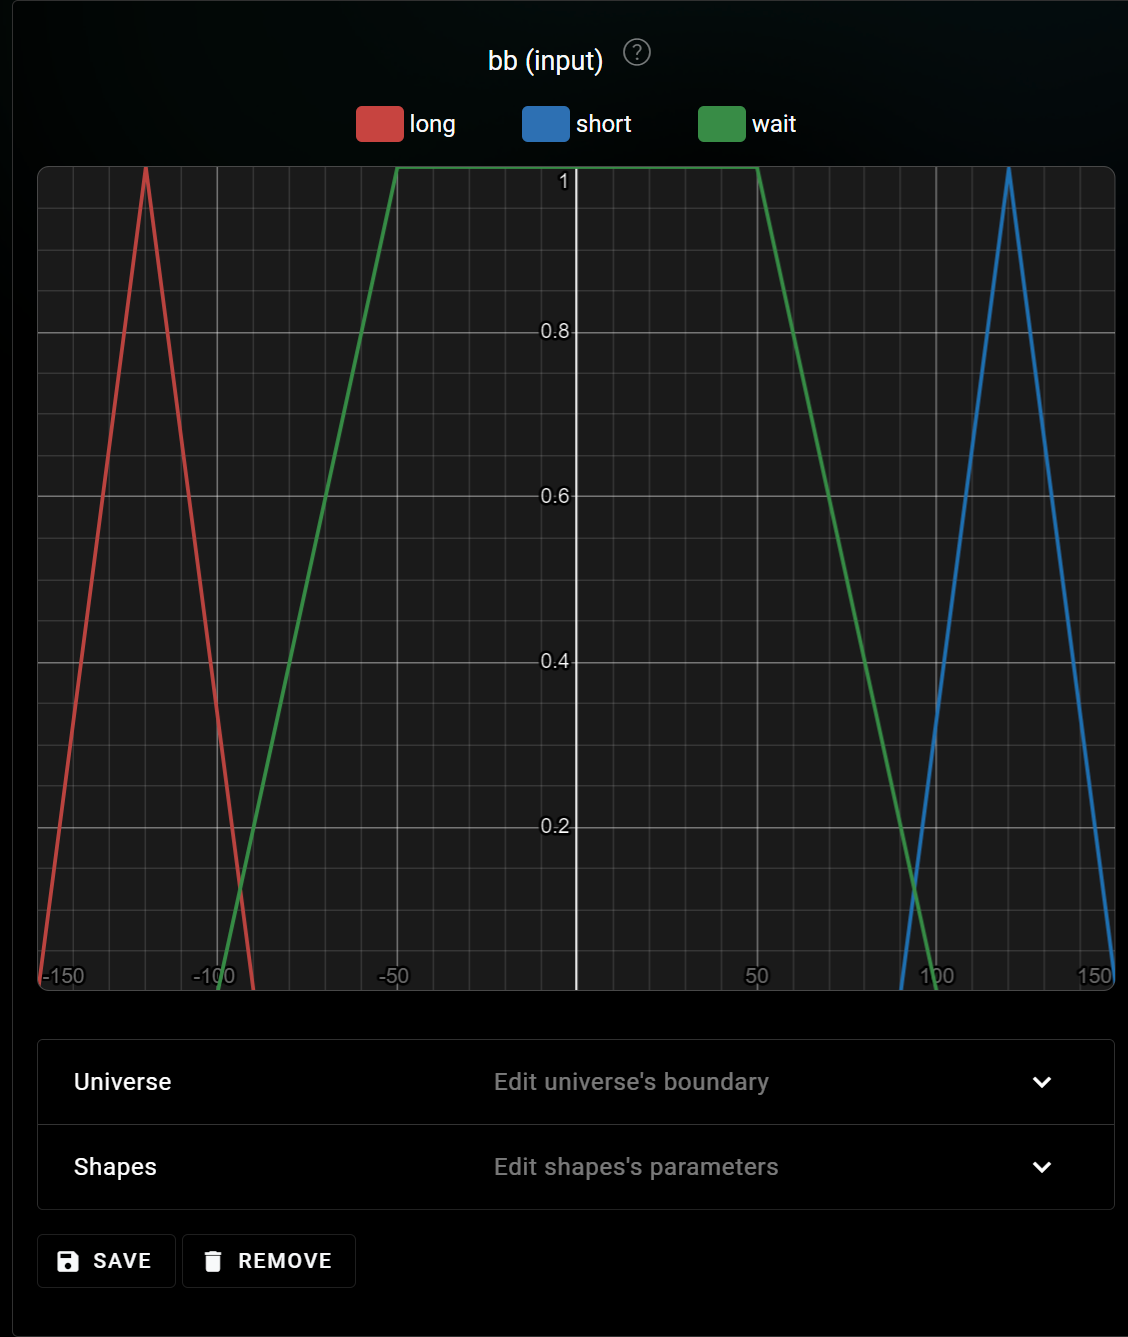
\includegraphics[width=0.4\textwidth]{images/rsi-bb/bb.png}}
    \subfigure[long]{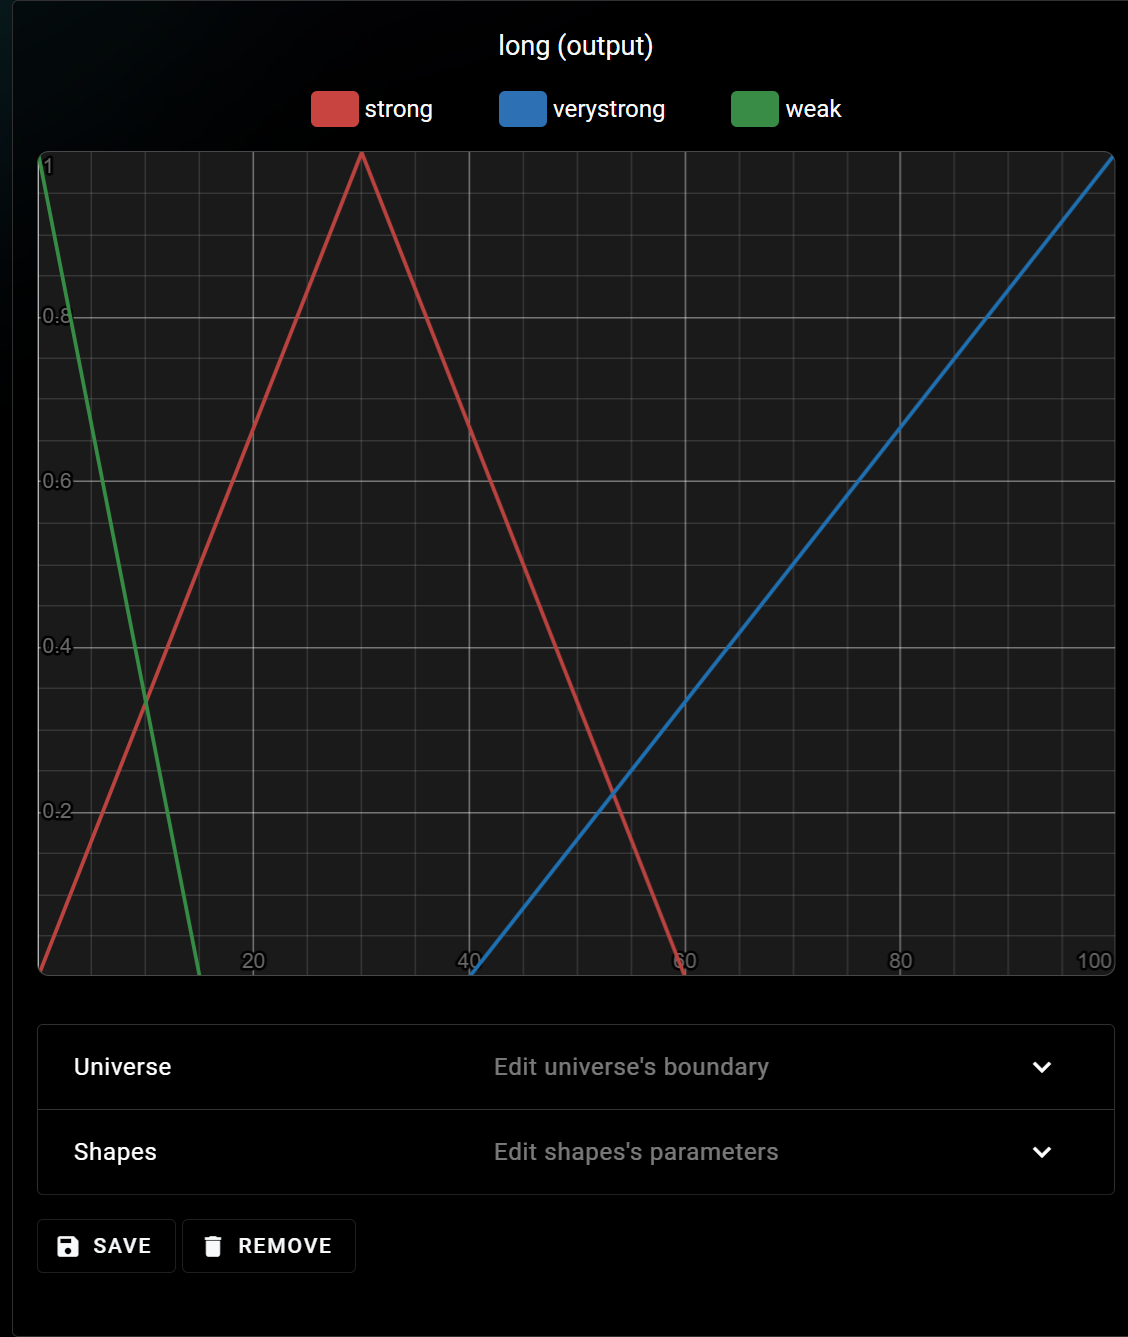
\includegraphics[width=0.4\textwidth]{images/rsi-bb/long.png}}
    \subfigure[short]{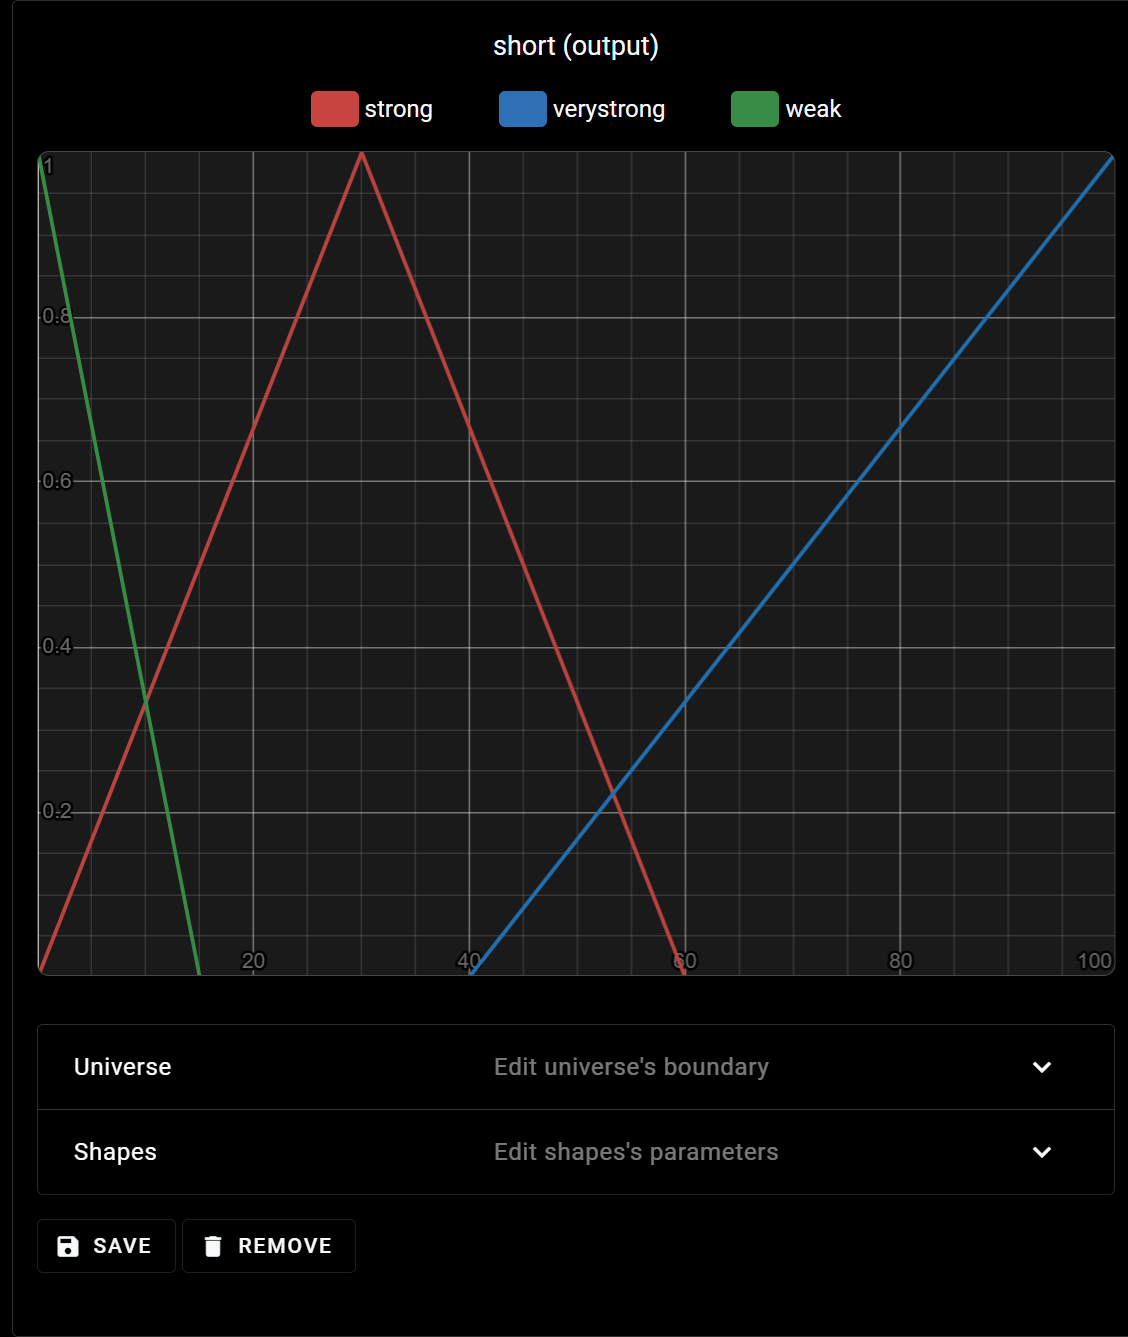
\includegraphics[width=0.4\textwidth]{images/rsi-bb/short.png}}
    \caption{ตัวแปรทางภาษาของตัวชี้วัด RSI-BB จากในระบบของเรา}
    \label{fig:rsi-bb-lin}
\end{figure}

\begin{figure}[ht]
    \centering
    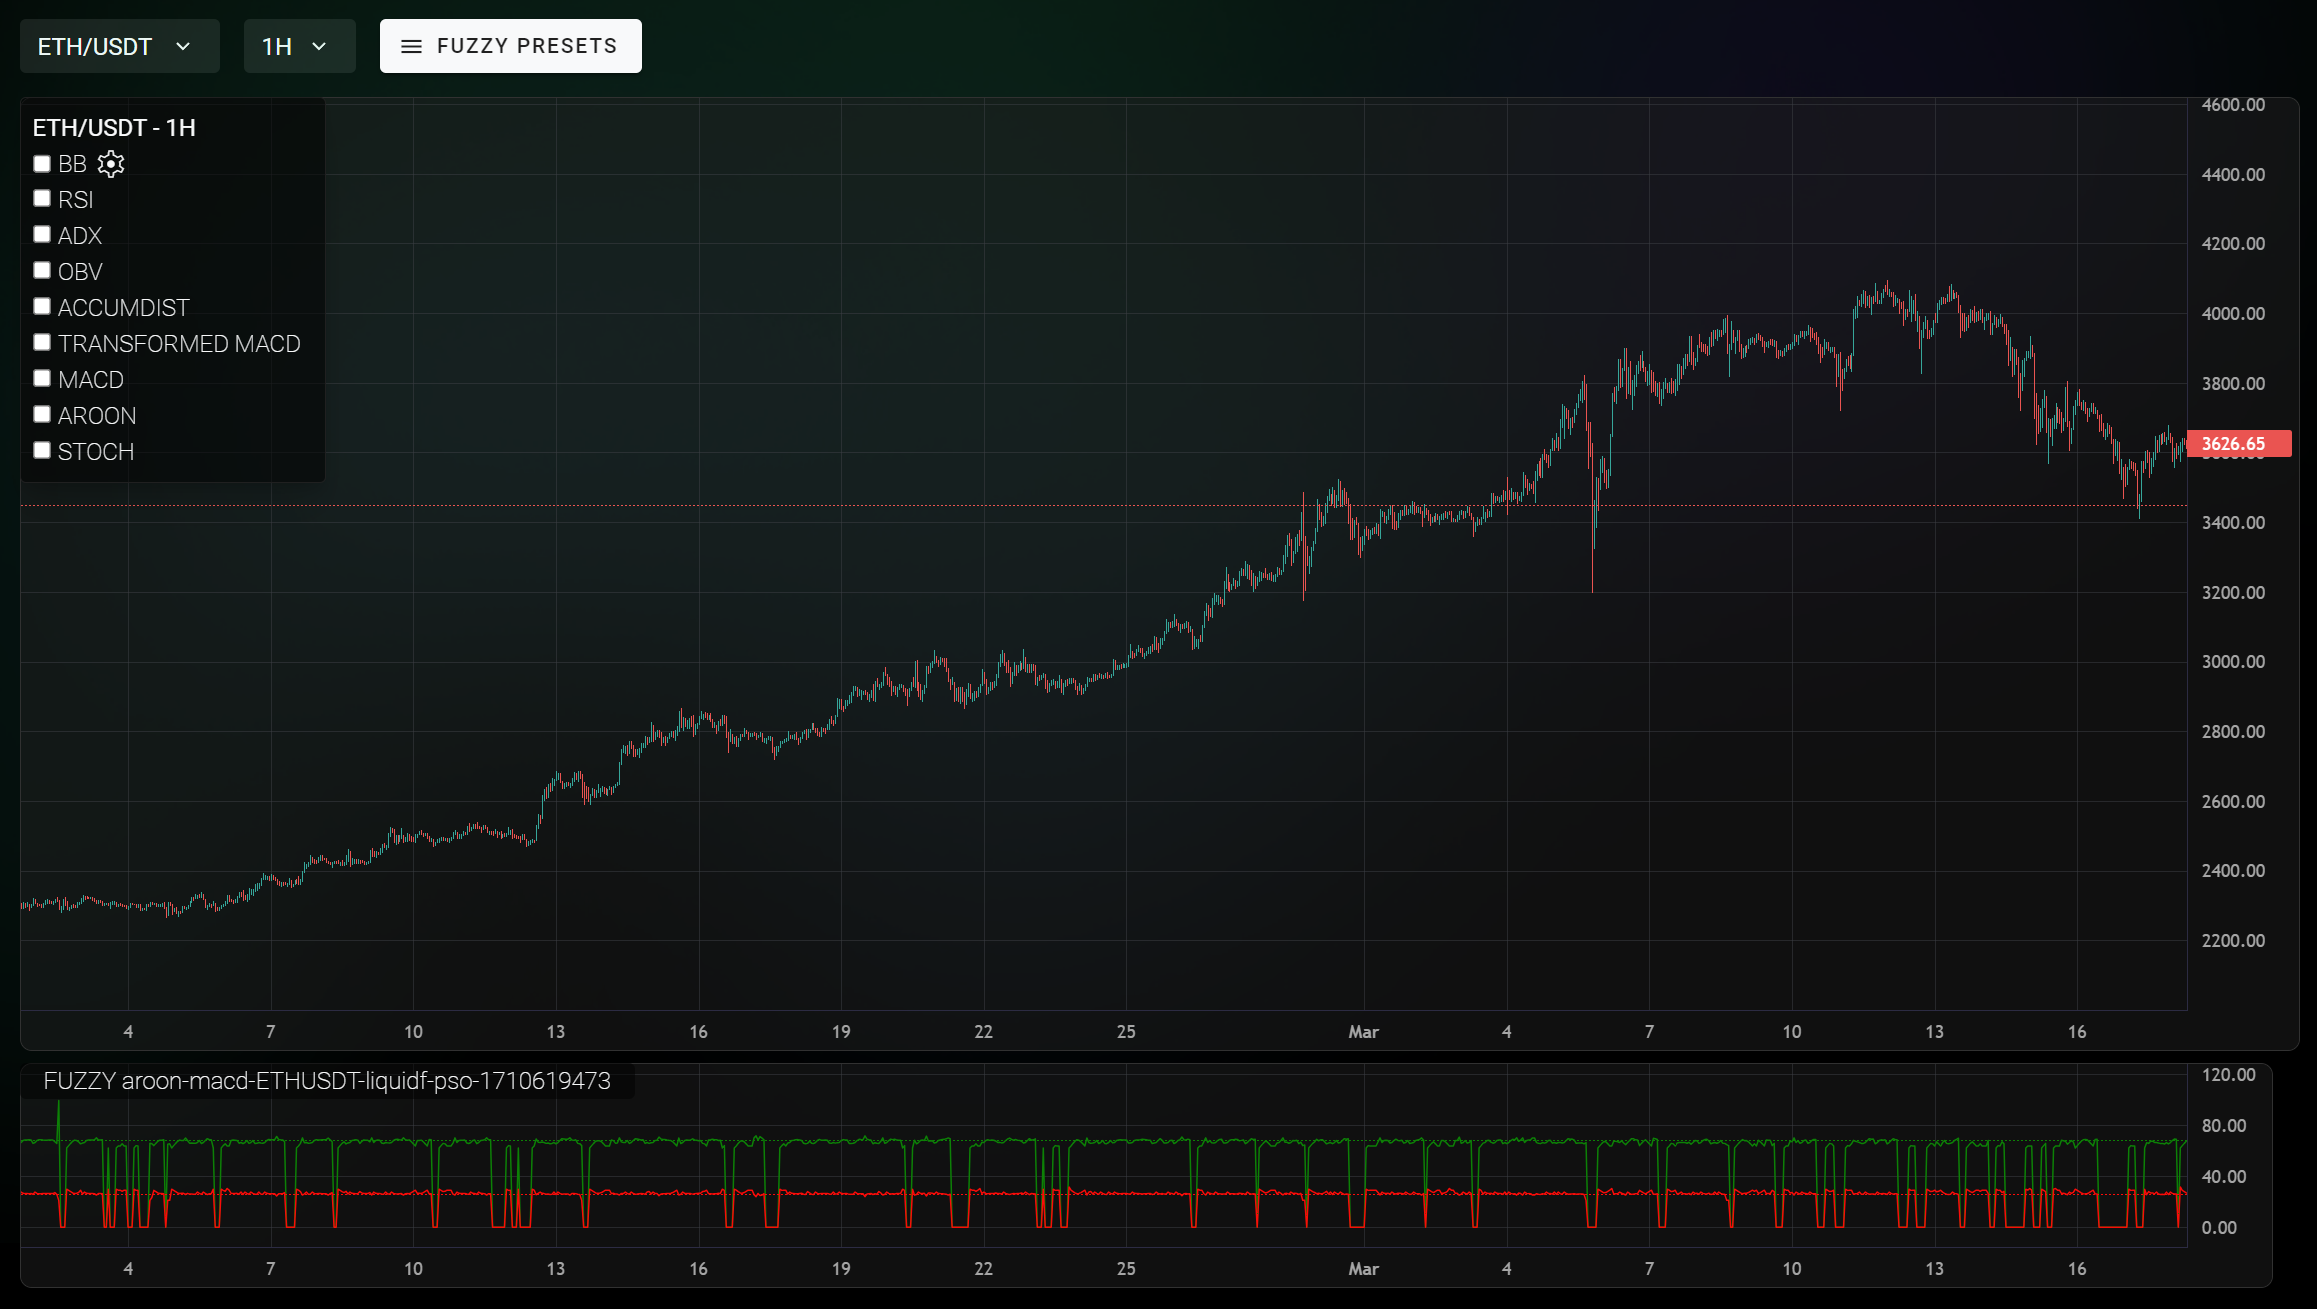
\includegraphics[width=0.4\textwidth]{images/aroon-macd/example.png}
    \caption{ตัวอย่างผลลัพธ์ของ AROON-MACD แบบ Fuzzy C PSO}
    \label{fig:aroon-macd-example}
\end{figure}

\subsubsection{ผลลัพธ์จากการใช้ PSO ฝึกสอน}
\begin{figure}[ht]
    \centering
    \subfigure[]{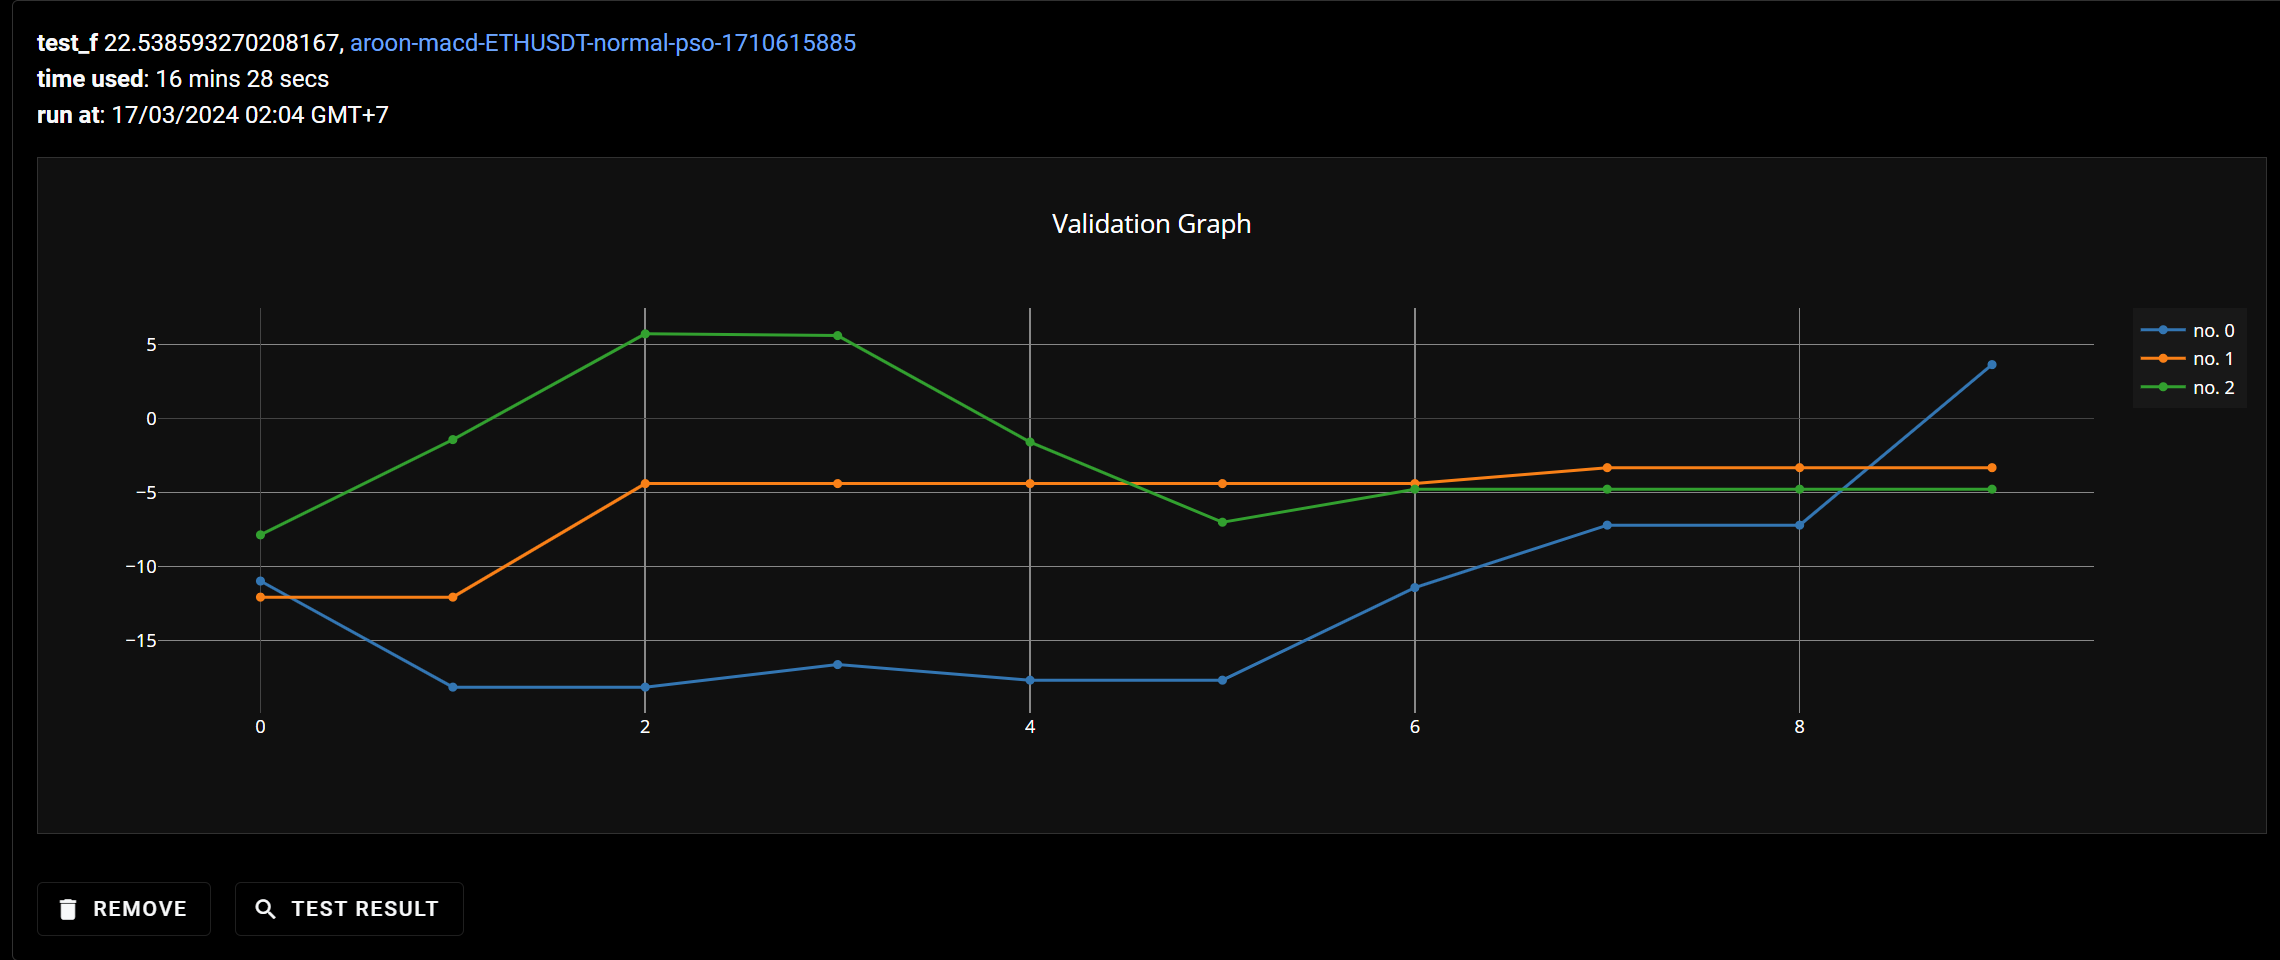
\includegraphics[width=0.5\textwidth]{images/pso/aroon-macd/eth-normal.png}}
    \subfigure[]{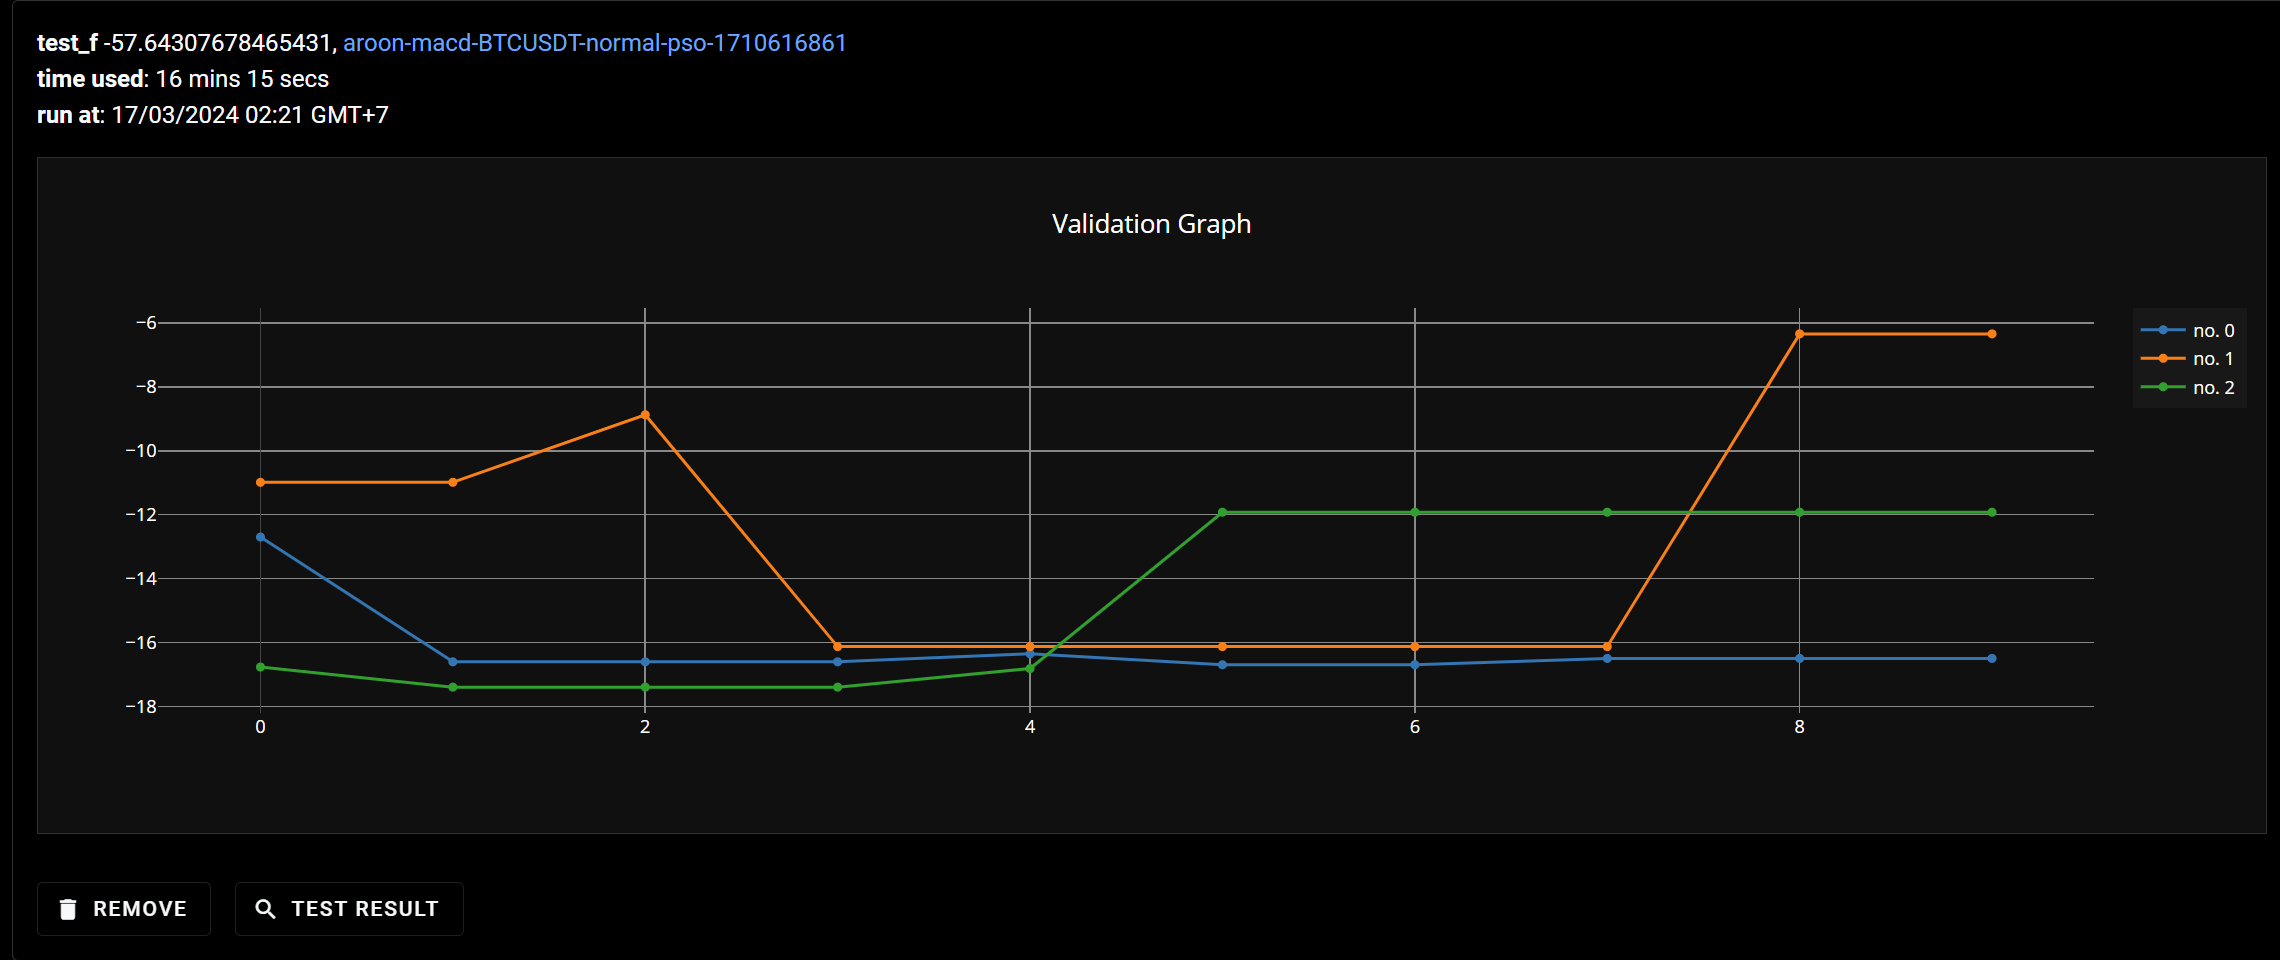
\includegraphics[width=0.5\textwidth]{images/pso/aroon-macd/btc-normal.png}}
    \subfigure[]{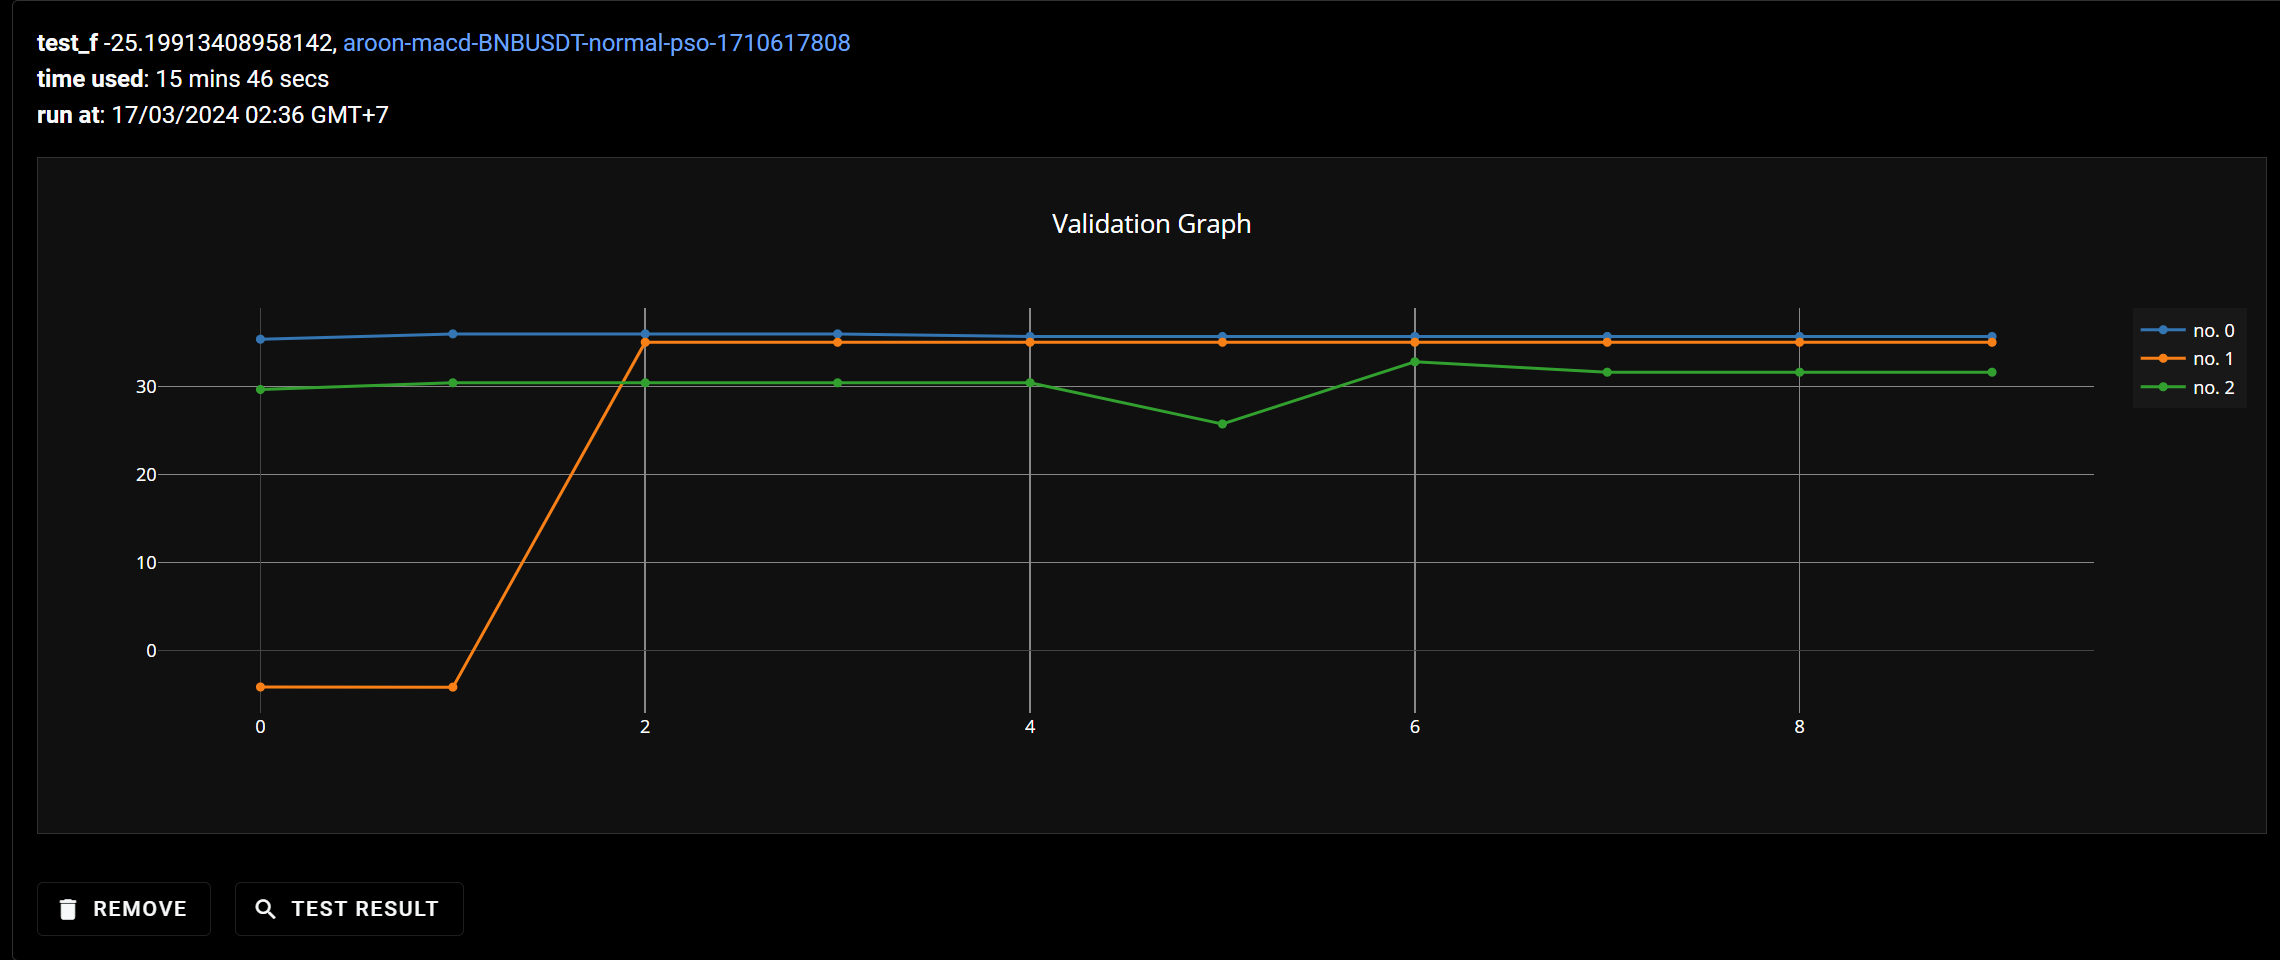
\includegraphics[width=0.5\textwidth]{images/pso/aroon-macd/bnb-normal.png}}
    \subfigure[]{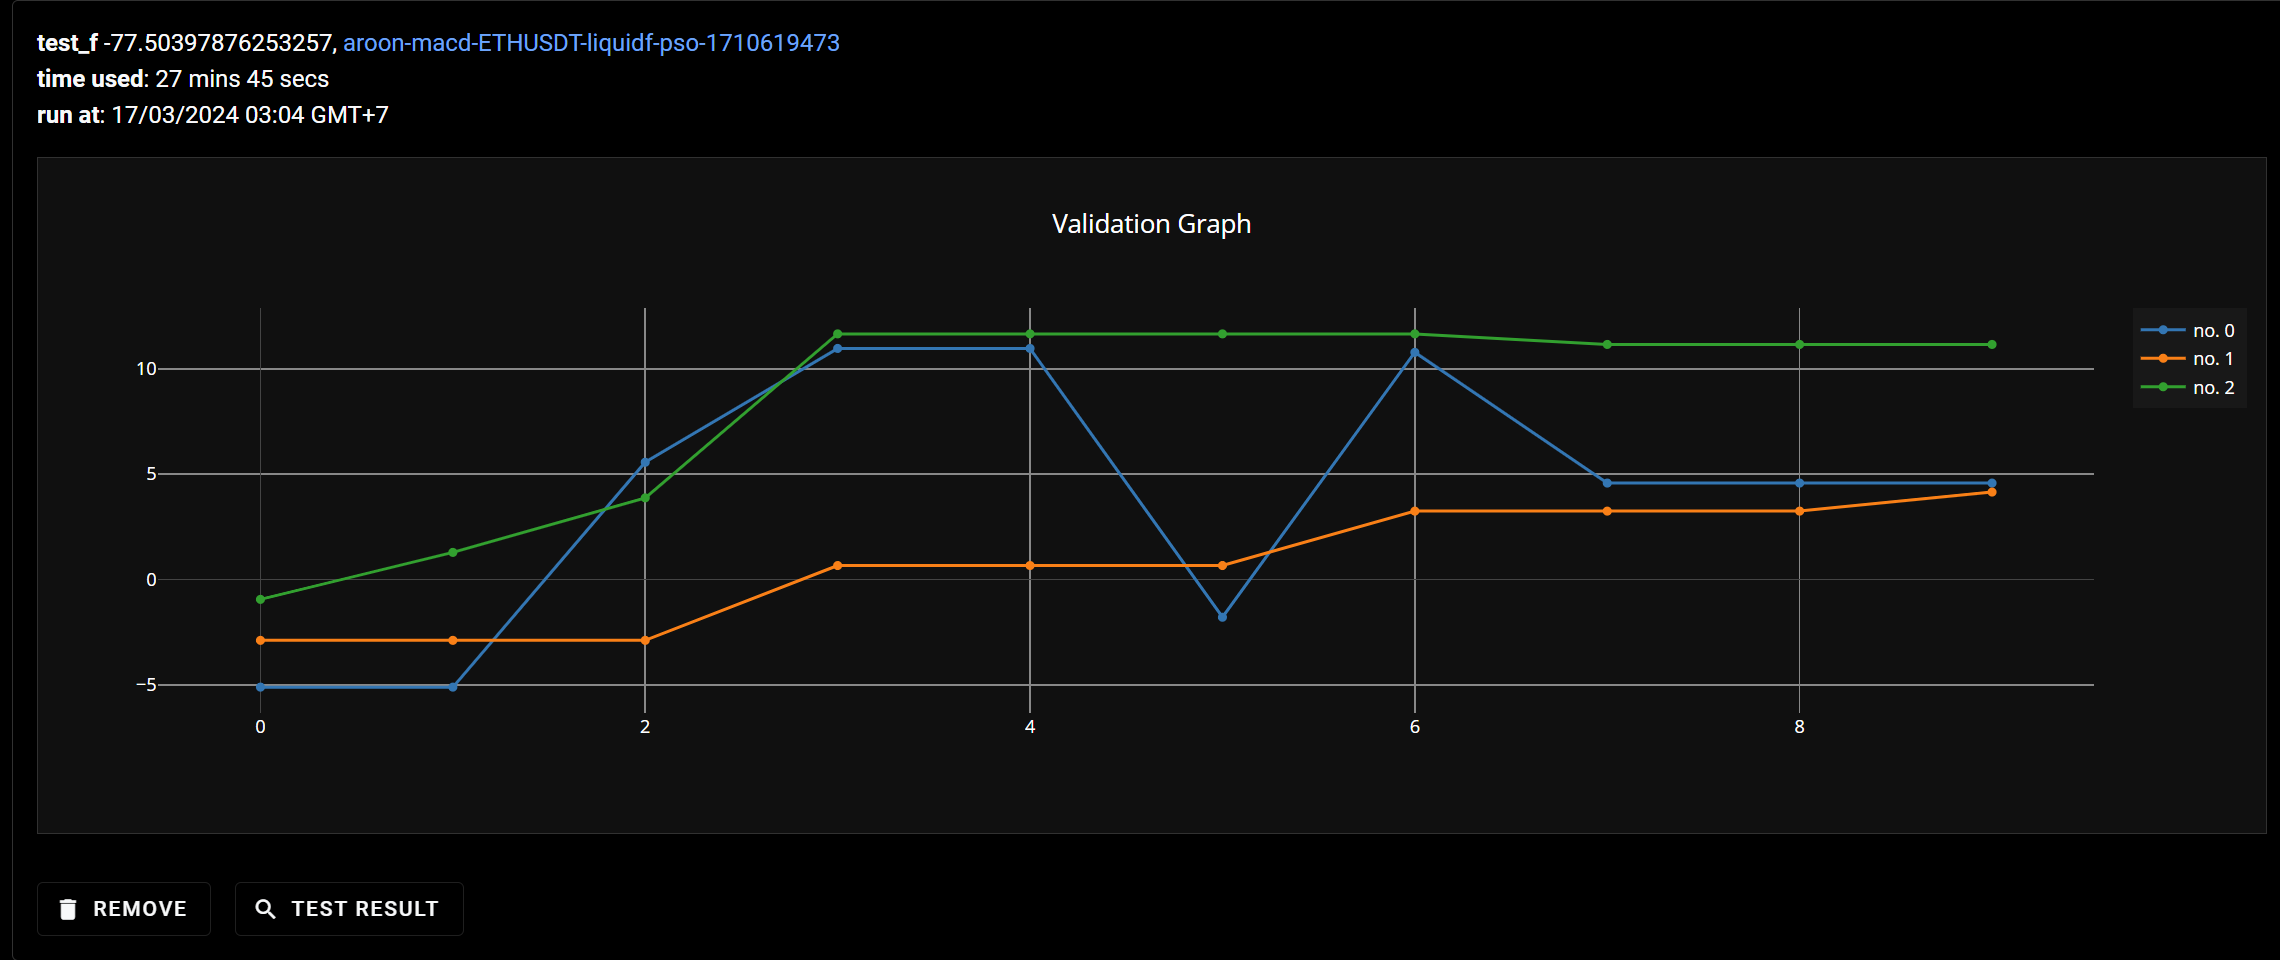
\includegraphics[width=0.5\textwidth]{images/pso/aroon-macd/eth-liquid.png}}
    \subfigure[]{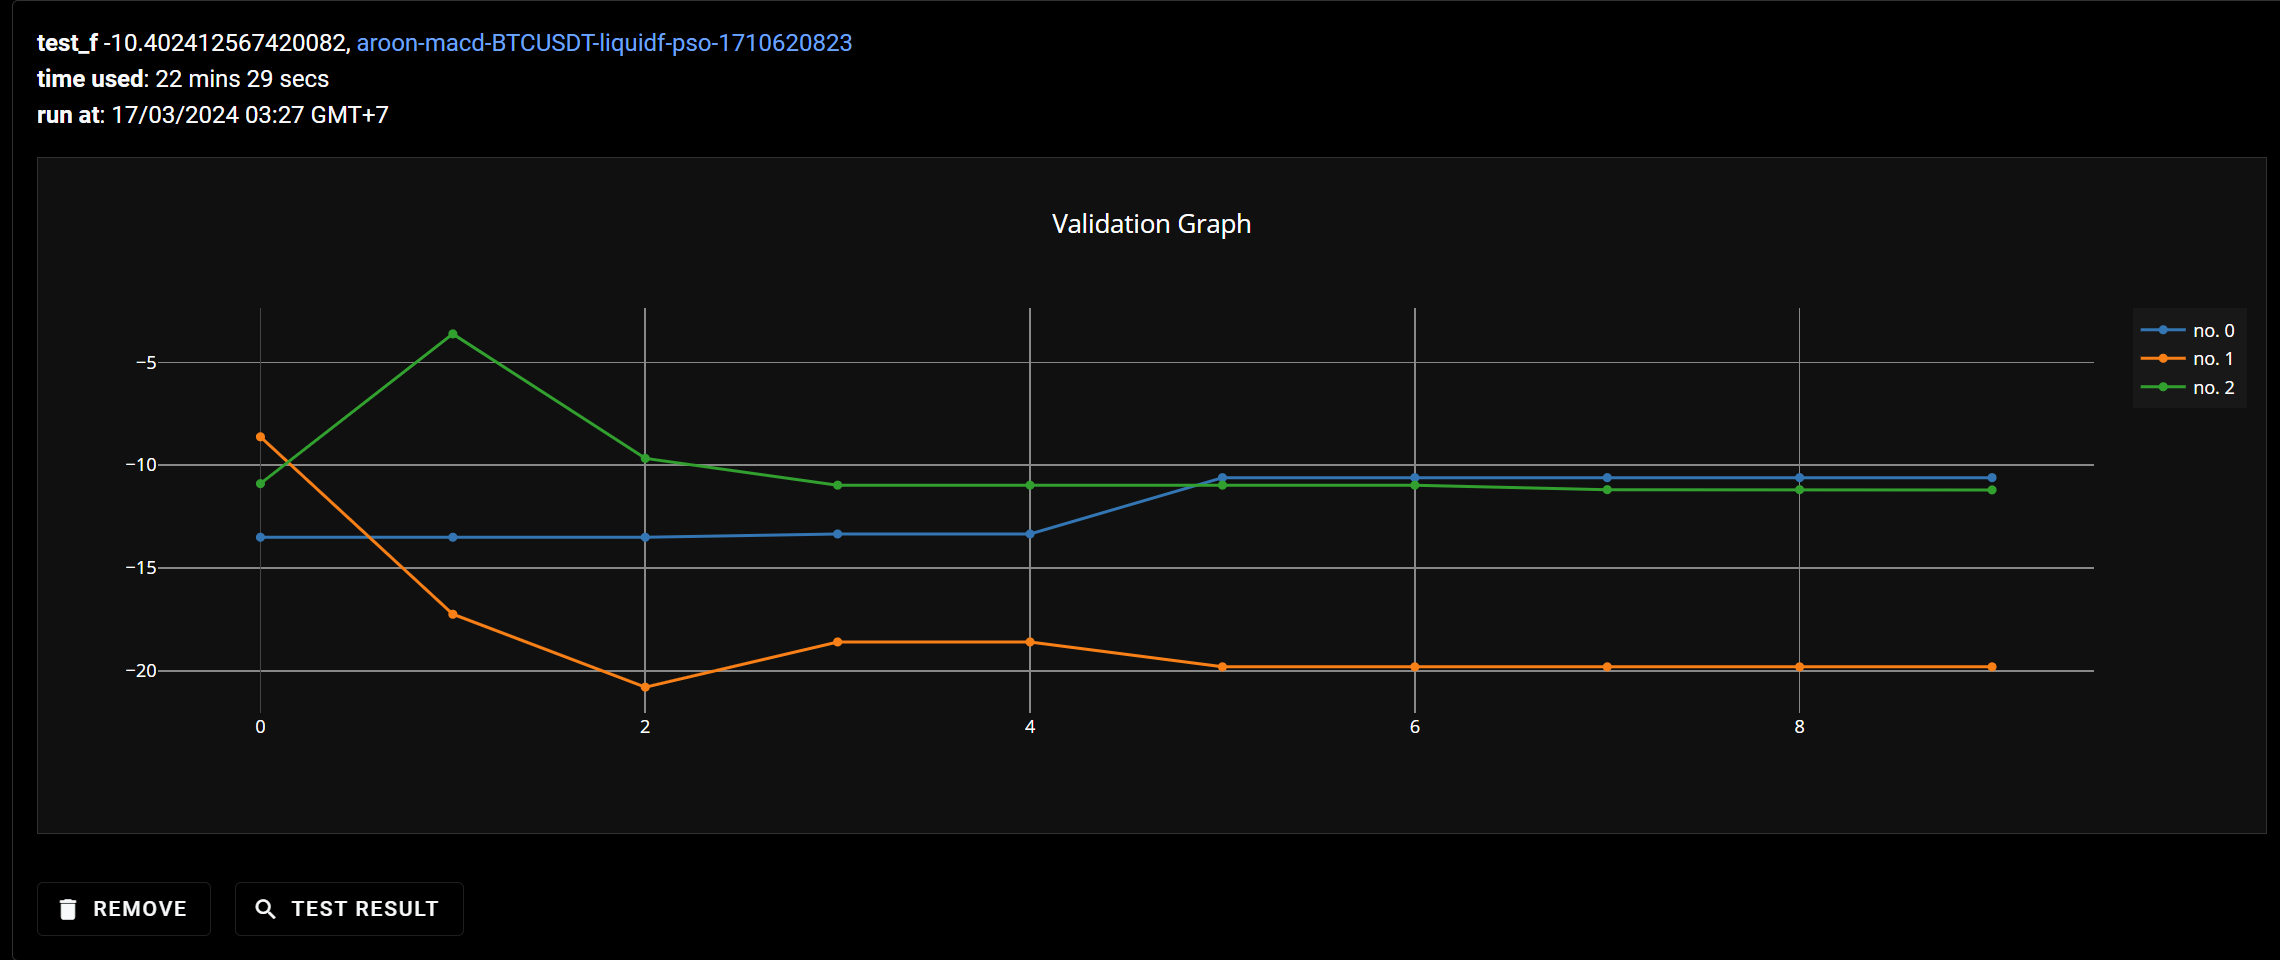
\includegraphics[width=0.5\textwidth]{images/pso/aroon-macd/btc-liquid.png}}
    \subfigure[]{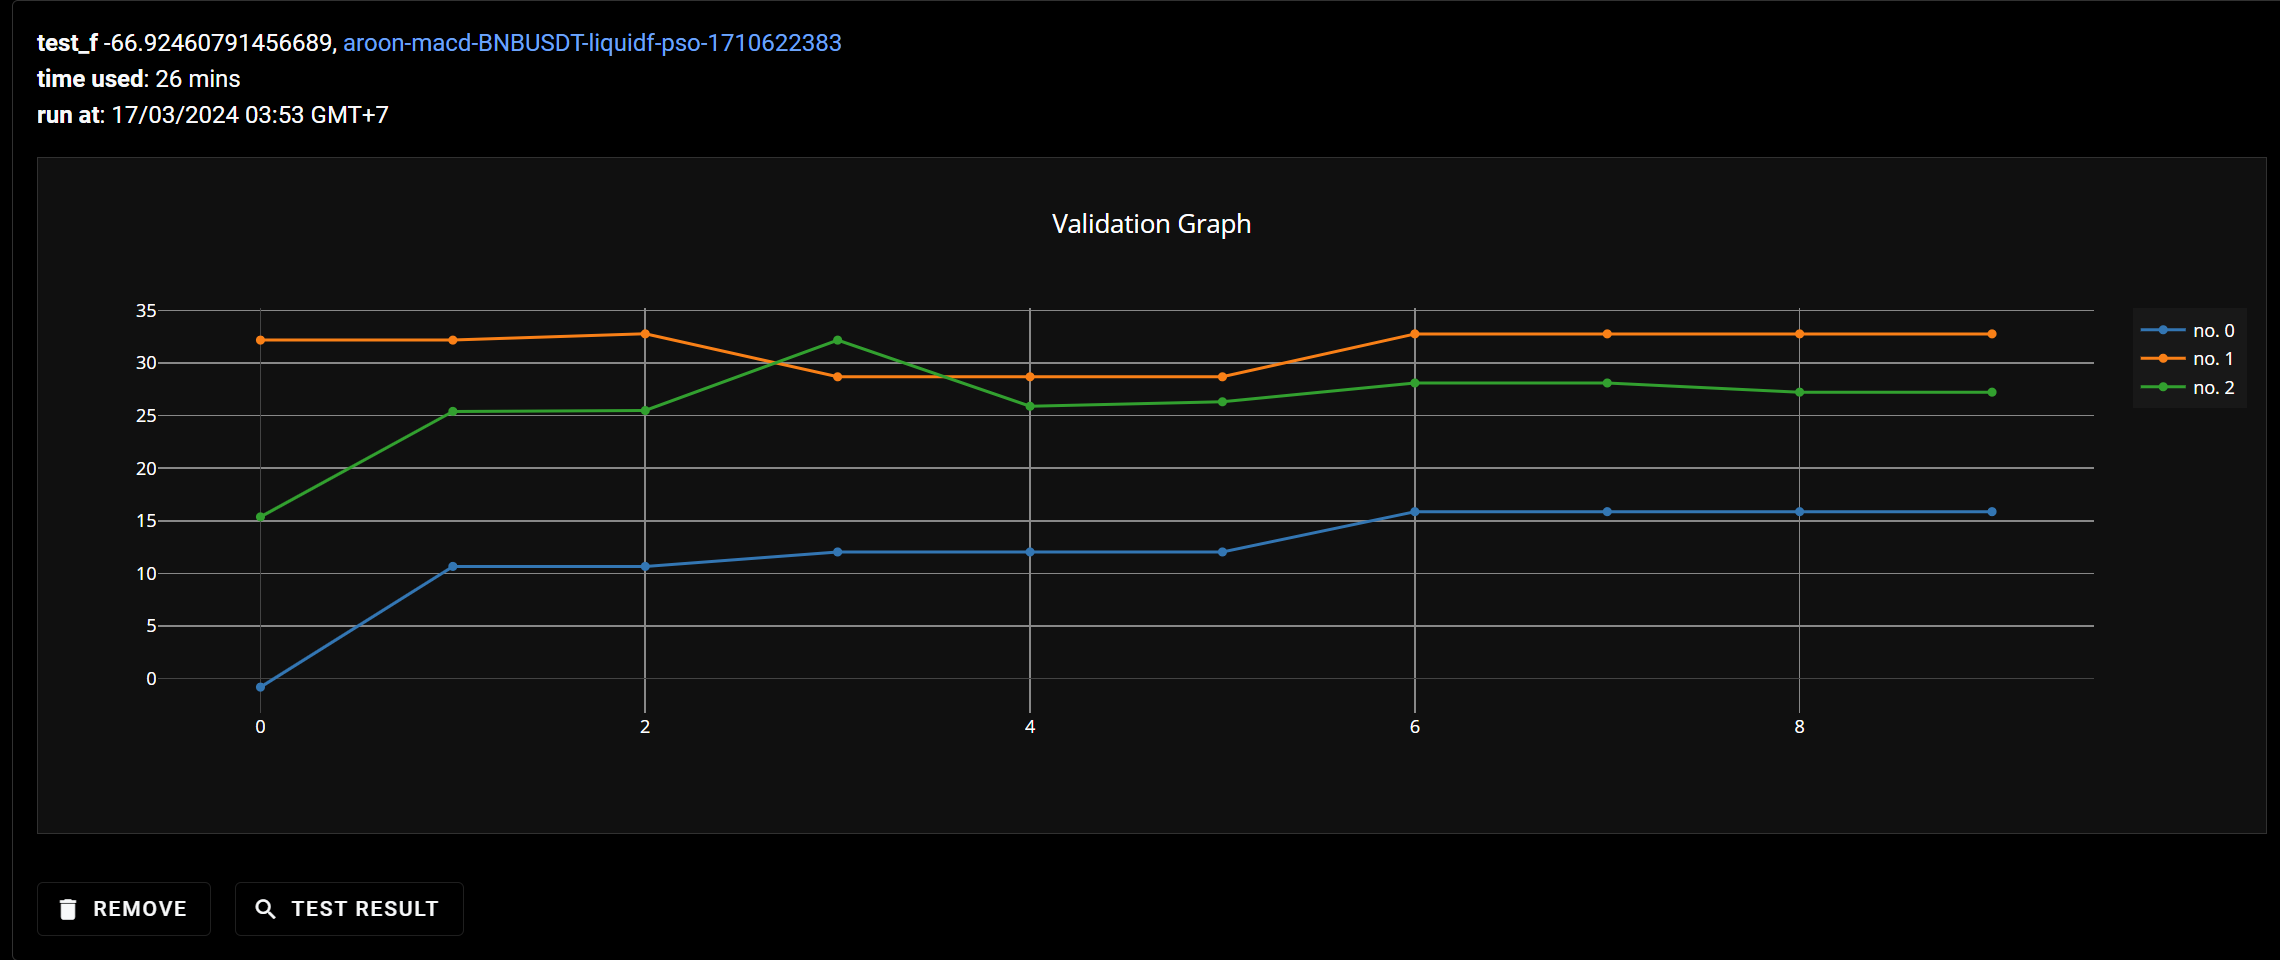
\includegraphics[width=0.5\textwidth]{images/pso/aroon-macd/bnb-liquid.png}}
    \caption{}
\end{figure}

\ifproject
%% Display glossary (optional) -- need glossary option.
\ifglossary\glossarypage\fi

%% Display index (optional) -- need idx option.
\ifindex\indexpage\fi

\begin{biosketch}
\begin{center}
  \includegraphics[width=1.5in]{mugshot.jpg}
\end{center}
Your biosketch goes here. Make sure it sits inside
the \texttt{biosketch} environment.
\end{biosketch}
\fi % \ifproject
\end{document}
